\documentclass{beamer}
\usepackage{xcolor}
% \usetheme{Marburg}
\usecolortheme{orchid}
\usepackage{fontawesome5}
\usepackage{adjustbox} % in preamble
\usepackage{pifont} 
\usepackage{nicefrac}
\usepackage{csquotes}
\usepackage{graphicx}
\usepackage{changepage}
\usepackage{cancel}  
\usepackage{tikz}
\usetikzlibrary{shapes.geometric, arrows.meta, positioning}
\usetikzlibrary{positioning,arrows}
\usepackage[dvipsnames]{xcolor}
\makeatletter
\def\blfootnote{\gdef\@thefnmark{}\@footnotetext}
\makeatother
\newcommand{\crossout}[2][red]{%
  \begin{tikzpicture}[baseline=(texte.base)]
    % Nœud pour le texte
    \node[inner sep=0pt, outer sep=0pt] (texte) {#2};
    % Dessiner la croix (deux lignes diagonales)
    \draw[overlay, #1, line width=0.5pt] 
      (texte.north west) -- (texte.south east); % Ligne diagonale 1
    \draw[overlay, #1, line width=0.5pt] 
      (texte.north east) -- (texte.south west); % Ligne diagonale 2
  \end{tikzpicture}%
}
\setbeamertemplate{navigation symbols}{}
\usepackage[  
backend=biber,
style=alphabetic,
]{biblatex}
\addbibresource{../../bib/these.bib}
\usepackage{hyperref, xcolor, cmbright,diagbox,colortbl,tikz,graphicx,algorithm2e,cancel,verbatim, graphicx,
listings,float,amsmath,amssymb,array,subfiles,bussproofs,
rotating,MnSymbol,hyperref,mathtools,subcaption,caption}
\newtheorem{proposition}{Proposition}
\usetikzlibrary{overlay-beamer-styles}
\usetikzlibrary{automata, positioning,graphs,shapes, arrows, calc}

\newcommand{\set}[1]{\{#1\}}
\newcommand{\vertex}[2]{%
  \begin{tikzpicture}[baseline=-1ex]%
    \node [rectangle,rounded corners=2mm,inner sep=0.5mm,fill=#2] {$#1$};%
  \end{tikzpicture}%
}
\newcommand{\graphbox}[8]{
  \begin{scope}[xshift=#2,yshift=#3]
    \draw [rounded corners=2mm] (0,0) rectangle (#4,-#5);
    \node at (0,0mm) [anchor=north west,inner sep=1mm] {#1};
    \begin{scope}[xshift=#4/2+#6,yshift=#7] 
    #8
    \end{scope}
  \end{scope}
}

\newcommand{\opn}[1]{\operatorname{#1}}

\graphicspath{ {.} }

\title{Automated Termination Proving: Contributions to Graph Rewriting\\via Extended Weighted Type Graphs\\and Morphism Counting}
\setbeamertemplate{footline}[frame number]

\usetheme{default}
\begin{document}
\date{\today}
\date{}
\author{Qi QIU}
\institute[VFU] % (optional)
{
    LIRIS, UMR 5205 CNRS\\
	Université Claude Bernard Lyon 1, France \\
    Supervisor: Xavier URBAIN\\
}

\titlegraphic{%
  \includegraphics[height=1.2cm]{logo_liris.png}\hspace{5mm}%
  \includegraphics[height=1.5cm]{logo_lyon1.jpg}%
}

\maketitle

% \begin{frame}{Motivation \& Goal} 

%     \begin{description} 
%         \item[Centralized systems and distributed systems:]\ \\
%             \resizebox{0.3\textwidth}{!}{
%               \begin{tikzpicture}
%                   \node (n0) at (0,0) {\faIcon{laptop-code}};
%                   \node (n1) at (-1.2,0) {\faIcon{laptop-code}};
%                   \node (n2) at (0,1.2) {\faIcon{laptop-code}};
%                   \node (n3) at (1.2,0) {\faIcon{laptop-code}};
%                   \node (n4) at (0,-1.2) {\faIcon{laptop-code}};
%                   \draw[-,dashed] (n0) -- (n1);
%                   \draw[-,dashed] (n0) -- (n2);
%                   \draw[-,dashed] (n0) -- (n3);
%                   \draw[-,dashed] (n0) -- (n4);
%               \end{tikzpicture}
%             }
%             \hspace{1cm}
%             \resizebox{0.3\textwidth}{!}{
%             \begin{tikzpicture}
%                 \node (n1) at (-1.2,0) {\faIcon{laptop-code}};
%                 \node (n2) at (0,1.2) {\faIcon{laptop-code}};
%                 \node (n3) at (1.2,0) {\faIcon{laptop-code}};
%                 \node (n4) at (0,-1.2) {\faIcon{laptop-code}};
%                 \draw[-,dashed] (n1) -- (n2);
%                 \draw[-,dashed] (n2) -- (n3);
%                 \draw[-,dashed] (n3) -- (n4);
%                 \draw[-,dashed] (n4) -- (n1);
%                 \draw[-,dashed] (n1) -- (n3);
%                 \draw[-,dashed] (n2) -- (n4);
%             \end{tikzpicture}
%             }
%         \item[Failures can be catastrophic:]                
%               \faIcon{laptop-code}
%               \faIcon{mobile-alt}
%               \faIcon{medkit}
%               \faIcon{train}
%               \faIcon{plane}
%               \faIcon{rocket} 
%         \item[Ensuring correctness is hard.]\ \\
%             \begin{itemize}
%                 \item distributed algorithms are complex
%                 \item The Needham-Schroeder protocol flaw (1978-1995)
%             \end{itemize}
%         \item[This thesis: automated verification.]\ \\
%             \begin{itemize}
%                 \item mathematically rigorous
%                 \item Minimal user effort
%             \end{itemize}
%     \end{description}
% \note{Distributed and concurrent systems are everywhere — from medical devices to transport. When they fail, consequences can be severe. Yet proving correctness is hard. In this thesis, I focus on automated, mathematically rigorous verification with minimal user effort.}
% \end{frame}


% \begin{frame}{Graph Transformation}
%     \begin{tikzpicture}
%         \node[draw, circle] (n1) at (0,0) {};
%         \node[draw, circle] (n2) at (1,1) {};
%         \node[draw, circle] (n4) at (1,-1) {};
%         \node[draw, circle] (n3) at (2,0) {};
%         \node[draw, circle] (n5) at (3,-1) {};
%         \node[draw, circle] (n6) at (3,1) {};

%         % \onslide<2->{
%             \draw[-] (n1)--(n2);
%             \draw[-] (n2)--(n3)--(n4);
%             \draw[-] (n4)--(n1);
%             \draw[-] (n3)--(n6);
%             \draw[-] (n6)--(n5);
%             \draw[-] (n5)--(n3);
%         % }
%             \draw[fill=blue, opacity=0.2] (0,0) circle (1.65);
        
%         % \onslide<3->{
%         %     \draw[red, -] (n1)--(n2);
%         %     \draw[red, -] (n2)--(n3)--(n4);
%         %     \draw[-] (n4)--(n1);
%         %     \draw[-, red] (n3)--(n6);
%         %     \draw[-] (n6)--(n5);
%         %     \draw[-, red] (n5)--(n3);
%         % }

%         \draw[transparent, rounded corners, rotate around={45:(0,-0.5)}, dotted] (0,-0.5) rectangle (2.2,0.3);
%         \draw[transparent, rounded corners, rotate around={-45:(0,0.5)}, dotted] (0,0.5) rectangle (2.2,-0.3);
%     \end{tikzpicture}

%   An intuitive modelization of distributed systems:
%     \begin{itemize}
%         \item computational units $\rightarrow$ nodes
%         \item communication channels  $\rightarrow$ edges
%         \item system states  $\rightarrow$ graphs
%         \item algorithm behaviors \\ $\rightarrow$ graph transformation rules according to local knowledge
%     \end{itemize}
% \end{frame}

% \begin{frame}{Graph Transformation}
%  \only<1-11>{Configuration of a distributed system:}
%  \only<12->{A spanning tree is obtained when the rule cannot be applied:}
%     \begin{overlayarea}{\textwidth}{\textheight}
%         \begin{center}
%             \begin{onlyenv}<1>
%             \begin{tikzpicture}
%             \graphbox{}{0mm}{0mm}{45mm}{35mm}{-14mm}{-17mm}{
%             \node[PineGreen,fill=PineGreen,draw, circle] (n1) at (0,0) {};
%             \node[PineGreen,fill=PineGreen,draw, circle] (n2) at (1,1) {};
%             \node[PineGreen,fill=PineGreen,draw, circle] (n3) at (2,0) {};
%             \node[red,fill=red,draw, circle] (n4) at (1,-1) {};
%             \node[PineGreen,fill=PineGreen,draw, circle] (n5) at (3,-1) {};
%             \node[PineGreen,fill=PineGreen,draw, circle] (n6) at (3,1) {};
%             \draw[PineGreen,-] (n1)-- node[pos=0.6, left] {} (n2);
%             \draw[PineGreen,-] (n2)-- node[pos=0.35,right] {} (n3);
%             \draw[PineGreen,-] (n3)-- node[pos=0.6,right] {}(n4);
%             \draw[PineGreen,-] (n4)-- node[pos=0.45,left] {}(n1);
%             \draw[PineGreen,-] (n3)-- node[pos=0.65,left] {}(n6);
%             \draw[PineGreen,-] (n6)-- node[pos=0.4,right] {}(n5);
%             \draw[PineGreen,-] (n5)-- node[pos=0.4,left] {}(n3);
%             }
%             % \draw[red!50, rounded corners] ($(n5)+(-0.3,-0.3)$) rectangle ($(n6)+(0.3,0.3)$);  %n5(bottom) and n6
%         \end{tikzpicture}
%         % } 
%         \end{onlyenv}
%         \begin{onlyenv}<2>
%                \begin{tikzpicture}
%             \graphbox{}{0mm}{0mm}{45mm}{35mm}{-14mm}{-17mm}{
%             \node[PineGreen,fill=PineGreen,draw, circle] (n1) at (0,0) {};
%             \node[PineGreen,fill=PineGreen,draw, circle] (n2) at (1,1) {};
%             \node[PineGreen,fill=PineGreen,draw, circle] (n3) at (2,0) {};
%             \node[red,fill=red,draw, circle] (n4) at (1,-1) {};
%             \node[PineGreen,fill=PineGreen,draw, circle] (n5) at (3,-1) {};
%             \node[PineGreen,fill=PineGreen,draw, circle] (n6) at (3,1) {};
%             \draw[PineGreen,-] (n1)-- node[pos=0.6, left] {} (n2);
%             \draw[PineGreen,-] (n2)-- node[pos=0.35,right] {} (n3);
%             \draw[PineGreen,-] (n3)-- node[pos=0.6,right] {}(n4);
%             \draw[PineGreen,-] (n4)-- node[pos=0.45,left] {}(n1);
%             \draw[PineGreen,-] (n3)-- node[pos=0.65,left] {}(n6);
%             \draw[PineGreen,-] (n6)-- node[pos=0.4,right] {}(n5);
%             \draw[PineGreen,-] (n5)-- node[pos=0.4,left] {}(n3);
%              \draw[red!50, rounded corners,rotate around={45:(0,-0.5)}] ($(n4)+(-0.3,-0.3)$) rectangle ($(n1)+(0.3,0.3)$); 
%             }
%         \end{tikzpicture}
%         \end{onlyenv}
%          \begin{onlyenv}<3>
%                \begin{tikzpicture}
%             \graphbox{}{0mm}{0mm}{45mm}{35mm}{-14mm}{-17mm}{
%             \node[red,fill=red,draw, circle] (n1) at (0,0) {};
%             \node[PineGreen,fill=PineGreen,draw, circle] (n2) at (1,1) {};
%             \node[PineGreen,fill=PineGreen,draw, circle] (n3) at (2,0) {};
%             \node[red,fill=red,draw, circle] (n4) at (1,-1) {};
%             \node[PineGreen,fill=PineGreen,draw, circle] (n5) at (3,-1) {};
%             \node[PineGreen,fill=PineGreen,draw, circle] (n6) at (3,1) {};
%             \draw[PineGreen,-] (n1)-- node[pos=0.6, left] {} (n2);
%             \draw[PineGreen,-] (n2)-- node[pos=0.35,right] {} (n3);
%             \draw[PineGreen,-] (n3)-- node[pos=0.6,right] {}(n4);
%             \draw[red,-] (n4)-- node[pos=0.45,left] {}(n1);
%             \draw[PineGreen,-] (n3)-- node[pos=0.65,left] {}(n6);
%             \draw[PineGreen,-] (n6)-- node[pos=0.4,right] {}(n5);
%             \draw[PineGreen,-] (n5)-- node[pos=0.4,left] {}(n3);
%             }
%         \end{tikzpicture}
%         \end{onlyenv}
%         \begin{onlyenv}<4>
%                \begin{tikzpicture}
%             \graphbox{}{0mm}{0mm}{45mm}{35mm}{-14mm}{-17mm}{
%             \node[red,fill=red,draw, circle] (n1) at (0,0) {};
%             \node[PineGreen,fill=PineGreen,draw, circle] (n2) at (1,1) {};
%             \node[PineGreen,fill=PineGreen,draw, circle] (n3) at (2,0) {};
%             \node[red,fill=red,draw, circle] (n4) at (1,-1) {};
%             \node[PineGreen,fill=PineGreen,draw, circle] (n5) at (3,-1) {};
%             \node[PineGreen,fill=PineGreen,draw, circle] (n6) at (3,1) {};
%             \draw[PineGreen,-] (n1)-- node[pos=0.6, left] {} (n2);
%             \draw[PineGreen,-] (n2)-- node[pos=0.35,right] {} (n3);
%             \draw[PineGreen,-] (n3)-- node[pos=0.6,right] {}(n4);
%             \draw[red,-] (n4)-- node[pos=0.45,left] {}(n1);
%             \draw[PineGreen,-] (n3)-- node[pos=0.65,left] {}(n6);
%             \draw[PineGreen,-] (n6)-- node[pos=0.4,right] {}(n5);
%             \draw[PineGreen,-] (n5)-- node[pos=0.4,left] {}(n3);
%             \draw[red!50, rounded corners,rotate around={45:(0,-0.5)}] ($(n1)+(-0.3,-0.3)$) rectangle ($(n2)+(0.3,0.3)$); 
%             }
%         \end{tikzpicture}
%         \end{onlyenv}
%         \begin{onlyenv}<5>
%                \begin{tikzpicture}
%             \graphbox{}{0mm}{0mm}{45mm}{35mm}{-14mm}{-17mm}{
%             \node[red,fill=red,draw, circle] (n1) at (0,0) {};
%             \node[red,fill=red,draw, circle] (n2) at (1,1) {};
%             \node[PineGreen,fill=PineGreen,draw, circle] (n3) at (2,0) {};
%             \node[red,fill=red,draw, circle] (n4) at (1,-1) {};
%             \node[PineGreen,fill=PineGreen,draw, circle] (n5) at (3,-1) {};
%             \node[PineGreen,fill=PineGreen,draw, circle] (n6) at (3,1) {};
%             \draw[red,-] (n1)-- node[pos=0.6, left] {} (n2);
%             \draw[PineGreen,-] (n2)-- node[pos=0.35,right] {} (n3);
%             \draw[PineGreen,-] (n3)-- node[pos=0.6,right] {}(n4);
%             \draw[red,-] (n4)-- node[pos=0.45,left] {}(n1);
%             \draw[PineGreen,-] (n3)-- node[pos=0.65,left] {}(n6);
%             \draw[PineGreen,-] (n6)-- node[pos=0.4,right] {}(n5);
%             \draw[PineGreen,-] (n5)-- node[pos=0.4,left] {}(n3);
%             }
%         \end{tikzpicture}
%         \end{onlyenv}
%         \begin{onlyenv}<6>
%                \begin{tikzpicture}
%             \graphbox{}{0mm}{0mm}{45mm}{35mm}{-14mm}{-17mm}{
%             \node[red,fill=red,draw, circle] (n1) at (0,0) {};
%             \node[red,fill=red,draw, circle] (n2) at (1,1) {};
%             \node[PineGreen,fill=PineGreen,draw, circle] (n3) at (2,0) {};
%             \node[red,fill=red,draw, circle] (n4) at (1,-1) {};
%             \node[PineGreen,fill=PineGreen,draw, circle] (n5) at (3,-1) {};
%             \node[PineGreen,fill=PineGreen,draw, circle] (n6) at (3,1) {};
%             \draw[red,-] (n1)-- node[pos=0.6, left] {} (n2);
%             \draw[PineGreen,-] (n2)-- node[pos=0.35,right] {} (n3);
%             \draw[PineGreen,-] (n3)-- node[pos=0.6,right] {}(n4);
%             \draw[red,-] (n4)-- node[pos=0.45,left] {}(n1);
%             \draw[PineGreen,-] (n3)-- node[pos=0.65,left] {}(n6);
%             \draw[PineGreen,-] (n6)-- node[pos=0.4,right] {}(n5);
%             \draw[PineGreen,-] (n5)-- node[pos=0.4,left] {}(n3);
%             \draw[red!50, rounded corners,rotate around={45:(0.5,0.5)}] ($(n3)+(-0.3,-0.3)$) rectangle ($(n2)+(0.3,0.3)$); 
%             }
%         \end{tikzpicture}
%         \end{onlyenv}
%          \begin{onlyenv}<7>
%                \begin{tikzpicture}
%             \graphbox{}{0mm}{0mm}{45mm}{35mm}{-14mm}{-17mm}{
%             \node[red,fill=red,draw, circle] (n1) at (0,0) {};
%             \node[red,fill=red,draw, circle] (n2) at (1,1) {};
%             \node[red,fill=red,draw, circle] (n3) at (2,0) {};
%             \node[red,fill=red,draw, circle] (n4) at (1,-1) {};
%             \node[PineGreen,fill=PineGreen,draw, circle] (n5) at (3,-1) {};
%             \node[PineGreen,fill=PineGreen,draw, circle] (n6) at (3,1) {};
%             \draw[red,-] (n1)-- node[pos=0.6, left] {} (n2);
%             \draw[red,-] (n2)-- node[pos=0.35,right] {} (n3);
%             \draw[PineGreen,-] (n3)-- node[pos=0.6,right] {}(n4);
%             \draw[red,-] (n4)-- node[pos=0.45,left] {}(n1);
%             \draw[PineGreen,-] (n3)-- node[pos=0.65,left] {}(n6);
%             \draw[PineGreen,-] (n6)-- node[pos=0.4,right] {}(n5);
%             \draw[PineGreen,-] (n5)-- node[pos=0.4,left] {}(n3);
%             }
%         \end{tikzpicture}
%         \end{onlyenv}
%          \begin{onlyenv}<8>
%                \begin{tikzpicture}
%             \graphbox{}{0mm}{0mm}{45mm}{35mm}{-14mm}{-17mm}{
%             \node[red,fill=red,draw, circle] (n1) at (0,0) {};
%             \node[red,fill=red,draw, circle] (n2) at (1,1) {};
%             \node[red,fill=red,draw, circle] (n3) at (2,0) {};
%             \node[red,fill=red,draw, circle] (n4) at (1,-1) {};
%             \node[PineGreen,fill=PineGreen,draw, circle] (n5) at (3,-1) {};
%             \node[PineGreen,fill=PineGreen,draw, circle] (n6) at (3,1) {};
%             \draw[red,-] (n1)-- node[pos=0.6, left] {} (n2);
%             \draw[red,-] (n2)-- node[pos=0.35,right] {} (n3);
%             \draw[PineGreen,-] (n3)-- node[pos=0.6,right] {}(n4);
%             \draw[red,-] (n4)-- node[pos=0.45,left] {}(n1);
%             \draw[PineGreen,-] (n3)-- node[pos=0.65,left] {}(n6);
%             \draw[PineGreen,-] (n6)-- node[pos=0.4,right] {}(n5);
%             \draw[PineGreen,-] (n5)-- node[pos=0.4,left] {}(n3);
%             % \draw[red!50, rounded corners,rotate around={45:(1.5,0.5)}] ($(n3)+(-0.3,-0.3)$) rectangle ($(n6)+(0.3,0.3)$); 
%             \draw[red!50, rounded corners,rotate around={45:(1.5,0.5)}] ($(n5)+(-0.4,-0.4)$) rectangle ($(n3)+(0.3,0.4)$); 
%             }
%         \end{tikzpicture}
%         \end{onlyenv}
%         \begin{onlyenv}<9>
%             \begin{tikzpicture}
%             \graphbox{}{0mm}{0mm}{45mm}{35mm}{-14mm}{-17mm}{
%               \node[red,fill=red,draw, circle] (n1) at (0,0) {};
%               \node[red,fill=red,draw, circle] (n2) at (1,1) {};
%               \node[red,fill=red,draw, circle] (n3) at (2,0) {};
%               \node[red,fill=red,draw, circle] (n4) at (1,-1) {};
%               \node[red,fill=red,draw, circle] (n5) at (3,-1) {};
%               \node[PineGreen,fill=PineGreen,draw, circle] (n6) at (3,1) {};
%               \draw[red,-] (n1)-- node[pos=0.6, left] {} (n2);
%               \draw[red,-] (n2)-- node[pos=0.35,right] {} (n3);
%               \draw[PineGreen,-] (n3)-- node[pos=0.6,right] {}(n4);
%               \draw[red,-] (n4)-- node[pos=0.45,left] {}(n1);
%               \draw[PineGreen,-] (n3)-- node[pos=0.65,left] {}(n6);
%               \draw[PineGreen,-] (n6)-- node[pos=0.4,right] {}(n5);
%               \draw[red,-] (n5)-- node[pos=0.4,left] {}(n3);
%               }
%           \end{tikzpicture}
%         \end{onlyenv}
%          \begin{onlyenv}<10>
%                \begin{tikzpicture}
%             \graphbox{}{0mm}{0mm}{45mm}{35mm}{-14mm}{-17mm}{
%               \node[red,fill=red,draw, circle] (n1) at (0,0) {};
%               \node[red,fill=red,draw, circle] (n2) at (1,1) {};
%               \node[red,fill=red,draw, circle] (n3) at (2,0) {};
%               \node[red,fill=red,draw, circle] (n4) at (1,-1) {};
%               \node[red,fill=red,draw, circle] (n5) at (3,-1) {};
%               \node[PineGreen,fill=PineGreen,draw, circle] (n6) at (3,1) {};
%               \draw[red,-] (n1)-- node[pos=0.6, left] {} (n2);
%               \draw[red,-] (n2)-- node[pos=0.35,right] {} (n3);
%               \draw[PineGreen,-] (n3)-- node[pos=0.6,right] {}(n4);
%               \draw[red,-] (n4)-- node[pos=0.45,left] {}(n1);
%               \draw[PineGreen,-] (n3)-- node[pos=0.65,left] {}(n6);
%               \draw[PineGreen,-] (n6)-- node[pos=0.4,right] {}(n5);
%               \draw[red,-] (n5)-- node[pos=0.4,left] {}(n3);
%               \draw[red!50, rounded corners,rotate around={45:(1.5,0.5)}] ($(n3)+(-0.3,-0.3)$) rectangle ($(n6)+(0.3,0.3)$); 
%               % \draw[red!50, rounded corners,rotate around={45:(1.5,0.5)}] ($(n5)+(-0.4,-0.4)$) rectangle ($(n3)+(0.3,0.4)$); 
%             }
%         \end{tikzpicture}
%         \end{onlyenv}
%         \begin{onlyenv}<11>
%                \begin{tikzpicture}
%             \graphbox{}{0mm}{0mm}{45mm}{35mm}{-14mm}{-17mm}{
%             \node[red,fill=red,draw, circle] (n1) at (0,0) {};
%             \node[red,fill=red,draw, circle] (n2) at (1,1) {};
%             \node[red,fill=red,draw, circle] (n3) at (2,0) {};
%             \node[red,fill=red,draw, circle] (n4) at (1,-1) {};
%             \node[red,fill=red,draw, circle] (n5) at (3,-1) {};
%             \node[red,fill=red,draw, circle] (n6) at (3,1) {};
%             \draw[red,-] (n1)-- node[pos=0.6, left] {} (n2);
%             \draw[red,-] (n2)-- node[pos=0.35,right] {} (n3);
%             \draw[PineGreen,-] (n3)-- node[pos=0.6,right] {}(n4);
%             \draw[red,-] (n4)-- node[pos=0.45,left] {}(n1);
%             \draw[red,-] (n3)-- node[pos=0.65,left] {}(n6);
%             \draw[PineGreen,-] (n6)-- node[pos=0.4,right] {}(n5);
%             \draw[red,-] (n5)-- node[pos=0.4,left] {}(n3);
%             }
%         \end{tikzpicture}
%         \end{onlyenv}
%           \begin{onlyenv}<12->
%                \begin{tikzpicture}
%             \graphbox{}{0mm}{0mm}{45mm}{35mm}{-14mm}{-17mm}{
%             \node[red,fill=red,draw, circle] (n1) at (0,0) {};
%             \node[red,fill=red,draw, circle] (n2) at (1,1) {};
%             \node[red,fill=red,draw, circle] (n3) at (2,0) {};
%             \node[red,fill=red,draw, circle] (n4) at (1,-1) {};
%             \node[red,fill=red,draw, circle] (n5) at (3,-1) {};
%             \node[red,fill=red,draw, circle] (n6) at (3,1) {};
%             \draw[red,-] (n1)-- node[pos=0.6, left] {} (n2);
%             \draw[red,-] (n2)-- node[pos=0.35,right] {} (n3);
%             % \draw[PineGreen,-] (n3)-- node[pos=0.6,right] {}(n4);
%             \draw[red,-] (n4)-- node[pos=0.45,left] {}(n1);
%             \draw[red,-] (n3)-- node[pos=0.65,left] {}(n6);
%             % \draw[PineGreen,-] (n6)-- node[pos=0.4,right] {}(n5);
%             \draw[red,-] (n5)-- node[pos=0.4,left] {}(n3);
%             }
%         \end{tikzpicture}
%         \end{onlyenv}
%      \end{center}

%     Apply the rule as long as possible:
%         \begin{center}
%         \resizebox{0.7\textwidth}{!}{
%             \begin{tikzpicture}
%                         \graphbox{\(\)}{0mm}{0mm}{34mm}{15mm}{-10mm}{-10mm}{
%                             \node[red,fill=red,draw, circle] (x) at (0,0) {};
%                             \node () at (0,0.55) {};  
%                             \node[PineGreen,fill=PineGreen,draw, circle] (y) at (2,0) {};
%                             \node () at (2,0.55) {};
%                             \draw[PineGreen,-] (x) -- node[midway,above] {} (y) ;
%                             %             \draw[->] (x) edge [loop above] node {$A$} (x);
%                             % \draw[->] (y) edge [loop above] node {$N$} (y);
%                         }
%                         \graphbox{\(\)}{40mm}{0mm}{34mm}{15mm}{-10mm}{-10mm}{
%                             \node[red,fill=red,draw, circle]  (x) at (0,0) {};  
%                             \node () at (0,0.55) {};  
%                             \node[red,fill=red,draw, circle]  (y) at (2,0) {};
%                             \node () at (2,0.55) {};
%                             \draw[red,-] (x) -- node[midway,above] {} (y) ;
%                             % \draw[->] (x) edge [loop above] node {$A$} (x);
%                             % \draw[->] (y) edge [loop above] node {$A$} (y);
%                         }  
%                         \node () at (37mm,-10mm) {\( \mathop{\rightarrow} \)}; % K -> L
%             \end{tikzpicture}
%         } 
%         \end{center}
%         \begin{onlyenv}<13->
%           \textcolor{red}{Can a given set of rules transform a given initial graph forever?}
%             % \textcolor{red}{Does the transformation process terminate for any initial graph under the strategy of applying the rule while possible?}
%         \end{onlyenv} 
%     \end{overlayarea}
    
%     \note{The graph models a distributed network of six computational units.
% Each node represents a computational unit; a node's state is indicated by the label of its self-loop; each edge represents a communication channel. node $1$ labeled by $A$ represents an active computational unit, the other nodes labeled by $N$ represent neutral computational units, and edges labeled by $0$ represent communication channels in state $0$.}

% \note{The algorithm operates as follows: when an active unit detects a neutral neighbor via a channel in state $0$, it activates the neighbor and updates the channel to state $1$.
%  This behavior is captured by the graph transformation rule in Figure~\ref{fig:intro:graph_transformation_rule_0}.}
% \end{frame}


% % \begin{frame}{A Non-Terminating Case}
% %     \begin{center}
% %         \resizebox{0.8\textwidth}{!}{
% %     \begin{tikzpicture}[baseline=-10mm]
% %         \graphbox{}{0mm}{-3mm}{20mm}{10mm}{-5mm}{-5mm}{
% %         \node[PineGreen,fill=PineGreen,draw,circle] (x) at (0,0) {};
% %         \node[red,fill=red,draw,circle] (y) at (1,0) {};
% %         \draw[-] (x) -- node[midway,below] {} (y) ;
% %         }  

% %         \graphbox{}{30mm}{-3mm}{20mm}{10mm}{-5mm}{-5mm}{
% %         \node[red,fill=red,draw,circle] (x) at (0,0) {};
% %         \node[PineGreen,fill=PineGreen,draw,circle] (y) at (1,0) {};
% %         \draw[-] (x) -- node[midway,below] {} (y) ;
% %         }    
% %         \node () at (25mm,-10mm) {\( \rightarrow \)}; % K -> R
% %     \end{tikzpicture}
% %     }
% %     \end{center}

% %     \begin{center}
% %   \resizebox{0.85\textwidth}{!}{
% %     \begin{tikzpicture}[baseline=-10mm]
% %     \graphbox{}{0mm}{0mm}{20mm}{10mm}{-5mm}{-5mm}{
% %              \node[PineGreen,fill=PineGreen,draw,circle] (x) at (0,0) {};
% %         \node[red,fill=red,draw,circle] (y) at (1,0) {};
% %         \draw[-] (x) -- node[midway,below] {} (y) ;
% %     } 
% %       \graphbox{}{40mm}{0mm}{20mm}{10mm}{-5mm}{-5mm}{
% %         \node[red,fill=red,draw,circle] (x) at (0,0) {};
% %         \node[PineGreen,fill=PineGreen,draw,circle] (y) at (1,0) {};
% %         \draw[-] (x) -- node[midway,below] {} (y) ;
% %     } 
% %     \draw[->] (22mm,0mm) to[bend left] (38mm,0mm) ; 
% %     \draw[<-] (22mm,-10mm) to[bend right] (38mm,-10mm) ; 
% %     \end{tikzpicture}
% %     } 
% %     \end{center}

% % \end{frame}

% \begin{frame}{Termination}
%   \begin{itemize}
%     \item No graph $G_0$ can be transformed forever
%          $$G_0 \Rightarrow G_1 \Rightarrow \cdots$$
%         %  under the strategy 
%         %   \begin{center}
%         %       \textcolor{blue}{\enquote{apply rules as long as possible}}
%         %   \end{center}
%     \item Aligns with the notion of program termination: 
%          \begin{center}
%             \textcolor{blue}{\enquote{every execution (on any input) halts.}}
%           \end{center}
%     \item Undecidable in general 
%     \item How to prove termination automatically?
%   \end{itemize}
% \end{frame}

% \begin{frame}{A non-termination case}
%     \begin{center}
%         \resizebox{0.8\textwidth}{!}{
%     \begin{tikzpicture}[baseline=-10mm]
%         \graphbox{}{0mm}{-3mm}{34mm}{15mm}{0mm}{3mm}{
%             \coordinate (o) at (0mm,-11mm); 
%             \node[draw,circle] (l1) at ($(o)+(-10mm,0mm)$) {};
%             \node[draw,circle] (l2) at ($(l1)+(2,0)$) {};
%             \node[draw,circle] (l3) at ($(l1)+(1,0)$) {};
%             \draw[-,red] (l1) -- (l3) node[midway,above] {};
%             \draw[-,blue] (l3) -- (l2) node[midway,above] {};
%         } 

%         \graphbox{}{40mm}{-3mm}{35mm}{15mm}{5mm}{3mm}{
%             \coordinate (o) at (-5mm,-11mm); 
%             \node[draw,circle] (l1) at ($(o)+(-10mm,0mm)$) {};
%             % \node[draw,circle] (l2) at ($(l1)+(3,0)$) {2};
%             \node[draw,circle] (l3) at ($(l1)+(1,0)$) {};
%             \node[draw,circle] (l4) at ($(l1)+(2,0)$) {};
%             \draw[-,blue] (l1) -- (l3) node[midway,above] {};
%             \draw[-,red] (l3) -- (l4) node[midway,above] {};
%             % \draw[->] (l4) -- (l2) node[midway,above] {$a$};
%         }    
%         % \node () at (37mm,-10mm) {\( \leftarrow \)}; % K -> L
%         \node () at (37mm,-10mm) {\( \rightarrow \)}; % K -> R
%     \end{tikzpicture}
%     }
%     \end{center}

% \noindent Loop:\resizebox{0.85\textwidth}{!}{
%     \begin{tikzpicture}[baseline=-10mm]
%     \graphbox{\( \)}{0mm}{0mm}{20mm}{20mm}{-5mm}{-14mm}{
%         \node[draw,circle] (x) at (0,0) {};
%         \node[draw,circle] (y) at (1,0) {};
%         \node[draw,circle] (z) at (0.5,0.86) {};
%         \draw[-,red] (x) -- node[midway,below] {} (y) ;
%         \draw[-,red,very thick] (y) -- node[midway,right] {} (z) ;
%         \draw[-,blue,very thick] (z) -- node[midway,left] {} (x) ;
%     } 
%     \node () at (10mm,-35mm) {\( \Rightarrow  \)};
%     \node () at (-3mm,-23mm) {\( \Swarrow  \)};
%     \graphbox{\( \)}{-25mm}{-25mm}{20mm}{20mm}{-5mm}{-14mm}{
%         \node[draw,circle] (x) at (0,0) {};  
%         \node[draw,circle] (y) at (1,0) {};
%         \node[draw,circle] (z) at (0.5,0.86) {};
%         \draw[-,red,very thick] (x) -- node[midway,below] {} (y) ;
%         \draw[-,blue,very thick] (y) -- node[midway,right] {} (z) ;
%         \draw[-,red] (z) -- node[midway,left] {} (x) ;
%     } 
%     \node () at (23mm,-23mm) {\( \Nwarrow \)};
%     \graphbox{\( \)}{25mm}{-25mm}{20mm}{20mm}{-5mm}{-14mm}{
%         \node[draw,circle] (x) at (0,0) {};  
%         \node[draw,circle] (y) at (1,0) {};
%         \node[draw,circle] (z) at (0.5,0.86) {};
%         \draw[-,blue,very thick] (x) -- node[midway,below] {} (y) ;
%         \draw[-,red] (y) -- node[midway,right] {} (z) ;
%         \draw[-,red,very thick] (z) -- node[midway,left] {} (x) ;
%     }
%     %   \node () at (85mm,-10mm) {\( \Rightarrow  \)};
%     %   \graphbox{\( \)}{90mm}{0mm}{20mm}{20mm}{-5mm}{-14mm}{
%     %       \node[draw,circle] (x) at (0,0) {};   
%     %       \node[draw,circle] (y) at (1,0) {};
%     %       \node[draw,circle] (z) at (0.5,0.86) {};
%     %       \draw[->,red] (x) -- node[midway,below] {$a$} (y) ;
%     %       \draw[->,red] (y) -- node[midway,right] {$b$} (z) ;
%     %       \draw[->] (z) -- node[midway,left] {$b$} (x) ;
%     %   }
%     \end{tikzpicture}
%     }
% %         \noindent Rule $\beta$:\resizebox{0.5\textwidth}{!}{ 
% %        \begin{tikzpicture}[baseline=-10mm]
% %                     \graphbox{}{0mm}{-3mm}{34mm}{15mm}{2mm}{2mm}{
% %                         \coordinate (o) at (0mm,-11mm); 
% %                         \node[draw,circle] (l1) at ($(o)+(-10mm,0mm)$) {1};
% %                         \node[draw,circle] (l2) at ($(l1)+(2,0)$) {2};
% %                         % \node[draw,circle] (l3) at ($(l1)+(1,0)$) {3};
% %                         \draw[-] (l1) -- (l2) node[midway,above] {};
% %                     } 
% %                     % \graphbox{\( K \)}{40mm}{-3mm}{34mm}{15mm}{2mm}{2mm}{
% %                     %     \coordinate (o) at (0mm,-11mm); 
% %                     %     \node[draw,circle] (l1) at ($(o)+(-10mm,0mm)$) {1};
% %                     %     \node[draw,circle] (l2) at ($(l1)+(2,0)$) {2};
% %                     % }  
% %                     \graphbox{}{40mm}{-3mm}{35mm}{15mm}{2mm}{2mm}{
% %                         \coordinate (o) at (-5mm,-11mm); 
% %                         \node[draw,circle] (l1) at ($(o)+(-10mm,0mm)$) {1};
% %                         % \node[draw,circle] (l2) at ($(l1)+(3,0)$) {2};
% %                          % \node[draw,circle] (l3) at ($(l1)+(1,0)$) {4};
% %                         \node[draw,circle] (l4) at ($(l1)+(2,0)$) {2};
% %                         % \draw[->] (l1) -- (l4) node[midway,above] {};
% %                         % \draw[->] (l4) -- (l2) node[midway,above] {$a$};
% %                     }    
% %                     \node () at (37mm,-10mm) {\( \rightarrow \)}; % K -> L
% %                     % \node () at (77mm,-10mm) {\( \rightarrow \)}; % K -> R
% %                 \end{tikzpicture}
% %                 }

% %                 \vspace{4mm}
% % \noindent Terminating by the number of edges if we consider finite graphs only. 
% \end{frame}

% \begin{frame}{Automated Termination Proofs}
%     \begin{beamercolorbox}[rounded=true,shadow=true,wd=\textwidth]{block body}
%         Termination by interpretations:
%         \begin{itemize}
%             \item interpret graphs as natural numbers;
%             \item show that each transformation step decreases the value.
%         \end{itemize}
%     \end{beamercolorbox}

%     % \begin{center}
% \noindent   Number of edges: \begin{tikzpicture}[baseline=-12mm]
%                     \graphbox{}{0mm}{-3mm}{34mm}{15mm}{0mm}{4mm}{
%                         \coordinate (o) at (0mm,-11mm); 
%                         \node[draw,circle] (l1) at ($(o)+(-10mm,0mm)$) {};
%                         \node[draw,circle] (l2) at ($(l1)+(2,0)$) {};
%                         % \node[draw,circle] (l3) at ($(l1)+(1,0)$) {3};
%                         \draw[-] (l1) -- (l2) node[midway,above] {};
%                     } 
%                     % \graphbox{\( K \)}{40mm}{-3mm}{34mm}{15mm}{2mm}{2mm}{
%                     %     \coordinate (o) at (0mm,-11mm); 
%                     %     \node[draw,circle] (l1) at ($(o)+(-10mm,0mm)$) {1};
%                     %     \node[draw,circle] (l2) at ($(l1)+(2,0)$) {2};
%                     % }  
%                     \graphbox{}{40mm}{-3mm}{35mm}{15mm}{5mm}{4mm}{
%                         \coordinate (o) at (-5mm,-11mm); 
%                         \node[draw,circle] (l1) at ($(o)+(-10mm,0mm)$) {};
%                         % \node[draw,circle] (l2) at ($(l1)+(3,0)$) {2};
%                          % \node[draw,circle] (l3) at ($(l1)+(1,0)$) {4};
%                         \node[draw,circle] (l4) at ($(l1)+(2,0)$) {};
%                         % \draw[->] (l1) -- (l4) node[midway,above] {};
%                         % \draw[->] (l4) -- (l2) node[midway,above] {$a$};
%                     }    
%                     \node () at (37mm,-10mm) {\( \rightarrow \)}; % K -> L
%                     % \node () at (77mm,-10mm) {\( \rightarrow \)}; % K -> R
%                 \end{tikzpicture}
%     % \end{center}
%     % \begin{center}


%      \noindent  Number of nodes: \begin{tikzpicture}[baseline=-12mm]
%                     \graphbox{}{0mm}{-3mm}{34mm}{15mm}{0mm}{4mm}{
%                         \coordinate (o) at (0mm,-11mm); 
%                         \node[draw,circle] (l1) at ($(o)+(0mm,0mm)$) {};
%                         % \node[draw,circle] (l3) at ($(l1)+(1,0)$) {3};
%                     } 
%                     % \graphbox{\( K \)}{40mm}{-3mm}{34mm}{15mm}{2mm}{2mm}{
%                     %     \coordinate (o) at (0mm,-11mm); 
%                     %     \node[draw,circle] (l1) at ($(o)+(-10mm,0mm)$) {1};
%                     %     \node[draw,circle] (l2) at ($(l1)+(2,0)$) {2};
%                     % }  
%                     \graphbox{}{40mm}{-3mm}{35mm}{15mm}{5mm}{4mm}{
%                     }    
%                     \node () at (37mm,-10mm) {\( \rightarrow \)}; % K -> L
%                     % \node () at (77mm,-10mm) {\( \rightarrow \)}; % K -> R
%                 \end{tikzpicture}
%     % \end{center}


%     \vspace{3mm}
%       \noindent Number of edges labeled by $a$: 
%     \begin{center}
%        \begin{tikzpicture}
%                     \graphbox{}{0mm}{-3mm}{34mm}{15mm}{0mm}{4mm}{
%                         \coordinate (o) at (0mm,-11mm); 
%                         \node[draw,circle] (l1) at ($(o)+(-10mm,0mm)$) {};
%                         \node[draw,circle] (l2) at ($(l1)+(2,0)$) {};
%                         % \node[draw,circle] (l3) at ($(l1)+(1,0)$) {3};
%                         \draw[-] (l1) -- (l2) node[midway,above] {$a$};
%                     } 
%                     % \graphbox{\( K \)}{40mm}{-3mm}{34mm}{15mm}{2mm}{2mm}{
%                     %     \coordinate (o) at (0mm,-11mm); 
%                     %     \node[draw,circle] (l1) at ($(o)+(-10mm,0mm)$) {1};
%                     %     \node[draw,circle] (l2) at ($(l1)+(2,0)$) {2};
%                     % }  
%                     \graphbox{}{40mm}{-3mm}{35mm}{15mm}{5mm}{4mm}{
%                         \coordinate (o) at (-5mm,-11mm); 
%                         \node[draw,circle] (l1) at ($(o)+(-10mm,0mm)$) {};
%                         % \node[draw,circle] (l2) at ($(l1)+(3,0)$) {2};
%                          % \node[draw,circle] (l3) at ($(l1)+(1,0)$) {4};
%                         \node[draw,circle] (l4) at ($(l1)+(2,0)$) {};
%                         \draw[-] (l1) -- (l4) node[midway,above] {$b$};
%                         % \draw[->] (l4) -- (l2) node[midway,above] {$a$};
%                     }    
%                     \node () at (37mm,-10mm) {\( \rightarrow \)}; % K -> L
%                     % \node () at (77mm,-10mm) {\( \rightarrow \)}; % K -> R
%                 \end{tikzpicture}
%     \end{center}
% \end{frame}

% \begin{frame}{Limitation of Trivial Interpretations}
%     \begin{center}
%       \resizebox{\textwidth}{!}{
%        \begin{tikzpicture}[baseline=-10mm]
%           \graphbox{}{0mm}{0mm}{34mm}{15mm}{2mm}{-5mm}{
%               \coordinate (o) at (0mm,-3mm); 
%               \node[draw,circle,red,fill=red] (l1) at ($(o)+(-10mm,0mm)$) {};
%               \node[draw,circle,red,fill=red] (l2) at ($(l1)+(2,0)$) {};
%               \node[draw,circle,blue,fill=blue] (l3) at ($(l1)+(1,0)$) {};
%               \draw[->] (l1) -- (l3) node[midway,above] {$a$};
%               \draw[->] (l3) -- (l2) node[midway,above] {$a$};
%           }     
%           \graphbox{}{40mm}{0mm}{45mm}{15mm}{2mm}{-5mm}{
%               \coordinate (o) at (-5mm,-3mm); 
%               \node[draw,circle,red,fill=red] (l1) at ($(o)+(-10mm,0mm)$) {};
%               \node[draw,circle,red,fill=red] (l2) at ($(l1)+(3,0)$) {};
%               \node[draw,circle,PineGreen,fill=PineGreen] (l3) at ($(l1)+(1,0)$) {};
%               \node[draw,circle,PineGreen,fill=PineGreen] (l4) at ($(l1)+(2,0)$) {};
%               \draw[->] (l1) -- (l3) node[midway,above] {$a$};
%               \draw[->] (l3) -- (l4) node[midway,above] {$b$};
%               \draw[->] (l4) -- (l2) node[midway,above] {$a$};
%           }    
%           \node () at (37mm,-8mm) {$\rightarrow$};
%           % \draw[>->] (51mm,2mm) -- (52mm,3mm);
%       \end{tikzpicture}
%       }
%   \end{center} 

%   \begin{description}
%     \item[Left-hand side graph:] middle has no other incident edges
%     \item[Right-hand side graph:] middles are fresh nodes
%     \item[\noindent Termination:] number of \raisebox{2pt}{
%             \scalebox{0.7}{\tikz[baseline=-0.5ex]{
%             \node [draw,circle] (z) at (-1,0) {};
%             \node [draw,circle] (x) at (0,0) {};
%             \node[draw,circle] (y) at (1,0) {};
%             \draw[->] (z)--(x) node[midway, above] {$a$};
%             \draw[->] (x)--(y) node[midway, above] {$a$};
%         }}} decreases
%     \item[Can its termination be proved by interpretations?]\ \\
%       \begin{itemize}
%         \item Weighted Type Graph Method
%         \item Need a more powerful definition of graph transformations.
%       \end{itemize}
%   \end{description}
% \end{frame}

% \section{Preliminaries}
% \begin{frame}
%     \tableofcontents[hideothersubsections]
% \end{frame}
% \subsection{Graphs and Graph Morphisms}
% \begin{frame}{Graphs: Finite, Directed, Edge-Labeled Multigraphs}
% % \begin{adjustwidth}{-0.5cm}{0cm}
%         \begin{center} 
%           \resizebox{0.5\textwidth}{!}{
%           \begin{tikzpicture}
%               \graphbox{\(G\)}{0mm}{-20mm}{35mm}{15mm}{2mm}{-5mm}{ 
%                   \coordinate (o) at (-2mm,-4mm); 
%                   \node[draw,circle] (l1) at ($(o)+(-10mm,0mm)$) {1};
%                   \node[draw,circle] (l3) at ($(l1)+(1,0)$) {2};
%                   \node[draw,circle] (l4) at ($(l1)+(2,0)$) {};
%                   \draw[->,red] (l1) edge[bend right]  node[midway,below] {$a$} (l3);
%                   \draw[->,red] (l1) edge[bend left] node[midway,above] {$a$}  (l3);
%                   \draw[->] (l3) -- (l4) node[midway,above] {$b$};
%                   % \draw[->] (l4) -- (l2) node[midway,above] {$a$};
%               }   
%           \end{tikzpicture} 
%       }
%       \end{center}

 
%          Edges with the same source, target and label are permitted.
%       \newline
%       \newline
%              \(G\): graph name
%              \newline
%       \newline
%              Numbers inside nodes: identifiers
%         % \newline\newline
%         % A non-directed edge is two directed edges with opposite directions.
  
%     %   Remarks:
%     %   \begin{itemize}
%     %         \item Edges with the same source, target and label are permitted.
%     %         % \item Enclosed in a box
%     %         \item  \(G\) : graph name
%     %         \item Numbers inside nodes are identifiers (omitted when not relevant).
%     %   \end{itemize}
% % \end{adjustwidth}
% \end{frame} 

\begin{frame}{Graph Morphisms: Structure-Preserving Functions}
             \begin{center}
          \resizebox{0.7\textwidth}{!}{
        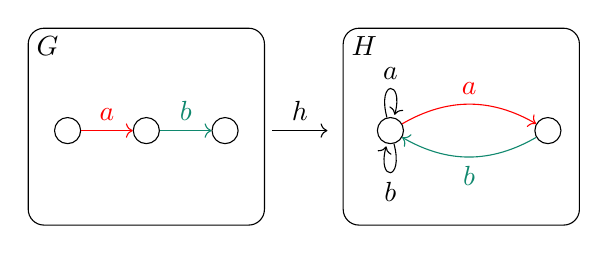
\begin{tikzpicture}
          \graphbox{$G$}{-40mm}{0mm}{30mm}{25mm}{0mm}{-3mm}{
            \coordinate (o) at (0mm,-10mm); 
            \node[draw,circle] (l1) at ($(o)+(-10mm,0mm)$) {};
            \node[draw,circle] (l2) at ($(l1)+(2,0)$) {};
            \node[draw,circle] (l3) at ($(l1)+(1,0)$) {};
            \draw[red,->] (l1) -- (l3) node[midway,above] {$a$};
            \draw[PineGreen,->] (l3) -- (l2) node[midway,above] {$b$};
        } 
            \graphbox{$H$}{0mm}{0mm}{30mm}{25mm}{-9mm}{-13mm}{
                \node[draw,circle] (1) at (0,0) {};
                \node[draw,circle] (2) at (2,0) {};
                \draw[->] (1) edge[loop above] node[midway, above] {$a$} (1);
                \draw[->] (1) edge[loop below] node[midway, below] {$b$} (1);
                \draw[->,red] (1) edge[bend left] node[midway, above] {$a$}  (2);
                \draw[->,PineGreen] (2) edge[bend left] node[midway, below] {$b$} (1);
            }
            % \node () at (-5mm,-15mm) {$\overset{h}{\to}$};
            \draw[->] (-9mm,-13mm) to node[midway,above] {$h$} (-2mm,-13mm);
        \end{tikzpicture}
          }
         \end{center}

    Colors show edge correspondence.
        \begin{center}
          \resizebox{0.7\textwidth}{!}{
        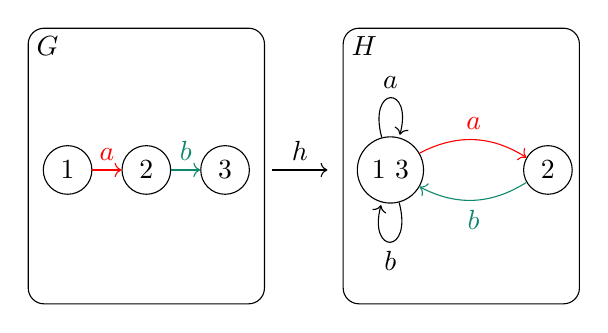
\begin{tikzpicture}
          \graphbox{$G$}{-40mm}{0mm}{30mm}{35mm}{0mm}{-8mm}{
            \coordinate (o) at (0mm,-10mm); 
            \node[draw,circle] (l1) at ($(o)+(-10mm,0mm)$) {1};
            \node[draw,circle] (l2) at ($(l1)+(2,0)$) {3};
            \node[draw,circle] (l3) at ($(l1)+(1,0)$) {2};
            \draw[red,->] (l1) -- (l3) node[midway,above] {$a$};
            \draw[PineGreen,->] (l3) -- (l2) node[midway,above] {$b$};
        } 
            \graphbox{$H$}{0mm}{0mm}{30mm}{35mm}{-9mm}{-18mm}{
                \node[draw,circle] (1) at (0,0) {1 3};
                \node[draw,circle] (2) at (2,0) {2};
                \draw[->] (1) edge[loop above] node[midway, above] {$a$} (1);
                \draw[->] (1) edge[loop below] node[midway, below] {$b$} (1);
                \draw[->,red] (1) edge[bend left] node[midway, above] {$a$}  (2);
                \draw[->,PineGreen] (2) edge[bend left] node[midway, below] {$b$} (1);
            }
            % \node () at (-5mm,-15mm) {$\overset{h}{\to}$};
            \draw[->] (-9mm,-18mm) to node[midway,above] {$h$} (-2mm,-18mm);
        \end{tikzpicture}
          }
         \end{center}

    Numbers show node correspondence.

    $h$ : morphism name
\end{frame}

\begin{frame}{Commutative Diagram}
    \begin{beamercolorbox}[rounded=true,shadow=true,wd=\textwidth]{block body}
        \begin{center}
            \resizebox{0.3\textwidth}{!}{
                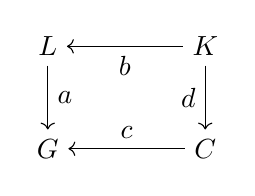
\begin{tikzpicture}
                    \node (I) at (0,-0.7) {$K$};
                    \node (L) at (-2,-0.7) {$L$};
                    \node (G) at (-2,-2) {$G$};
                    \node (C) at (0,-2) {$C$};
                    \draw [->] (I) to  node [midway,below] {$b$} (L);
                    \draw [->] (L) to node [midway,right] {$a$} (G);
                    \draw [->] (I) to node [midway,left] {$d$} (C);
                    \draw [->] (C) to node [midway,above] {$c$} (G);
                \end{tikzpicture}
            } 
        \end{center}
        commutes if \( a \circ b = c \circ d \).
    \end{beamercolorbox}
        
        \begin{center}
                \begin{tikzpicture}
                    \graphbox{}{0mm}{0mm}{34mm}{15mm}{2mm}{0mm}{
                        \coordinate (o) at (0mm,-8mm); 
                        \node[PineGreen,fill=PineGreen,circle] (l1) at ($(o)+(-10mm,0mm)$) {};
                        \node[red,fill=red,draw,circle] (l2) at ($(l1)+(2,0)$) {};
                        \node[draw,circle] (l3) at ($(l1)+(1,0)$) {};
                        \draw[->] (l1) -- (l3) node[midway,above] {};
                        \draw[->] (l3) -- (l2) node[midway,above] {};
                    } 
                    \graphbox{}{40mm}{0mm}{34mm}{15mm}{2mm}{0mm}{
                        \coordinate (o) at (0mm,-8mm); 
                        \node[PineGreen,fill=PineGreen,draw,circle] (l1) at ($(o)+(-10mm,0mm)$) {};
                        \node[red,fill=red,draw,circle] (l2) at ($(l1)+(2,0)$) {};
                    }  
                
                    \graphbox{ }{0mm}{-22mm}{34mm}{25mm}{2mm}{-5mm}{
                        \coordinate (o) at (0mm,-3mm); 
                        \node[PineGreen,fill=PineGreen,draw,circle] (l1) at ($(o)+(-10mm,0mm)$) {};
                        \node[red,fill=red,draw,circle] (l2) at ($(l1)+(2,0)$) {};
                        \node[draw,circle ] (l3) at ($(l1)+(1,0)$) {};
                        \node[blue,fill=blue,draw,circle] (l4) at ($(l2)+(0,-1)$) {};
                        \draw[->] (l1) -- (l3) node[midway,above] {};
                        \draw[->] (l3) -- (l2) node[midway,above] {};
                        \draw[->] (l2) -- (l4) node[midway,right] {};
                    }    
                    \graphbox{ }{40mm}{-22mm}{34mm}{25mm}{2mm}{-5mm}{
                        \coordinate (o) at (0mm,-3mm); 
                        \node[PineGreen,fill=PineGreen,draw,circle] (l1) at ($(o)+(-10mm,0mm)$) {};
                        \node[red,fill=red,draw,circle] (l2) at ($(l1)+(2,0)$) {};
                        \node[blue,fill=blue,draw,circle] (l4) at ($(l2)+(0,-1)$) {};
                        \draw[->] (l2) -- (l4) node[midway,right] {};
                    }    
                    \node () at (37mm,-8mm) {\( \underset{b}{\leftarrow} \)};  
                    \node () at (17mm,-18mm) {\( \downarrow\ a \)};
                    \node () at (37mm,-33mm) {\( \overset{c}{\leftarrow} \)};
                    \node () at (52mm,-18mm) {\( d\ \downarrow \)};
            \end{tikzpicture}
        \end{center}
\end{frame}

\begin{frame}{Pushouts: Gluing Graphs Along a common part}
\begin{beamercolorbox}[rounded=true,shadow=true,wd=\textwidth]{block body}
    The \textbf{pushout} of \((\alpha,\beta) \)
    is \begin{onlyenv}<2->
        \( \textcolor{red}{(\beta',\alpha')}\) with
    \end{onlyenv}
    \begin{itemize}
        % \item<2->{commutation:} \textcolor{red}{\( \beta' \mathop{\circ} \alpha  \mathop{=} \alpha'\mathop{\circ} \beta\)},
        \item<2-> $\square$\text{ABDC} commutative,
        % \item<3->{universality:}  \textcolor{PineGreen}{\( \forall \alpha \mathop{\star} \gamma' \mathop{=} \beta \mathop{\star} \gamma \Longrightarrow \exists~!~\delta. \gamma' \mathop{=} \beta' \mathop{\star} \delta  \gamma \mathop{=} \alpha' \mathop{\star} \delta \)}.
        \item<3->{universality:} \color{PineGreen}for all $(\gamma,\gamma')$,if $\square ABEC$ commutes, then there is a unique $\delta$ such that \text{$\triangle BDE$} and $\triangle CDE$ both commute.\color{black}
    \end{itemize} 
\end{beamercolorbox}
\hspace{-0.075\textwidth}% <-- exact horizontal gap between the two minipages
\begin{minipage}[t]{0.15\textwidth}
  \begin{overlayarea}{0.15\textwidth}{0.6\textheight}
    \begin{tikzpicture}[scale=0.8]
            \node (i) at (0,0) {A};
            \node (r) at (-1.5,-1) {B};
            \node (c) at (1.5,-1) {C};
            % \node () at (1,-1) {\( \Delta \)};
            \begin{onlyenv}<1->
                \draw[->]  (i) -- (r) node [pos=0.4,left] {$ \alpha $};
                \draw[->] (i) -- (c) node[pos=0.4, right] {$ \beta $};
            \end{onlyenv}
            \begin{onlyenv}<2->
                \node (h) at (0,-2) {\textcolor{red}{D}};
                    \draw[red,->] (c) -- (h) node [pos=0.8,right=1mm] {$ \alpha' $};
                \draw[red,->] (r) -- (h) node[pos=0.9, left=2mm] {$ \beta' $};
                \node () at (0,-1) {\textcolor{red}{PO}};
            \end{onlyenv}
            \begin{onlyenv}<3->
                \color{PineGreen}
                \node (d') at (0,-4) {E};
                \draw[->] (c) edge[bend left] node [midway,right]{$ \gamma $} (d') ;
                \draw[->] (r) edge[bend right] node [midway,left]{$ \gamma' $} (d') ;
                \draw[->,dashed] (h) -- (d') node [midway,right]{$ \delta $};
                \color{black}
            \end{onlyenv}
        \end{tikzpicture}
\end{overlayarea}
\end{minipage} 
\hspace{0.2\textwidth}% <-- exact horizontal gap between the two overlayareas
% Right box: width = 0.3\textwidth
\begin{minipage}[t]{0.25\textwidth}
  \begin{overlayarea}{0.25\textwidth}{0.6\textheight}
      \vspace{0.20\textheight}
        \begin{onlyenv}<4->
            \resizebox{6\textwidth}{!}{
                \rotatebox{-45}{
        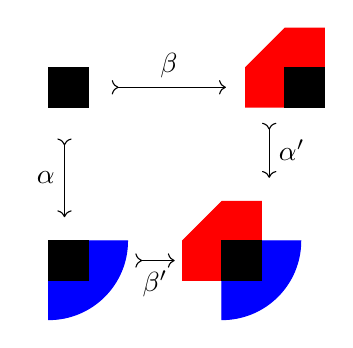
\begin{tikzpicture}  
            \coordinate (k) at (0, 0);
            \draw[black,fill=black] ($(k)+(0,0)$) rectangle ($(k)+(0.5,0.5)$);
            % \node () at ($(k)+(0.25,0.25)$) {\( \mathrm{K} \)};
        
            \coordinate (c) at (0, -2.2);
            \draw[fill=blue,blue]
            ($(c)+(0,-0.5)$)
            -- ($(c)+(0,0.5)$) 
            -- ($(c)+(1,0.5)$) 
            arc[start angle=0, end angle=-90, radius=1]
            -- cycle;
            % \node () at ($(c)+(0.75,0.25)$) {\( \mathrm{C'} \)};
            \draw[black,fill=black] ($(c)+(0,0)$) rectangle ($(c)+(0.5,0.5)$);
            % \node () at ($(c)+(0.25,0.25)$) {\( \mathrm{K} \)};
    
            \coordinate (r) at (3,0);
            \draw[fill=red,red] ($(r)+(-0.5,0)$)
            -- ($(r)+(-0.5,0.5)$)
            -- ($(r)+(0,1)$)
            --  ($(r)+(0.5,1)$)
            -- ($(r)+(0.5,0)$)
            -- cycle;
            % \node () at ($(r)+(-0.23,0.25)$) {\( \mathrm{R'} \)};
            \draw[black,fill=black] ($(r)+(0,0)$) rectangle ($(r)+(0.5,0.5)$);
            % \node () at ($(r)+(0.25,0.25)$) {\( \mathrm{K} \)};
        
            \coordinate (h) at (2.2, -2.2);
            \draw[fill=blue,blue]
            ($(h)+(0,-0.5)$)
            -- ($(h)+(0,0.5)$)
            -- ($(h)+(1,0.5)$) 
            arc[start angle=0, end angle=-90, radius=1]
            -- cycle;
            \draw[fill=red,red] ($(h)+(-0.5,0)$)
            -- ($(h)+(-0.5,0.5)$)
            -- ($(h)+(0,1)$)
            --  ($(h)+(0.5,1)$)
            -- ($(h)+(0.5,0)$)
            -- cycle;
        % \node () at ($(h)+(0.75,0.25)$) {\( \mathrm{C'} \)};
        \draw[black,fill=black] ($(h)+(0,0)$) rectangle ($(h)+(0.5,0.5)$);
        % \node () at ($(h)+(0.25,0.25)$) {\( \mathrm{K} \)};
        % \node () at ($(h)+(-0.23,0.25)$) {\( \mathrm{R'} \)};
        
            \draw[>->] ($(k)!0.5!(r)+(-0.7,0.25)$)
                    -- node[midway,above] {$\beta$}  
                ($(k)!0.5!(r)+(0.75,0.25)$);
            % \node (kr) at ($(k)!0.5!(r)+(0.25,0.25)$)
            % {\( \overset{\rightarrowtail}{s} \)};
            % ;  
            \draw[>->]($(c)!0.5!(h)+(0,0.25)$)
                    -- node[midway,below]  {$\beta'$}  
                ($(c)!0.5!(h)+(0.5,0.25)$);
              
                \draw[<-<]($(k)!0.5!(c)+(0.2,-0.3)$)
                    -- node[midway,left]  {$\alpha$}  
                ($(k)!0.5!(c)+(0.2,0.7)$);
               
                \draw[>->]($(r)!0.5!(h)+(0.2,0.9)$)
                    -- node[midway,right]  {$\alpha'$}  
                ($(r)!0.5!(h)+(0.2,0.2)$);
        \end{tikzpicture}
                }
        }
    \end{onlyenv}
    \end{overlayarea}
\end{minipage}
\hspace{0.25\textwidth}% small gap
\begin{minipage}[t]{0.38\textwidth}
  \begin{overlayarea}{0.4\textwidth}{0.6\textheight}
    \begin{onlyenv}<5->
        \resizebox{!}{1.4\textwidth}{
                \rotatebox{-45}{
             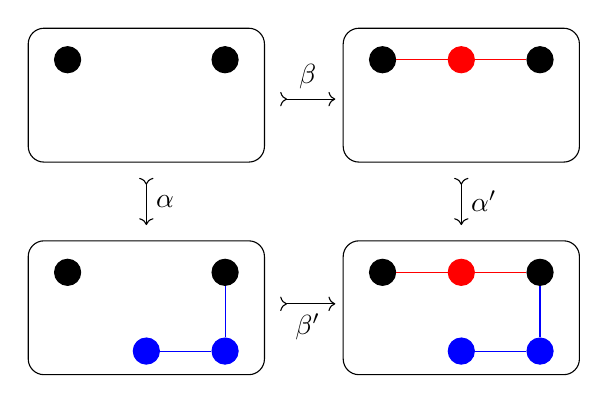
\begin{tikzpicture}
              \graphbox{}{0mm}{5mm}{30mm}{17mm}{2mm}{-5mm}{
                 \coordinate (o) at (-2mm,1mm); 
                  \node[black,fill=black,draw,circle] (l1) at ($(o)+(-10mm,0mm)$) {};
                  \node[black,fill=black,draw,circle] (l2) at ($(l1)+(2,0)$) {};
              } 

              \graphbox{}{40mm}{5mm}{30mm}{17mm}{2mm}{-5mm}{
                \coordinate (o) at (-2mm,1mm); 
                  \node[black,fill=black,draw,circle] (l1) at ($(o)+(-10mm,0mm)$) {};
                  \node[black,fill=black,draw,circle] (l2) at ($(l1)+(2,0)$) {};
                  \node[red,draw,circle,fill=red] (l3) at ($(l1)+(1,0)$) {};
                  \draw[red] (l1) -- (l3) node[midway,above] {};
                  \draw[red] (l3) -- (l2) node[midway,above] {};
              }  

              \graphbox{}{0mm}{-22mm}{30mm}{17mm}{2mm}{-5mm}{
                \coordinate (o) at (-2mm,1mm);
                  \node[black,fill=black,draw,circle] (l1) at ($(o)+(-10mm,0mm)$) {};
                  \node[black,fill=black,draw,circle] (l2) at ($(l1)+(2,0)$) {};
                  \node[blue,draw,circle,fill=blue] (l4) at ($(l2)+(0,-1)$) {};
                  \draw[blue] (l2) -- (l4) node[midway,right] {};
                %   \node[blue,draw,circle] (l6) at ($(l1)+(0,-1)$) {7};
                %   \draw[blue,<-] (l1) -- (l6) node[midway,left] {$a$};
                    \node[blue,draw,circle,fill=blue] (l7) at ($(l4)+(-1,0)$) {};
                  \draw[blue] (l4) -- (l7) node[midway,below] {};
              }    

              \graphbox{}{40mm}{-22mm}{30mm}{17mm}{2mm}{-5mm}{
                \coordinate (o) at (-2mm,1mm);
                  \node[black,fill=black,draw,circle] (l1) at ($(o)+(-10mm,0mm)$) {};
                  \node[black,fill=black,draw,circle] (l2) at ($(l1)+(2,0)$) {};
                  \node[red,draw,circle,fill=red] (l3) at ($(l1)+(1,0)$) {};
                  \node[blue,draw,circle,fill=blue] (l4) at ($(l2)+(0,-1)$) {};
                  \draw[red] (l1) -- (l3) node[midway,above] {};
                  \draw[red] (l3) -- (l2) node[midway,above] {};
                  \draw[blue] (l2) -- (l4) node[midway,right] {};
                %   \node[blue,draw,circle] (l6) at ($(l1)+(0,-1)$) {7};
                %   \draw[blue,<-] (l1) -- (l6) node[midway,left] {$a$};
                \node[blue,draw,circle,fill=blue] (l7) at ($(l4)+(-1,0)$) {};
                  \draw[blue] (l4) -- (l7) node[midway,below] {};
              }    

              % \node () at (37mm,-8mm) {\( \underset{\rightarrowtail}{\beta} \)}; % K -> L
              \draw[>->] (32mm,-4mm) to node[midway,above] {$\beta$} (39mm,-4mm);
              % \node () at (17mm,-18mm) {\(\alpha\ \downarrowtail  \)};
              \draw[>->] (15mm,-14mm) to node[midway,right] {$\alpha$} (15mm,-20mm);
              % \node () at (37mm,-33mm) {\( \overset{\rightarrowtail}{\beta'} \)};
              \draw[>->] (32mm,-30mm) to node[midway,below] {$\beta'$} (39mm,-30mm);
              % \node () at (52mm,-18mm) {\( \downarrowtail\ \alpha' \)};
              \draw[>->] (55mm,-14mm) to node[midway,right] {$\alpha'$} (55mm,-20mm);
      \end{tikzpicture}
                }
        }
    \end{onlyenv}
  \end{overlayarea}
\end{minipage}
\end{frame}
 

\subsection{Graph Rewriting with Double-Pushout (DPO)}
\begin{frame}{Graph Rewriting with Double-Pushout (DPO)}
    \begin{overlayarea}{\textwidth}{\textheight}
    \begin{beamercolorbox}[rounded=true,shadow=true,wd=\textwidth]{block body}
        \resizebox{!}{0.25\textheight}{
            \begin{tikzpicture}
                \begin{onlyenv}<1->
                    \node (I) at (0,0) {$K$};
                    \node (L) at (-2,0) {$L$};
                    \node (R) at (2,0) {$R$};
                    \draw [->] (I) to  node [midway,above] {$l$} (L);
                    \draw [->] (I) to  node [midway,above] {$r$} (R);
                    \draw[fill=red,opacity=0.1 , rounded corners, dotted] (-2.5,-0.5) rectangle (2.5,0.5);
                    \node () at (5.5,0) {Rewriting rule with \textcolor{red}{interface $K$}};
                \end{onlyenv} 
                \begin{onlyenv}<2->
                    \node (G) at (-2,-1.5) {$G$};
                    \draw [>->] (L) to node [midway,right] {} (G);
                \end{onlyenv}
                \begin{onlyenv}<3->
                    \node (C) at (0,-1.5) {$C$};
                    \draw [->] (I) to node [midway,right] { } (C);
                    \node [at=($(I)!.5!(G)$)] {\normalfont PO};
                    \draw [->] (C) to node [midway,above] { } (G);
                \end{onlyenv}
                \begin{onlyenv}<4->
                    \node (H) at (2,-1.5) {$H$};
                    \draw [->] (R) to node [midway,left] { } (H);
                    \draw [->] (C) to node [midway,above] { } (H);
                    \node [at=($(I)!.5!(H)$)] {\normalfont PO};
                    \draw[fill=PineGreen,opacity=0.1 , rounded corners, dotted] (-2.5,-2) rectangle (2.5,-1);
                    \node () at (5.5,-1.5) {\text{rewriting step $G \Rightarrow H$}};
                \end{onlyenv}
                \end{tikzpicture}
        }
    \end{beamercolorbox}
    \vspace{-0.07\textheight}
  \begin{center}
    \resizebox{\textwidth}{!}{
      \begin{tikzpicture}
            \begin{onlyenv}<1->
                 \graphbox{\( L \)}{0mm}{5mm}{34mm}{15mm}{2mm}{0mm}{
                  \coordinate (o) at (0mm,-8mm); 
                  \node[draw,circle] (l1) at ($(o)+(-10mm,0mm)$) {1};
                  \node[draw,circle] (l2) at ($(l1)+(2,0)$) {2};
                  \node[orange,draw,circle] (l3) at ($(l1)+(1,0)$) {3};
                  \draw[orange,->] (l1) -- (l3) node[midway,above] {$a$};
                  \draw[orange,->] (l3) -- (l2) node[midway,above] {$a$};
              } 

              \graphbox{\( K \)}{40mm}{5mm}{34mm}{15mm}{2mm}{0mm}{
                  \coordinate (o) at (0mm,-8mm); 
                  \node[draw,circle] (l1) at ($(o)+(-10mm,0mm)$) {1};
                  \node[draw,circle] (l2) at ($(l1)+(2,0)$) {2};
              }  

              \graphbox{\( R\)}{80mm}{5mm}{45mm}{15mm}{2mm}{0mm}{
                  \coordinate (o) at (-5mm,-8mm); 
                  \node[draw,circle] (l1) at ($(o)+(-10mm,0mm)$) {1};
                  \node[draw,circle] (l2) at ($(l1)+(3,0)$) {2};
                  \node[red,draw,circle] (l3) at ($(l1)+(1,0)$) {4};
                  \node[red,draw,circle] (l4) at ($(l1)+(2,0)$) {5};
                  \draw[red,->] (l1) -- (l3) node[midway,above] {$a$};
                  \draw[red,->] (l3) -- (l4) node[midway,above] {$b$};
                  \draw[red,->] (l4) -- (l2) node[midway,above] {$a$};
              }    
              \node () at (37mm,-3mm) {\( \overset{l}{\leftarrow} \)}; 
              \node () at (77mm,-3mm) {\( \overset{r}{\rightarrow} \)}; 
            \end{onlyenv} 
            \begin{onlyenv}<2->
                \graphbox{\( G  \)}{0mm}{-17mm}{34mm}{25mm}{2mm}{-5mm}{
                  \coordinate (o) at (0mm,-3mm); 
                  \node[draw,circle] (l1) at ($(o)+(-10mm,0mm)$) {1};
                  \node[draw,circle] (l2) at ($(l1)+(2,0)$) {2};
                  \node[draw,circle,orange] (l3) at ($(l1)+(1,0)$) {3};
                  \node[blue, draw,circle] (l4) at ($(l2)+(0,-1)$) {6};
                  \draw[orange,->] (l1) -- (l3) node[midway,above] {$a$};
                  \draw[orange,->] (l3) -- (l2) node[midway,above] {$a$};
                  \draw[blue,->] (l2) -- (l4) node[midway,right] {$a$};
              }   
              \node () at (17mm,-13mm) {\( \downarrowtail \)};
            \end{onlyenv}
            \begin{onlyenv}<3-> 
                \graphbox{\( C  \)}{40mm}{-17mm}{34mm}{25mm}{2mm}{-5mm}{
                  \coordinate (o) at (0mm,-3mm); 
                  \node[draw,circle] (l1) at ($(o)+(-10mm,0mm)$) {1};
                  \node[draw,circle] (l2) at ($(l1)+(2,0)$) {2};
                  \node[blue,draw,circle] (l4) at ($(l2)+(0,-1)$) {6};
                  \draw[blue,->] (l2) -- (l4) node[midway,right] {$a$};
                 }   
                \node () at (37mm,-28mm) {\( \leftarrow \)};
                 \node () at (52mm,-13mm) {\( \downarrow \)};
                 \node () at (37mm,-15mm) {\text{PO}};
            \end{onlyenv}
            \begin{onlyenv}<4-> 
              \graphbox{\( H   \)}{80mm}{-17mm}{45mm}{25mm}{2mm}{-5mm}{
                  \coordinate (o) at (-5mm,-3mm); 
                  \node[draw,circle] (l1) at ($(o)+(-10mm,0mm)$) {1};
                  \node[draw,circle] (l2) at ($(l1)+(3,0)$) {2};
                  \node[draw,circle,red] (l3) at ($(l1)+(1,0)$) {4};
                  \node[draw,circle,red] (l4) at ($(l1)+(2,0)$) {5};
                  \node[blue,draw,circle] (l5) at ($(l2)+(0,-1)$) {6};
                  \draw[red,->] (l1) -- (l3) node[midway,above] {$a$};
                  \draw[red,->] (l3) -- (l4) node[midway,above] {$b$};
                  \draw[red,->] (l4) -- (l2) node[midway,above] {$a$};
                  \draw[blue,->] (l2) -- (l5) node[midway,right] {$a$};
              }    
              \node () at (92mm,-13mm) {\( \downarrow \)};
              \node () at (77mm,-28mm) {\( \rightarrow \)}; 
                 \node () at (77mm,-15mm) {\text{PO}};
            \end{onlyenv} 
            
      \end{tikzpicture}
      }
   \end{center}
\end{overlayarea}
\end{frame}

\begin{frame}{An Invalid Rewriting Step}
    % of the edge \textcolor{red}{$3 \overset{a}{\rightarrow} 6$} in $G$:
    \begin{center}
        \resizebox{\textwidth}{!}{
        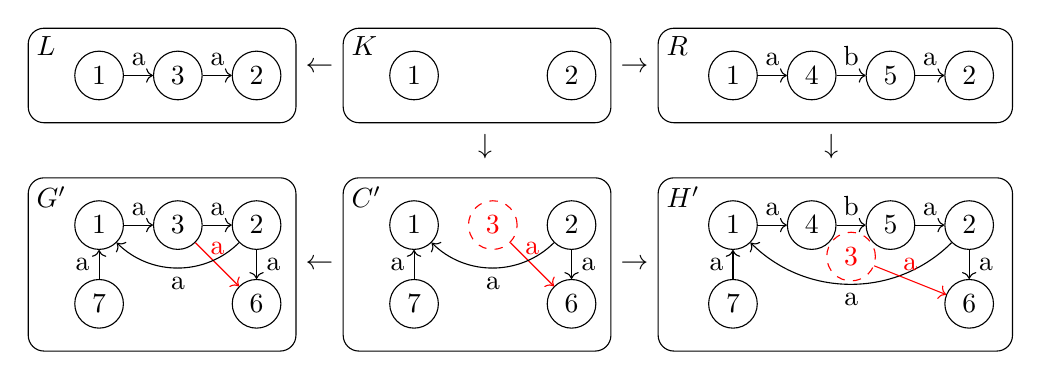
\begin{tikzpicture}
            \graphbox{\( L \)}{0mm}{-3mm}{34mm}{12mm}{2mm}{2mm}{
                \coordinate (o) at (0mm,-8mm); 
                \node[draw,circle] (l1) at ($(o)+(-10mm,0mm)$) {1};
                \node[draw,circle] (l2) at ($(l1)+(2,0)$) {2};
                \node[draw,circle] (l3) at ($(l1) + (1,0)$) {3};
                \draw[->] (l1) -- (l3) node[midway,above] {a};
                \draw[->] (l3) -- (l2) node[midway,above] {a};
            } 
    
            \graphbox{\( K \)}{40mm}{-3mm}{34mm}{12mm}{2mm}{2mm}{
                \coordinate (o) at (0mm,-8mm); 
                \node[draw,circle] (l1) at ($(o)+(-10mm,0mm)$) {1};
                \node[draw,circle] (l2) at ($(l1)+(2,0)$) {2};
            }  
    
            \graphbox{\( R \)}{80mm}{-3mm}{45mm}{12mm}{2mm}{2mm}{
                \coordinate (o) at (-5mm,-8mm); 
                \node[draw,circle] (l1) at ($(o)+(-10mm,0mm)$) {1};
                \node[draw,circle] (l2) at ($(l1)+(3,0)$) {2};
                \node[draw,circle] (l3) at ($(l1) + (1,0)$) {4};
                \node[draw,circle] (l4) at ($(l1) + (2,0)$) {5};
                \draw[->] (l1) -- (l3) node[midway,above] {a};
                \draw[->] (l3) -- (l4) node[midway,above] {b};
                \draw[->] (l4) -- (l2) node[midway,above] {a};
            }    
    
            \graphbox{\( G' \)}{0mm}{-22mm}{34mm}{22mm}{2mm}{-3mm}{
                \coordinate (o) at (0mm,-3mm); 
                \node[draw,circle] (l1) at ($(o)+(-10mm,0mm)$) {1};
                \node[draw,circle] (l2) at ($(l1)+(2,0)$) {2};
                \node[draw,circle] (l3) at ($(l1) + (1,0)$) {3};
                \node[draw,circle] (l4) at ($(l2) + (0,-1)$) {6};
                \draw[->,red] (l3) -- (l4) node[midway,above] {a};
                \draw[->] (l1) -- (l3) node[midway,above] {a};
                \draw[->] (l3) -- (l2) node[midway,above] {a};
                \draw[->] (l2) -- (l4) node[midway,right] {a};
                \node[draw,circle] (l6) at ($(l1) + (0,-1)$) {7};
                \draw[<-] (l1) -- (l6) node[midway,left] {a};
                \draw[->] (l2) edge[out=-135,in=-45]node[midway,below] {a} (l1) ;
            }    
    
            \graphbox{\( C'  \)}{40mm}{-22mm}{34mm}{22mm}{2mm}{-3mm}{
                \coordinate (o) at (0mm,-3mm); 
                \node[draw,circle] (l1) at ($(o)+(-10mm,0mm)$) {1};
                \node[draw,circle] (l2) at ($(l1)+(2,0)$) {2};
                \node[draw,circle] (l4) at ($(l2) + (0,-1)$) {6};
                \node[draw,circle,dashed,red] (l3) at ($(l1) + (1,0)$) {3};
                % \draw[->,red] (l3) -- (l4) node[midway,above] {a};
                \draw[->,red] (l3) -- (l4) node[midway,above] {a};
                \draw[->] (l2) -- (l4) node[midway,right] {a};
                \draw[->] (l2) edge[out=-135,in=-45]node[midway,below] {a} (l1) ;
                \node[draw,circle] (l6) at ($(l1) + (0,-1)$) {7};
                \draw[<-] (l1) -- (l6) node[midway,left] {a};
            }    
    
            \graphbox{\( H' \)}{80mm}{-22mm}{45mm}{22mm}{2mm}{-3mm}{
                \coordinate (o) at (-5mm,-3mm); 
                \node[draw,circle] (l1) at ($(o)+(-10mm,0mm)$) {1};
                \node[draw,circle] (l2) at ($(l1)+(3,0)$) {2};
                \node[draw,circle] (l3) at ($(l1) + (1,0)$) {4};
                \node[draw,circle] (l4) at ($(l1) + (2,0)$) {5};
                \node[draw,circle] (l5) at ($(l2) + (0,-1)$) {6};
                \node[draw,circle] (l6) at ($(l1) + (0,-1)$) {7};
                \draw[<-] (l1) -- (l6) node[midway,left] {a};
                \draw[->] (l1) -- (l3) node[midway,above] {a};
                \draw[->] (l3) -- (l4) node[midway,above] {b};
                \draw[->] (l4) -- (l2) node[midway,above] {a};
                \draw[->] (l2) -- (l5) node[midway,right] {a};
                \draw[->] (l2) edge[out=-135,in=-45]node[midway,below] {a} (l1) ;
                \node[draw,circle,dashed,red] (l3) at (-0mm,-7mm) {3};
                \draw[->,red] (l3) -- (l5) node[midway,above] {a};
            }    
    
            \node () at (37mm,-8mm) {\( \leftarrow \)}; % K -> L
            \node () at (77mm,-8mm) {\( \rightarrow \)}; % K -> R
            \node () at (15mm,-18mm) {\(\downarrowtail \)};
            \node () at (37mm,-33mm) {\( \leftarrow \)};
            % \node () at (37mm,-18mm) {PO};
            \node () at (58mm,-18mm) {\( \downarrow \)}; 
            % \node () at (80mm,-18mm) {PO};
            \node () at (102mm,-18mm) {\( \downarrow \)};
            \node () at (77mm,-33mm) {\( \rightarrow \)}; % C -> H
        \end{tikzpicture}
        }         
    \end{center}
    No implicit edge deletion by construction
\end{frame}

\section{Toward greater usability}
\begin{frame}
  \tableofcontents[currentsection, hideothersubsections]
\end{frame}

\begin{frame}{Weighted Type Graph Method~\cite{bruggink2014termination,bruggink2015proving,endrullis2024generalized_icgt}}
Termination by interpretation
\newline\newline
Parameter: an object $T$ in the category, called \textcolor{PineGreen}{type graph}
\newline\newline
Terminology: every graph is \enquote{typed} as morphisms to $T$
\newline\newline
Interpretation:
\vspace{-3mm}
\begin{flalign*}
G &\leadsto \mathcal{F}(G,T) \\
  &\leadsto \mathrm{weight}(\mathcal{F}(G,T)) \\
  &\leadsto \mathrm{aggregator}(\mathrm{weight}(\mathcal{F}(G,T)))\in\mathbb{N}
\end{flalign*}

% \only<2->{
\alert{
What is the morphism weight?
\newline\newline
What is the graph weight?}
% }
\end{frame}


\begin{frame}{Weighted Type Graph}
    \begin{overlayarea}{\textwidth}{\textheight}
        \begin{beamercolorbox}[rounded=true,shadow=true,wd=\textwidth]{block body}
           A weighted type graph is a graph with weights on edges.
        \end{beamercolorbox}
 
        \begin{center}
        \begin{tikzpicture}
            \graphbox{T}{0mm}{0mm}{32mm}{28mm}{-10mm}{-14mm}{
                \node[draw,circle] (1) at (0,0) {};
                \node[draw,circle] (2) at (2,0) {};
                    % \begin{onlyenv}<1>
                    %     \draw[->] (1) edge[loop above] node[midway, above] {$a$} (1);
                    %     \draw[->] (1) edge[loop below] node[midway, below] {$b$} (1) ;
                    %     \draw[->] (1) edge[bend left] node[midway, above] {$a$}  (2)  ;
                    %     \draw[->] (2) edge[bend left] node[midway, below] {$a$} (1)   ;
                    % \end{onlyenv}
                    \begin{onlyenv}<1->
                        \draw[->] (1) edge[loop above] node[midway, above] {$a^{\textcolor{red}{1}}$} (1);
                        \draw[->] (1) edge[loop below] node[midway, below] {$b^{\textcolor{red}{0}}$} (1) ;
                        \draw[->] (1) edge[bend left] node[midway, above] {$a^{\textcolor{red}{0}}$}  (2)  ;
                        \draw[->] (2) edge[bend left] node[midway, below] {$b^{\textcolor{red}{0}}$} (1)   ;
                    \end{onlyenv}
                    
            }
        \end{tikzpicture}
        \end{center}
        
    \end{overlayarea}

\end{frame}

\begin{frame}{Morphism Weight}
    \begin{beamercolorbox}[rounded=true,shadow=true,wd=\textwidth]{block body}
      The weight of a morphism $h: G \rightarrow T$ is \[\sum_{e \in \opn{Edge(G)}}\mathrm{weight}(h(e)) \]
    \end{beamercolorbox}
    \begin{center}
    \resizebox{0.8\textwidth}{!}{
        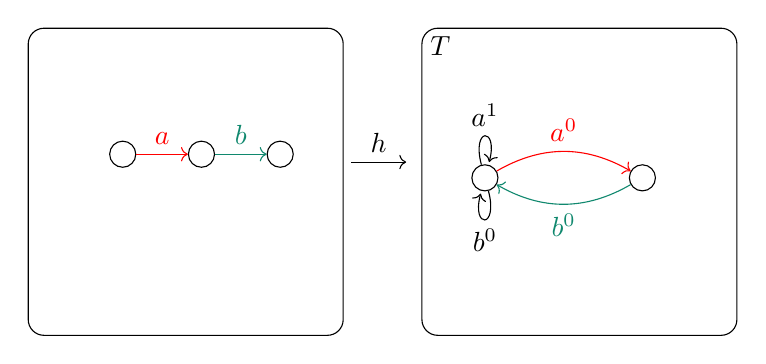
\begin{tikzpicture}
          \graphbox{}{-50mm}{0mm}{40mm}{39mm}{2mm}{-6mm}{
            \coordinate (o) at (0mm,-10mm); 
            \node[draw,circle] (l1) at ($(o)+(-10mm,0mm)$) {};
            \node[draw,circle] (l2) at ($(l1)+(2,0)$) {};
            \node[draw,circle] (l3) at ($(l1)+(1,0)$) {};
            \draw[red,->] (l1) -- (l3) node[midway,above] {$a$};
            \draw[PineGreen,->] (l3) -- (l2) node[midway,above] {$b$};
        } 
            \graphbox{$T$}{0mm}{0mm}{40mm}{39mm}{-12mm}{-19mm}{
                \node[draw,circle] (1) at (0,0) {};
                \node[draw,circle] (2) at (2,0) {};
                \draw[->] (1) edge[loop above] node[midway, above] {$a^{1}$} (1);
                \draw[->] (1) edge[loop below] node[midway, below] {$b^{0}$} (1);
                \draw[->,red] (1) edge[bend left] node[midway, above] {$a^{0}$}  (2);
                \draw[->,PineGreen] (2) edge[bend left] node[midway, below] {$b^{0}$} (1);
            }
            % \node () at (-5mm,-15mm) {$\overset{h}{\to}$};
            \draw[->] (-9mm,-17mm) to node[midway,above] {$h$} (-2mm,-17mm);
        \end{tikzpicture}
        }
    \end{center}

        $ \opn{weight}_T(h) \mathop{=} \textcolor{red}{0} + \textcolor{PineGreen}{0} \mathop{=} 0$

\end{frame}
 

\begin{frame}{Graph Weight} 
    \begin{beamercolorbox}[rounded=true,shadow=true,wd=\textwidth]{block body}
        The weight of a graph $L$ is \[\min \{h : L \mathop{\to} T \mid \mathrm{weight}_T(h)\}\]
    \end{beamercolorbox}
    \begin{center}
        \resizebox{1\textwidth}{!}{
            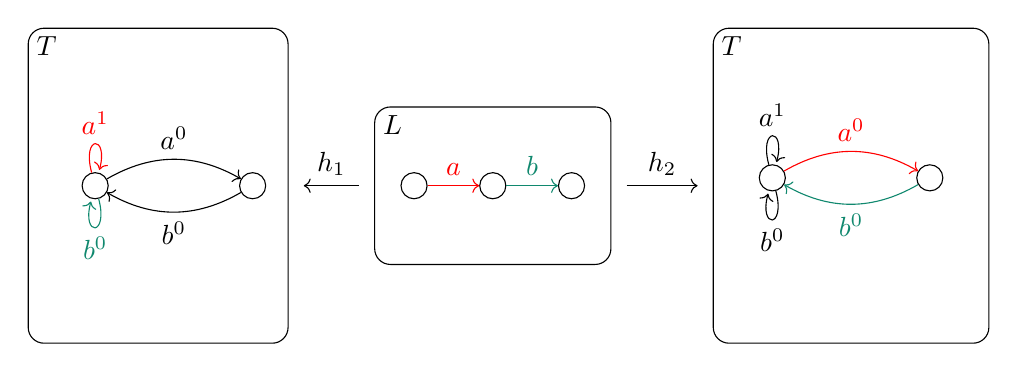
\begin{tikzpicture}
                \graphbox{\(L\)}{2mm}{0mm}{30mm}{20mm}{0mm}{0mm}{
                    \coordinate (o) at (0mm,-10mm); 
                    \node[draw,circle] (l1) at ($(o)+(-10mm,0mm)$) {};
                    \node[draw,circle] (l2) at ($(l1)+(2,0)$) {};
                    \node[draw,circle] (l3) at ($(l1)+(1,0)$) {};
                    \draw[->,red] (l1) -- (l3) node[midway,above] {$a$};
                    \draw[->,PineGreen] (l3) -- (l2) node[midway,above] {$b$};
                } 
                \graphbox{$T$}{-42mm}{10mm}{33mm}{40mm}{-8mm}{-20mm}{
                    \node[draw,circle] (1) at (0,0) {};
                    \node[draw,circle] (2) at (2,0) {};
                    \draw[->,red] (1) edge[loop above] node[midway, above] {$a^{1}$} (1) ;
                    \draw[->,PineGreen] (1) edge[loop below] node[midway, below] {$b^{0}$} (1) ;
                    \draw[->] (1) edge[bend left] node[midway, above] {$a^{0}$}  (2)  ;
                    \draw[->] (2) edge[bend left] node[midway, below] {$b^{0}$} (1) ;
                }
            
                \graphbox{$T$}{45mm}{10mm}{35mm}{40mm}{-10mm}{-19mm}{
                    \node[draw,circle] (1) at (0,0) {};
                    \node[draw,circle] (2) at (2,0) {};
                    \draw[->] (1) edge[loop above] node[midway, above] {$a^{1}$} (1) ;
                    \draw[->] (1) edge[loop below] node[midway, below] {$b^{0}$} (1) ;
                    \draw[->,red] (1) edge[bend left] node[midway, above] {$a^{0}$}  (2)  ;
                    \draw[->,PineGreen] (2) edge[bend left] node[midway, below] {$b^{0}$} (1);
                }
                % \node () at (43mm,-10mm) {$\overset{h_2}{\to}$};
                \draw[->] (34mm,-10mm) to node[midway,above] {$h_2$} (43mm,-10mm);
                % \node () at (-3mm,-10mm) {$\overset{h_1}{\leftarrow}$};
                \draw[<-] (-7mm,-10mm) to node[midway,above] {$h_1$} (0mm,-10mm);
            \end{tikzpicture}
            }
    \end{center}
    \begin{flalign*}
      & \mathrm{weight}_T(h_1) = \textcolor{red}{1} + \textcolor{PineGreen}{0} = \textcolor{red}{1} \hspace{0.1\textwidth} &\mathrm{weight}_T(h_2) = \textcolor{red}{0} + \textcolor{PineGreen}{0} = \textcolor{PineGreen}{0}\\
      &\mathrm{weight}_T(L) = \min \{\textcolor{red}{1}, \textcolor{PineGreen}{0}\} = 0 &
    \end{flalign*}
        % $\mathrm{weight}_T(L) \mathop{=} \min \{,\mathrm{weight}_T(h_2)\} = \min \{1+1, 1+0\}\mathop{=} 1$       
\end{frame}

% \begin{frame}
%     \begin{center}
%         \resizebox{0.3\textwidth}{!}{
%             \begin{tikzpicture}
%             \graphbox{$R$}{0mm}{0mm}{45mm}{15mm}{2mm}{-10mm}{
%                 \coordinate (o) at (-5mm,0mm); 
%                 \node[draw,circle] (l1) at ($(o)+(-10mm,0mm)$) {1};
%                 \node[draw,circle] (l2) at ($(l1)+(3,0)$) {2};
%                 \node[draw,circle] (l3) at ($(l1)+(1,0)$) {4};
%                 \node[draw,circle] (l4) at ($(l1)+(2,0)$) {5};
%                 \draw[->] (l1) -- (l3) node[midway,above] {$a$};
%                 \draw[->] (l3) -- (l4) node[midway,above] {$b$};
%                 \draw[->] (l4) -- (l2) node[midway,above] {$a$};
%             } 
%             \end{tikzpicture}
%         }
%     \end{center}
%     has three morphisms to $T$:
%         \newline
%         \begin{center}
%             \resizebox{0.3\textwidth}{!}{
%                 \begin{tikzpicture}
%                     \graphbox{$T$}{0mm}{0mm}{45mm}{50mm}{-10mm}{-25mm}{
%                         \node[draw,circle] (1) at (0,0) {$1\ 2\ 4\ 5$};
%                         \node[draw,circle] (2) at (2,0) {};
%                         \draw[->,red] (1) edge[loop above] node[midway, above] {$a^{1}$} (1) ;
%                         \draw[->,red] (1) edge[loop below] node[midway, below] {$b^{0}$} (1);
%                         \draw[->] (1) edge[bend left] node[midway, above] {$a^{0}$}  (2);
%                         \draw[->] (2) edge[bend left] node[midway, below] {$b^{0}$} (1);
%                     }
%                 \end{tikzpicture}
%                 }
%             \resizebox{0.3\textwidth}{!}{
%             \begin{tikzpicture}
%                 \graphbox{$T$}{0mm}{0mm}{45mm}{50mm}{-10mm}{-25mm}{
%                     \node[draw,circle] (1) at (0,0) {$1\ 2\ 5$};
%                     \node[draw,circle] (2) at (2,0) {$4$};
%                     \draw[->,red] (1) edge[loop above] node[midway, above] {$a^{1}$} (1) ;
%                     \draw[->] (1) edge[loop below] node[midway, below] {$b^{0}$} (1) ;
%                     \draw[->,red] (1) edge[bend left] node[midway, above] {$a^{0}$}  (2)  ;
%                     \draw[->,red] (2) edge[bend left] node[midway, below] {$b^{0}$} (1);
%                 }
%             \end{tikzpicture}
%             }
%             \resizebox{0.3\textwidth}{!}{
%                 \begin{tikzpicture}
%                     \graphbox{$T$}{0mm}{0mm}{45mm}{50mm}{-10mm}{-25mm}{
%                         \node[draw,circle ] (1) at (0,0) {$1\ 5$};
%                         \node[draw,circle] (2) at (2,0) {$4\ 2$};
%                         \draw[->] (1) edge[loop above] node[midway, above] {$a^{1}$} (1) ;
%                         \draw[->] (1) edge[loop below] node[midway, below] {$b^{0}$} (1) ;
%                         \draw[->,red] (1) edge[bend left] node[midway, above] {$a^{0}$}  (2)  ;
%                         \draw[->,red] (2) edge[bend left] node[midway, below] {$b^{0}$} (1);
%                     }
%                 \end{tikzpicture}
%             }
%     \end{center}

      
%      $\opn{weight}_T(R) = \min \{1+0+1, 0+0+1, 0 + 0 + 0\}\mathop{=} 0$.
% \end{frame}
   
\begin{frame}{Termination Criterion~\cite{bruggink2015proving}}
    %   \begin{beamercolorbox}[rounded=true,shadow=true,wd=\textwidth]{block body}
    \begin{center}
    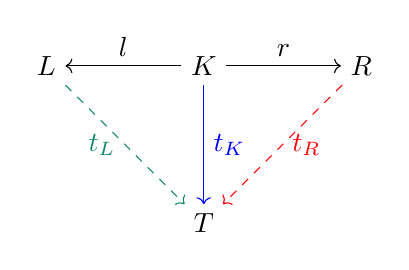
\begin{tikzpicture}
            \node (k) at (0,0) {$K$};
            \node (l) at (-2,0) {$L$};
            \node (t) at (0,-2) {$T$};
            \node (r) at (2,0) {$R$};
            \draw [->] (k) to  node [midway,above] {$l$} (l);
            \draw [->] (k) to  node [midway,above] {$r$} (r);
            \draw [->,blue] (k) to  node [midway,right] {\textcolor{blue}{$t_K$}} (t);
            \draw [->,dashed,PineGreen] (l) to node [midway,left] {\textcolor{PineGreen}{$t_L$}} (t);
            \draw [->,dashed,red] (r) to node [midway,right] {\textcolor{red}{$t_R$}} (t);
        \end{tikzpicture}
    \end{center}

      \begin{beamercolorbox}[rounded=true,shadow=true,wd=\textwidth]{block body}
        Every rewriting step strictly decreases the weight if 
        \begin{itemize}
        \item for all \textcolor{blue}{$t_K$}, if there is \textcolor{PineGreen}{$t_L$} such that $\triangle KLT$ commutes, then 
        \begin{flalign*}
            &\min \{\opn{weight}_T(\textcolor{PineGreen}{t_L}) \mid t_L.\triangle KLT \text{commutes}\}  
            \\ \mathop{>}
            &\min \{\opn{weight}_T(\textcolor{red}{t_R}) \mid t_R.\triangle KRT \text{commutes}\}  
        \end{flalign*}
        \end{itemize} 
    \end{beamercolorbox}
 
   \alert{How to find a suitable weighted type graph?}
\end{frame}
\begin{frame}{Searching for Weighted Type Graphs over $\mathbb{N}$}
    User-specified parameters:
      \begin{itemize}
        \item \alert{$k$ nodes}
        \item \alert{maximum edge weight $n\in\mathbb{N}$}
      \end{itemize}   
    Assumption:
      \begin{itemize}
        \item no parallel edges of the same label 
      \end{itemize}
    The problem amounts to checking the \textcolor{red}{satisfiability of an
existential Presburger arithmetic theory} with:
                \begin{itemize}
                  \item $k^2m$ binary variables where $m$ is the number of labels
                  \item $k^2m$ integer variables
                \end{itemize} 
  Challenge:
  \begin{itemize}
    \item $2^{k^2m} \cdot n^{k^2m}$ possible assignments of weights
    \item maximum edge weight hard to guess
  \end{itemize} 
\end{frame}


\begin{frame}{Problem of the Size of the Search Space}
% def f(k, m, n) -> int:
%     e = pow(k,2) * m
%     left = pow(2,e)
%     right = pow(n,e)
%     return left * right
With natural numbers as weights:
    \begin{center}
    \begin{tabular}{ |c|c|c|c| } 
    \hline
    \# nodes (k)&  \# labels (m) & \# weights & \# possibilities \\ 
    \hline
    2 & 2 & 2 & $\approx 10^{4}$ \\ 
    \hline
    3 & 3 & 3 & $\approx  10^{21}$ \\ 
    \hline
    3 & 3 & 10 & $\approx   10^{45}$ \\
    \hline
    3 & 3 & 100 & $\approx 10^{87}$ \\
    \hline
    4 & 4 & 4 & $\approx  10^{57}$ \\ 
    \hline
    4 & 4 & 10 & $\approx 10^{95}$ \\
     \hline
    4 & 4 & 100 & $\approx 10^{181}$ \\
    \hline
    \end{tabular}
    \end{center}

    Problems can solved by Z3 in exponential-time with respect to the number of variables $2k^2m$.
\end{frame}

\begin{frame}{Idea}
    Using positive real numbers as weights

    \vspace{0.5cm}
    Additional constraint: there is \textcolor{red}{$\delta > 0$} such that every rewriting step decreases the weight by at least \textcolor{red}{$\delta$}.
 
\end{frame}


\begin{frame}{Searching for Weighted Type Graphs over \crossout[red]{$\mathbb{N}$} $\mathbb{R}$}
    User-specified parameters:
      \begin{itemize}
        \item \alert{$k$ nodes}
        \item \crossout[red]{edge weights in $\{0, 1, \ldots, n\}$}
      \end{itemize}   
    Assumption:
      \begin{itemize}
        \item no parallel edges of the same label 
      \end{itemize}
    The problem amounts to checking the satisfiability of an
\crossout[red]{existential Presburger arithmetic theory} \textcolor{red}{existential theory of the reals with binary variables}:
                \begin{itemize}
                  \item $k^2m$ binary variables where $m$ is the number of labels
                  \item $k^2m$ \crossout[red]{integer} \textcolor{red}{real} variables
                \end{itemize} 
  Challenge:
  \begin{itemize}
    \item \crossout[red]{there are $2^{k^2m} \cdot n^{k^2m}$ possible assignments of weights}. \textcolor{red}{There are $2^{k^2m}$ linear programs which have polynomial-time average-case complexity.}
  \end{itemize} 
\end{frame}


\begin{frame}{Complexity Comparison}
% def f(k, m, n) -> int:
%     e = pow(k,2) * m
%     left = pow(2,e)
%     right = pow(n,e)
%     return left * right
With weights in $\mathbb{N}$:
    \begin{center}
    \begin{tabular}{ |c|c|c|c| } 
    \hline
    \# nodes (k)&  \# labels (m) & \# weights & \# possibilities \\ 
    \hline
    2 & 2 & 2 & $\approx 10^{4}$ \\ 
    \hline
    3 & 3 & 3 & $\approx  10^{21}$ \\ 
    \hline
    3 & 3 & 10 & $\approx   10^{45}$ \\
    \hline
    3 & 3 & 100 & $\approx 10^{87}$ \\
    \hline
    4 & 4 & 4 & $\approx  10^{57}$ \\ 
    \hline
    4 & 4 & 10 & $\approx 10^{95}$ \\
     \hline
    4 & 4 & 100 & $\approx 10^{181}$ \\
    \hline
    \end{tabular}
    \end{center}
With weights in $\mathbb{R}$:
\vspace{-4mm}
    \begin{center}
    \begin{tabular}{ |c|c|c|c|c| }  
    \hline
    \# nodes (k)&  \# labels (m) & \# variables& \# linear programs in $\mathbb{R}$\\ 
    \hline
    2 & 2 & 8 & $\approx 10^{2}$ \\ 
    \hline
    3 & 3 & 27 & $\approx 10^{8}$ \\ 
    \hline
    4 & 4 & 64 & $\approx 10^{19}$ \\ 
    \hline
    \end{tabular}
    \end{center}
    Linear programs can be solved in polynomial time with respect to the number of variables on average.
\end{frame}

\begin{frame}{Experimental Results}
 
    \begin{table}[htb]   
        \renewcommand{\arraystretch}{1.2}
        \centering
        \begin{adjustbox}{max width=\textwidth,max totalheight=0.8\textheight,keepaspectratio}
    \begin{tabular}{|c|c|c|c|c|c|c |}
        \hline
        &\;\;A\;\;&\;\;a\;\;&\;\;T\;\;&\;\;t\;\;&\;\; N\;\;&\;\;n\;\; \\
        \hline
    % ~\cite[Example 6.2]{endrullis2024generalized_arxiv_v2} & & & & & 2.68 &1.15   \\
    ~\cite[Example 6.3]{endrullis2024generalized_arxiv_v2} & & & & & 2.74 &1.16   \\
        %~\cite[Example 6.4]{endrullis2024generalized_arxiv_v2}&  && & &  &   &  &  & our only Graph\\
    ~\cite[Example D.3]{endrullis2024generalized_arxiv_v2} &2.25 
        % (2.30+2.188+2.2637+2.2928+ 2.196) 
        & 1.18
        % (1.17+1.2549+1.165+ 1.1576\mathop{+}1.162)
        & & & 2.24& 1.18    \\
    ~\cite[Example 3.8]{plump1995ontermination}
    & 2.95& 1.90 & 2.94 &1.87  & 3.49  &1.87   \\
        %~\cite[Example 3]{plump2018modular}
        % & 3.45& 3.44 & 3.55 &2.38  & 3.96  &17.60 &   4.24 AT &  3.45 at& 4.07 t  \\
    ~\cite[Example 4]{plump2018modular} &4.26& 3.19&  4.24 & 3.13 &
        5.82
        % (5.77+5.83+5.775+5.84+5.818+5.89)
        & timeout  \\

    ~\cite[Example 5]{plump2018modular} & 5.54
        &5.55
        % (5.53 +5.660\mathop{+}5.5213+5.5369+5.484689\mathop{+}5.6404\mathop{+}5.4877\mathop{+}5.5026)
        & 5.53& 5.50& 9.11&  5.62  \\
    % ~\cite[Example 6]{plump2018modular} &  &  & & &  &   \\
        % (* en haut j'ai enverse tropical et arctic *)
        %~\cite[Example 6]{plump2018modular} &  &6.93 & 6.38 & 6.30 & 7.87&  7.22  &  11.71 at & 7.71 AT& 13.60 ATNat \\
    ~\cite[Example 4]{bruggink2015proving} &
        2.44
        % (2.4415+ 2.4181+2.4466+2.4366+2.4624+2.4479)
        & 
        2.46
        % (2.4405+2.5180+2.4137+2.4539+2.4480+2.4750)
        & 
        2.47
        % (2.4660+2.4457+2.4559+2.4526+2.4588+2.4847+2.5731)/7
        &
        2.54
        % (2.4380+2.4557+2.5590+2.5631+2.7245+2.5041+2.5182)/7
        & 4.58 & 
        2.46
        % (2.3987+2.4521+2.4620+2.4558+2.5128+2.4507)/6
        \\
    ~\cite[Example 5]{bruggink2015proving} &  &  &&& 7.80& timeout  \\
    ~\cite[Example 6]{bruggink2015proving} &  &  &&& 9.75& timeout   \\
    ~\cite[Example 1]{bruggink2014termination} & 
        2.26
        %  (2.2887\mathop{+}2.2386 +2.2719\mathop{+}2.2735 +2.3025\mathop{+}2.1925)/6
        &1.18
        %  (1.1764+1.1837+1.1709+1.2222+1.1608+1.1645)/6
        & & &2.24
        %  (2.2365+2.2388+2.2124+2.2395+2.2550+2.2513)/6
        & 1.18  
        %  (1.2498+1.1710+1.1634+1.1655+1.1687+1.1733)/6
        \\
    ~\cite[Example 4]{bruggink2014termination} &  2.25
        % (2.2545+2.2512+2.2529+2.3498+2.2137+ 2.2257\mathop{+}2.2167\mathop{+}2.2413)/8
        & 1.22 & 2.24
        % (2.2981+2.2026\mathop{+}2.2229+2.2524+2.2421+2.2415)/6
        &1.18
        % (1.1261+1.1850+1.1848+1.1706+1.2052+1.1920)/6
        &2.25
        % (2.2347+2.3106+2.2130+2.2391+2.2466+2.2493)/6 
        & 1.19 

        \\
    ~\cite[Example 5]{bruggink2014termination} &  4.23 & 3.23  & 4.25 &3.28  & 5.82 & timeout \\
         
        \hline
        \end{tabular}
    \end{adjustbox}
 
    \end{table}
     ``A'', ``T'', ``N'' : different configurations with weights over the natural numbers. 
        ``a'', ``t'', ``n'' : corresponding configurations over the real numbers.
\end{frame}
 
\begin{frame}{Implementation}
    \begin{description}
        \item[LyonParallel]
        \item[Tool in Ocaml] 
        \item[Relative termination]
        \item[Search parallel with 6 configurations]
        \item[Z3 for constraint solving]
    \end{description}
\end{frame}

% \begin{frame}{Analysis and Implementation choices}
%     Observations from experiments:
%     \begin{itemize}
%         \item advantages:
%             \begin{itemize}
%                 \item less time in average to find a suitable weighted type graph 
%                 \item no need to guess maximum edge weight
%             \end{itemize}
%         \item disadvantage:
%             \begin{itemize}
%                 \item impossible to further constrain weight sets to extremely small sets (e.g. with two elements).
%             \end{itemize}
%     \end{itemize}
%     Implementation choices:
%     \begin{itemize}
%         \item search in parallel using all approaches
%         \item Z3 for checking satisfiability
%     \end{itemize}
% \end{frame}


\begin{frame}{A Limitation of the Weighted Type Graph Method}
     \begin{center}
        \resizebox{\textwidth}{!}{ 
            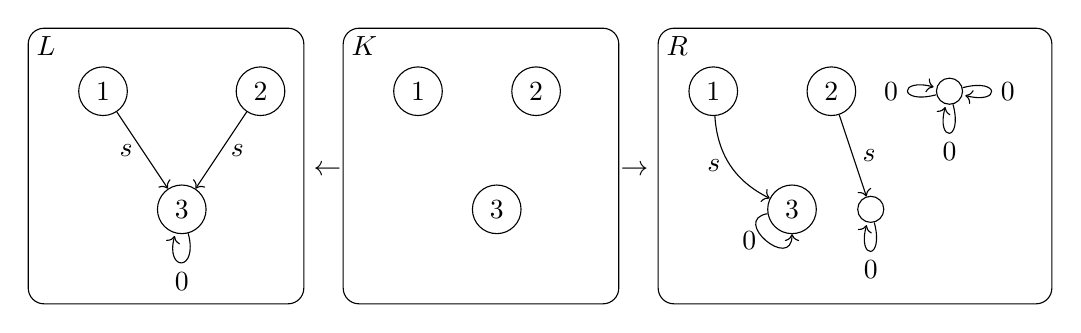
\begin{tikzpicture}
                \graphbox{$L$}{0mm}{0mm}{35mm}{35mm}{2mm}{-5mm}{
                    \coordinate (delta) at (0,-18mm);
                    \node[draw,circle] (l1) at ($(delta)+(-1,1.5)$) {1};
                    \node[draw,circle] (l2) at ($(delta)+(1,1.5)$) {2};
                    \node[draw,circle] (l3) at ($(delta)+(0,0)$) {3};
                    \draw[->] (l1) -- (l3) node[midway,left] {$s$};
                    \draw[->] (l2) -- (l3) node[midway,right] {$s$};
                    \draw[->] (l3) edge [loop below] node {0} (l3);
                }
                    \graphbox{$K$}{40mm}{0mm}{35mm}{35mm}{2mm}{-5mm}{
                        \coordinate (delta) at (0,-18mm);
                        \coordinate (interfaceorigin) at ($(delta) +(5,0)$);
                        \node[draw,circle] (r1) at ($(delta) +(-1,1.5)$) {1};
                        \node[draw,circle] (r2) at ($(delta) +(0.5,1.5)$) {2};
                        \node[draw,circle] (r3) at ($(delta)+(0,0)$) {3};
                    } 
                    \node () at (38mm,-18mm) {$\leftarrow$};
                    \node () at (77mm,-18mm) {$\rightarrow$};
                \graphbox{$R$}{80mm}{0mm}{50mm}{35mm}{2mm}{-5mm}{
                    \coordinate (delta) at (-10mm,-18mm);
                    \node[draw,circle] (r1) at ($(delta)+(-1,1.5)$) {1};
                    \node[draw,circle] (r2) at ($(delta)+(0.5,1.5)$) {2};
                    \node[draw,circle] (r3) at ($(delta)+(0,0)$) {3};
                    \node[draw,circle] (r4) at ($(delta)+(1,0)$) {};
                    \draw[->] (r1) edge[bend right] node[midway,left] {$s$} (r3) ;
                    \draw[->] (r2) -- (r4) node[midway,right] {$s$};
                    \draw[->] (r4) edge [loop below] node {0} (r4);
                    
                    \draw[->] (r3) edge [out=190,in=270,looseness=3] node[midway,left] {0} (r3);
                    \node[draw,circle] (r5) at ($(r2)+(1.5,0)$) {};
                    \draw[->] (r5) edge [loop below] node {0} (r5);
                    \draw[->] (r5) edge [loop right] node {0} (r5);
                    \draw[->] (r5) edge [loop left] node {0} (r5);
                }
            \end{tikzpicture}
            }
    \end{center}
All existing automated methods fail.

 Intuition: the number of morphisms from $\tikz[baseline=-0.5ex]{ 
                \node (x) at (0,0) {$\bullet$}; 
                \node (y) at (1,0) {$\bullet$};
                \node (z) at (2,0) {$\bullet$};
                \draw[->] (x) -- (y) node[midway, above] {$s$};
                \draw[->] (z) -- (y) node[midway, above] {$s$};
 }$ strictly decreases.
\end{frame}

\section{Toward greater power}
\begin{frame}
  \tableofcontents[currentsection,hideothersubsections]
\end{frame}

\begin{frame}{Morphism Counting}
    Termination by interpretation 
    \newline\newline
    Parameter: a graph $X$
    \newline\newline
    Interpretation of a graph $G$ : number of morphisms from $X$ to $G$
\end{frame}

\begin{frame}{Inclusions: morphisms $h$ with $h(x) = x$ for all $x$.}
         \begin{center} 
            \resizebox{\textwidth}{!}{
                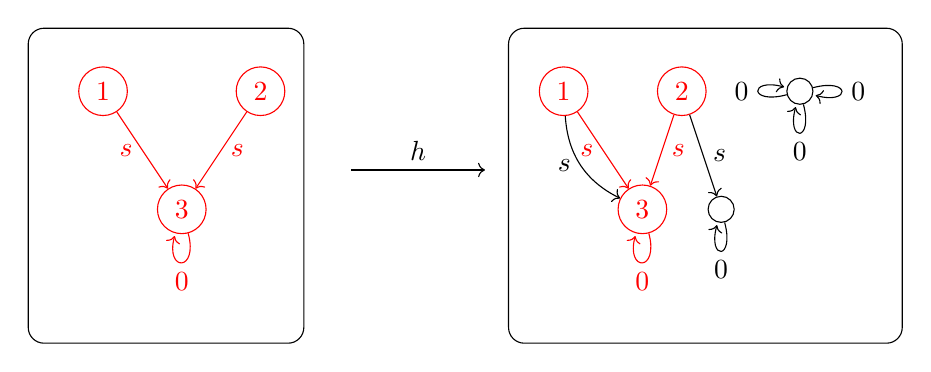
\begin{tikzpicture}
                    \graphbox{}{39mm}{0mm}{35mm}{40mm}{2mm}{-5mm}{
                        \coordinate (delta) at (0,-18mm);
                        \node[draw,circle,red] (l1) at ($(delta)+(-1,1.5)$) {1};
                        \node[draw,circle,red] (l2) at ($(delta)+(1,1.5)$) {2};
                        \node[draw,circle,red] (l3) at ($(delta)+(0,0)$) {3};
                        \draw[->,red] (l1) -- (l3) node[midway,left] {$s$};
                        \draw[->,red] (l2) -- (l3) node[midway,right] {$s$};
                        \draw[->,red] (l3) edge [loop below] node {0} (l3);
                    }
                        \draw[->] (80mm,-18mm) to node[midway,above] {$h$} (97mm,-18mm);
                    \graphbox{}{100mm}{0mm}{50mm}{40mm}{2mm}{-5mm}{
                        \coordinate (delta) at (-10mm,-18mm);
                        \node[draw,circle,red] (r1) at ($(delta)+(-1,1.5)$) {1};
                        \node[draw,circle,red] (r2) at ($(delta)+(0.5,1.5)$) {2};
                        \node[draw,circle,red] (r3) at ($(delta)+(0,0)$) {3};
                        \node[draw,circle] (r4) at ($(delta)+(1,0)$) {};
                        \node[draw,circle] (r5) at ($(r2)+(1.5,0)$) {};
                        \draw[->] (r1) edge[bend right] node[midway,left] {$s$} (r3) ; 
                        \draw[->] (r2) -- (r4) node[midway,right] {$s$};
                        \draw[->] (r4) edge [loop below] node {0} (r4);
                        \draw[->] (r5) edge [loop below] node {0} (r5);
                        \draw[->] (r5) edge [loop right] node {0} (r5);
                        \draw[->] (r5) edge [loop left] node {0} (r5);
                        \draw[->,red] (r1) edge node[midway,left] {$s$} (r3) ;
                        \draw[->,red] (r2) edge node[midway,right] {$s$} (r3) ; 
                        \draw[->,red] (r3) edge [loop below] node {0} (r3); 
                    }
                \end{tikzpicture}
                }
        \end{center}
 Subgraph
 
\end{frame}

% \begin{frame}{Graph rewriting rule}
%       \begin{beamercolorbox}[rounded=true,shadow=true,wd=\textwidth]{block body}
%         \textcolor{blue}{Rules} $\varphi \mathop{=} (L \overset{l}{\leftarrow} K \overset{r}{\rightarrow} R)$ consist of inclusions $l$ and $r$. 
%       \end{beamercolorbox}
%     \begin{center} 
%         \resizebox{\textwidth}{!}{
%         $\alpha$ = 
%         \begin{tikzpicture}[baseline=-10mm]
%             \graphbox{\( L \)}{0mm}{-3mm}{34mm}{12mm}{2mm}{2mm}{
%                 \coordinate (o) at (0mm,-8mm); 
%                 \node[draw,circle] (l1) at ($(o)+(-10mm,0mm)$) {1};
%                 \node[draw,circle] (l2) at ($(l1)+(2,0)$) {2};
%                 \node[draw,circle] (l3) at ($(l1)+(1,0)$) {3};
%                 \draw[->] (l1) -- (l3) node[midway,above] {$a$};
%                 \draw[->] (l3) -- (l2) node[midway,above] {$a$};
%             } 

%             \graphbox{\( K \)}{40mm}{-3mm}{34mm}{12mm}{2mm}{2mm}{
%                 \coordinate (o) at (0mm,-8mm); 
%                 \node[draw,circle] (l1) at ($(o)+(-10mm,0mm)$) {1};
%                 \node[draw,circle] (l2) at ($(l1)+(2,0)$) {2};
%             }  

%             \graphbox{\( R \)}{80mm}{-3mm}{45mm}{12mm}{2mm}{2mm}{
%                 \coordinate (o) at (-5mm,-8mm); 
%                 \node[draw,circle] (l1) at ($(o)+(-10mm,0mm)$) {1};
%                 \node[draw,circle] (l2) at ($(l1)+(3,0)$) {2};
%                 \node[draw,circle] (l3) at ($(l1)+(1,0)$) {4};
%                 \node[draw,circle] (l4) at ($(l1)+(2,0)$) {5};
%                 \draw[->] (l1) -- (l3) node[midway,above] {$a$};
%                 \draw[->] (l3) -- (l4) node[midway,above] {$b$};
%                 \draw[->] (l4) -- (l2) node[midway,above] {$a$};
%             }    
%             \node () at (37mm,-8mm) {\( \overset{l}{\leftarrow} \)}; % K -> L
%             \node () at (77mm,-8mm) {\( \overset{r}{\rightarrow} \)}; % K -> R
%         \end{tikzpicture}
%         } 
%     \end{center}   
% % to do todo
%             \begin{beamercolorbox}[rounded=true,shadow=true,wd=\textwidth]{block body}
%             Rule $\varphi' \mathop{=} (L' \overset{l'}{\leftarrow} K' \overset{r'}{\rightarrow} R')$ and $\varphi$ are \textcolor{blue}{equivalent} if 
%             there are isomorphisms $a,b,c$ such that:
%             \begin{center} 
%                     \resizebox{0.40\textwidth}{!}{
%                         \begin{tikzpicture}
%                                 \node (I) at (0,-0.7) {$K'$};
%                                 \node (L) at (-2,-0.7) {$L'$};
%                                 \node (R) at (2,-0.7) {$R'$};
%                                 \node (G) at (-2,-2) {$L$};
%                                 \node (C) at (0,-2) {$K$};
%                                 \node (H) at (2,-2) {$R$};
%                                 \draw [->] (I) to  node [midway,above] {$l'$} (L);
%                                 \draw [->] (I) to  node [midway,above] {$r'$} (R);
%                                 \draw [->] (L) to node [midway,right] {$a$} (G);
%                                 \draw [->] (I) to node [midway,right] {$b$} (C);
%                                 \draw [->] (R) to node [midway,left] {$c$} (H);
%                                 \draw [->] (C) to node [midway,above] {$l$} (G);
%                                 \draw [->] (C) to node [midway,above] {$r$} (H);
%                                 \node [at=($(I)!.5!(G)$)] {=};
%                                 \node [at=($(I)!.5!(H)$)] {=};
%                             \end{tikzpicture}
%                     }
%                 \end{center}
%         \end{beamercolorbox}
%     \begin{center}
%      \resizebox{\textwidth}{!}{
%         $\alpha'$ = 
%            \begin{tikzpicture}[baseline=-10mm]
%                 \graphbox{\( L' \)}{0mm}{-3mm}{34mm}{12mm}{2mm}{2mm}{
%                     \coordinate (o) at (0mm,-8mm); 
%                     \node[draw,circle] (l1) at ($(o)+(-10mm,0mm)$) {6};
%                     \node[draw,circle] (l2) at ($(l1)+(2,0)$) {8};
%                     \node[draw,circle] (l3) at ($(l1)+(1,0)$) {7};
%                     \draw[->] (l1) -- (l3) node[midway,above] {$a$};
%                     \draw[->] (l3) -- (l2) node[midway,above] {$a$};
%                 } 
        
%                 \graphbox{\( K' \)}{40mm}{-3mm}{34mm}{12mm}{2mm}{2mm}{
%                     \coordinate (o) at (0mm,-8mm); 
%                     \node[draw,circle] (l1) at ($(o)+(-10mm,0mm)$) {6};
%                     \node[draw,circle] (l2) at ($(l1)+(2,0)$) {7};
%                 }  
        
%                 \graphbox{\( R' \)}{80mm}{-3mm}{45mm}{12mm}{2mm}{2mm}{
%                     \coordinate (o) at (-5mm,-8mm); 
%                     \node[draw,circle] (l1) at ($(o)+(-10mm,0mm)$) {6};
%                     \node[draw,circle] (l2) at ($(l1)+(3,0)$) {7};
%                     \node[draw,circle] (l3) at ($(l1)+(1,0)$) {9};
%                     \node[draw,circle] (l4) at ($(l1)+(2,0)$) {10};
%                     \draw[->] (l1) -- (l3) node[midway,above] {$a$};
%                     \draw[->] (l3) -- (l4) node[midway,above] {$b$};
%                     \draw[->] (l4) -- (l2) node[midway,above] {$a$};
%                 }    
%                 \node () at (37mm,-8mm) {\( \overset{l'}{\leftarrow} \)};  
%                 \node () at (77mm,-8mm) {\( \overset{r'}{\rightarrow} \)}; %
%             \end{tikzpicture}
%             }     
%     \end{center}    
% \end{frame}

% \begin{frame}{Graph Rewriting}
 
%  Rewriting steps $G \mathop{\Rightarrow}_\varphi H$ using rule $\varphi$ are commutative diagrams with an equivalent rule $L' \overset{l'}{\leftarrow} K' \overset{r'}{\rightarrow} R'$ where all morphisms are inclusions:
%          \begin{center}
%           \resizebox{0.40\textwidth}{!}{
%               \begin{tikzpicture}
%                     \node (I) at (0,-0.7) {$K'$};
%                     \node (L) at (-2,-0.7) {$L'$};
%                     \node (R) at (2,-0.7) {$R'$};
%                     \node (G) at (-2,-2) {$G$};
%                     \node (C) at (0,-2) {$C$};
%                     \node (H) at (2,-2) {$H$};
%                     \draw [->] (I) to  node [midway,below] {$l'$} (L);
%                     \draw [->] (I) to  node [midway,below] {$r'$} (R);
%                     \draw [->] (L) to node [midway,left] {} (G);
%                     \draw [->] (I) to node [midway,right] { } (C);
%                     \draw [->] (R) to node [midway,left] { } (H);
%                     \draw [->] (C) to node [midway,above] { } (G);
%                     \draw [->] (C) to node [midway,above] { } (H);
%                     \node [at=($(I)!.5!(G)$)] {} ;
%                     \node [at=($(I)!.5!(H)$)] {};
%                   \end{tikzpicture}
%           }
%       \end{center}
% \end{frame} 
 
\begin{frame}{Graph Rewriting with Injective Rules}
  A rewriting rules consists of two inclusions. 
  \begin{center}
    $\varphi$=\resizebox{0.78\textwidth}{!}{
      \begin{tikzpicture}[baseline=-10mm]
              \graphbox{\( L\)}{0mm}{5mm}{34mm}{15mm}{2mm}{0mm}{
                  \coordinate (o) at (0mm,-8mm); 
                  \node[draw,circle] (l1) at ($(o)+(-10mm,0mm)$) {6};
                  \node[draw,circle] (l2) at ($(l1)+(2,0)$) {7};
                  \node[orange,draw,circle] (l3) at ($(l1)+(1,0)$) {8};
                  \draw[orange,->] (l1) -- (l3) node[midway,above] {$a$};
                  \draw[orange,->] (l3) -- (l2) node[midway,above] {$a$};
              } 

              \graphbox{\( K \)}{40mm}{5mm}{34mm}{15mm}{2mm}{0mm}{
                  \coordinate (o) at (0mm,-8mm); 
                  \node[draw,circle] (l1) at ($(o)+(-10mm,0mm)$) {6};
                  \node[draw,circle] (l2) at ($(l1)+(2,0)$) {7};
              }  

              \graphbox{\( R \)}{80mm}{5mm}{45mm}{15mm}{2mm}{0mm}{
                  \coordinate (o) at (-5mm,-8mm); 
                  \node[draw,circle] (l1) at ($(o)+(-10mm,0mm)$) {6};
                  \node[draw,circle] (l2) at ($(l1)+(3,0)$) {7};
                  \node[red,draw,circle] (l3) at ($(l1)+(1,0)$) {9};
                  \node[red,draw,circle] (l4) at ($(l1)+(2,0)$) {10};
                  \draw[red,->] (l1) -- (l3) node[midway,above] {$a$};
                  \draw[red,->] (l3) -- (l4) node[midway,above] {$b$};
                  \draw[red,->] (l4) -- (l2) node[midway,above] {$a$};
              }    
              \node () at (37mm,-3mm) {\( \overset{l}{\leftarrow} \)}; % K -> L
              \node () at (77mm,-3mm) {\( \overset{r}{\rightarrow} \)}; % K -> R
      \end{tikzpicture}
      }
   \end{center}

   An equivalent rewriting rule expresses the same transformation. 

  \begin{center}
    $\varphi'$=\resizebox{0.78\textwidth}{!}{
      \begin{tikzpicture}[baseline=-10mm]
              \graphbox{\( L' \)}{0mm}{5mm}{34mm}{15mm}{2mm}{0mm}{
                  \coordinate (o) at (0mm,-8mm); 
                  \node[draw,circle] (l1) at ($(o)+(-10mm,0mm)$) {1};
                  \node[draw,circle] (l2) at ($(l1)+(2,0)$) {2};
                  \node[orange,draw,circle] (l3) at ($(l1)+(1,0)$) {3};
                  \draw[orange,->] (l1) -- (l3) node[midway,above] {$a$};
                  \draw[orange,->] (l3) -- (l2) node[midway,above] {$a$};
              } 

              \graphbox{\( K' \)}{40mm}{5mm}{34mm}{15mm}{2mm}{0mm}{
                  \coordinate (o) at (0mm,-8mm); 
                  \node[draw,circle] (l1) at ($(o)+(-10mm,0mm)$) {1};
                  \node[draw,circle] (l2) at ($(l1)+(2,0)$) {2};
              }  

              \graphbox{\( R' \)}{80mm}{5mm}{45mm}{15mm}{2mm}{0mm}{
                  \coordinate (o) at (-5mm,-8mm); 
                  \node[draw,circle] (l1) at ($(o)+(-10mm,0mm)$) {1};
                  \node[draw,circle] (l2) at ($(l1)+(3,0)$) {2};
                  \node[red,draw,circle] (l3) at ($(l1)+(1,0)$) {4};
                  \node[red,draw,circle] (l4) at ($(l1)+(2,0)$) {5};
                  \draw[red,->] (l1) -- (l3) node[midway,above] {$a$};
                  \draw[red,->] (l3) -- (l4) node[midway,above] {$b$};
                  \draw[red,->] (l4) -- (l2) node[midway,above] {$a$};
              }    
              \node () at (37mm,-3mm) {\( \overset{l'}{\leftarrow} \)}; 
              \node () at (77mm,-3mm) {\( \overset{r'}{\rightarrow} \)}; 
      \end{tikzpicture}
      }
   \end{center}
  
   A rewriting step with $\varphi$ is defined by a DPO diagram with inclusions and $\varphi'$.
  \begin{center}
    \resizebox{0.78\textwidth}{!}{
      \begin{tikzpicture}
              \graphbox{\( L' \)}{0mm}{5mm}{34mm}{15mm}{2mm}{0mm}{
                  \coordinate (o) at (0mm,-8mm); 
                  \node[draw,circle] (l1) at ($(o)+(-10mm,0mm)$) {1};
                  \node[draw,circle] (l2) at ($(l1)+(2,0)$) {2};
                  \node[orange,draw,circle] (l3) at ($(l1)+(1,0)$) {3};
                  \draw[orange,->] (l1) -- (l3) node[midway,above] {$a$};
                  \draw[orange,->] (l3) -- (l2) node[midway,above] {$a$};
              } 

              \graphbox{\( K' \)}{40mm}{5mm}{34mm}{15mm}{2mm}{0mm}{
                  \coordinate (o) at (0mm,-8mm); 
                  \node[draw,circle] (l1) at ($(o)+(-10mm,0mm)$) {1};
                  \node[draw,circle] (l2) at ($(l1)+(2,0)$) {2};
              }  

              \graphbox{\( R' \)}{80mm}{5mm}{45mm}{15mm}{2mm}{0mm}{
                  \coordinate (o) at (-5mm,-8mm); 
                  \node[draw,circle] (l1) at ($(o)+(-10mm,0mm)$) {1};
                  \node[draw,circle] (l2) at ($(l1)+(3,0)$) {2};
                  \node[red,draw,circle] (l3) at ($(l1)+(1,0)$) {4};
                  \node[red,draw,circle] (l4) at ($(l1)+(2,0)$) {5};
                  \draw[red,->] (l1) -- (l3) node[midway,above] {$a$};
                  \draw[red,->] (l3) -- (l4) node[midway,above] {$b$};
                  \draw[red,->] (l4) -- (l2) node[midway,above] {$a$};
              }    
                \graphbox{\( G  \)}{0mm}{-17mm}{34mm}{25mm}{2mm}{-5mm}{
                  \coordinate (o) at (0mm,-3mm); 
                  \node[draw,circle] (l1) at ($(o)+(-10mm,0mm)$) {1};
                  \node[draw,circle] (l2) at ($(l1)+(2,0)$) {2};
                  \node[draw,circle,orange] (l3) at ($(l1)+(1,0)$) {3};
                  \node[blue, draw,circle] (l4) at ($(l2)+(0,-1)$) {6};
                  \draw[orange,->] (l1) -- (l3) node[midway,above] {$a$};
                  \draw[orange,->] (l3) -- (l2) node[midway,above] {$a$};
                  \draw[blue,->] (l2) -- (l4) node[midway,right] {$a$};
              }    
              \graphbox{\( C  \)}{40mm}{-17mm}{34mm}{25mm}{2mm}{-5mm}{
                  \coordinate (o) at (0mm,-3mm); 
                  \node[draw,circle] (l1) at ($(o)+(-10mm,0mm)$) {1};
                  \node[draw,circle] (l2) at ($(l1)+(2,0)$) {2};
                  \node[blue,draw,circle] (l4) at ($(l2)+(0,-1)$) {6};
                  \draw[blue,->] (l2) -- (l4) node[midway,right] {$a$};
              }    
              \graphbox{\( H   \)}{80mm}{-17mm}{45mm}{25mm}{2mm}{-5mm}{
                  \coordinate (o) at (-5mm,-3mm); 
                  \node[draw,circle] (l1) at ($(o)+(-10mm,0mm)$) {1};
                  \node[draw,circle] (l2) at ($(l1)+(3,0)$) {2};
                  \node[draw,circle,red] (l3) at ($(l1)+(1,0)$) {4};
                  \node[draw,circle,red] (l4) at ($(l1)+(2,0)$) {5};
                  \node[blue,draw,circle] (l5) at ($(l2)+(0,-1)$) {6};
                  \draw[red,->] (l1) -- (l3) node[midway,above] {$a$};
                  \draw[red,->] (l3) -- (l4) node[midway,above] {$b$};
                  \draw[red,->] (l4) -- (l2) node[midway,above] {$a$};
                  \draw[blue,->] (l2) -- (l5) node[midway,right] {$a$};
              }    
              \node () at (37mm,-3mm) {\( \overset{l'}{\leftarrow} \)}; 
              \node () at (77mm,-3mm) {\( \overset{r'}{\rightarrow} \)}; 
              \node () at (17mm,-13mm) {\( \downarrow \)};
              \node () at (37mm,-28mm) {\( \leftarrow \)};
              \node () at (52mm,-13mm) {\( \downarrow \)};
              \node () at (92mm,-13mm) {\( \downarrow \)};
              \node () at (77mm,-28mm) {\( \rightarrow \)};  
      \end{tikzpicture}
      }
   \end{center}
\end{frame}

\begin{frame}{Pre-Graphs}
  \noindent Graph:
         \begin{center}
            \resizebox{0.5\textwidth}{!}{
            \begin{tikzpicture}
                \graphbox{}{0mm}{-20mm}{45mm}{20mm}{5mm}{-3mm}{ 
                    \coordinate (o) at (-5mm,-8mm); 
                    \node[draw,circle] (l1) at ($(o)+(-10mm,0mm)$) {1};
                    \node[draw,circle] (l3) at ($(l1)+(1,0)$) {2};
                    \node[draw,circle] (l4) at ($(l1)+(2,0)$) {3};
                    \draw[->] (l1) edge[bend right]  node[midway,below] {$a$} (l3);
                    \draw[->] (l1) edge[bend left] node[midway,above] {$a$}  (l3);
                    \draw[->] (l3) -- (l4) node[midway,above] {$b$};
                }  
            \end{tikzpicture} 
        }
        \end{center} 
    \begin{beamercolorbox}[rounded=true,shadow=true,wd=\textwidth]{block body}
    \noindent Pre-graphs obtained by removing node 2:
    \end{beamercolorbox}
        \begin{center}
            \resizebox{0.5\textwidth}{!}{
            \begin{tikzpicture}
                \graphbox{}{0mm}{-20mm}{45mm}{20mm}{5mm}{-3mm}{ 
                    \coordinate (o) at (-5mm,-8mm); 
                    \node[draw,circle] (l1) at ($(o)+(-10mm,0mm)$) {1};
                    \node[draw,circle,dashed,red] (l3) at ($(l1)+(1,0)$) {2};
                    \node[draw,circle] (l4) at ($(l1)+(2,0)$) {3};
                    \draw[->] (l1) edge[bend right]  node[midway,below] {$a$} (l3);
                    \draw[->] (l1) edge[bend left] node[midway,above] {$a$}  (l3);
                    \draw[->] (l3) -- (l4) node[midway,above] {$b$};
                }  
            \end{tikzpicture} 
        }
        \end{center} 

    \begin{description}
      \item All edges are dangling.
      % \item 2 existing nodes: 1 and 3.
    \end{description}
\end{frame}

\begin{frame}{Pre-Graph Operations}
     \begin{beamercolorbox}[rounded=true,shadow=true,wd=\textwidth]{block body}
        \textcolor{red}{Union} of two pre-graphs $C \mathop{\subseteq} G$ and $R \mathop{\subseteq} G$, denoted $C \mathop{\cup} R$.
    \end{beamercolorbox}
\begin{center}
    \resizebox{\textwidth}{!}{
        \begin{tikzpicture}          
            \graphbox{\( C  \)}{0mm}{-22mm}{34mm}{25mm}{2mm}{-3mm}{
                \coordinate (o) at (0mm,-6mm); 
                \node[draw,circle,dashed] (l1) at ($(o)+(-10mm,0mm)$) {1};
                \node[draw,circle,dashed] (l2) at ($(l1)+(2,0)$) {2};
                \node[draw,circle] (l4) at ($(l2)+(0,-1)$) {6};
                \draw[->] (l2) -- (l4) node[midway,right] {$a$};
            }     
            \graphbox{\( R \)}{40mm}{-22mm}{45mm}{25mm}{2mm}{2mm}{
                \coordinate (o) at (-5mm,-8mm); 
                \node[draw,circle] (l1) at ($(o)+(-10mm,0mm)$) {1};
                \node[draw,circle] (l2) at ($(l1)+(3,0)$) {2};
                \node[draw,circle] (l3) at ($(l1)+(1,0)$) {4};
                \node[draw,circle] (l4) at ($(l1)+(2,0)$) {5};
                \draw[->] (l1) -- (l3) node[midway,above] {$a$};
                \draw[->] (l3) -- (l4) node[midway,above] {$b$};
                \draw[->] (l4) -- (l2) node[midway,above] {$a$};
            } 
            \graphbox{\textcolor{red}{\(C \mathop{\cup} R \)}}{91mm}{-22mm}{45mm}{25mm}{2mm}{-3mm}{
                \coordinate (o) at (-5mm,-6mm); 
                \node[draw,circle] (l1) at ($(o)+(-10mm,0mm)$) {1};
                \node[draw,circle] (l2) at ($(l1)+(3,0)$) {2};
                \node[draw,circle] (l3) at ($(l1)+(1,0)$) {4};
                \node[draw,circle] (l4) at ($(l1)+(2,0)$) {5};
                \node[ draw,circle] (l5) at ($(l2)+(0,-1)$) {6};
                \draw[->] (l1) -- (l3) node[midway,above] {$a$};
                \draw[->] (l3) -- (l4) node[midway,above] {$b$};
                \draw[->] (l4) -- (l2) node[midway,above] {$a$};
                \draw[->] (l2) -- (l5) node[midway,right] {$a$};
            }    
             
        \end{tikzpicture}
    }
    \end{center}
 \begin{beamercolorbox}[rounded=true,shadow=true,wd=\textwidth]{block body}
     \textcolor{red}{Relative complement} of $R$ in $H$ where $R \mathop{\subseteq} H$, denoted $H \mathop{\setminus} R$.
\end{beamercolorbox}
    \begin{center} 
  \resizebox{\textwidth}{!}{
        \begin{tikzpicture}       
            \graphbox{\( H \)}{-11mm}{-22mm}{45mm}{25mm}{2mm}{-3mm}{
                \coordinate (o) at (-5mm,-6mm); 
                \node[draw,circle] (l1) at ($(o)+(-10mm,0mm)$) {1};
                \node[draw,circle] (l2) at ($(l1)+(3,0)$) {2};
                \node[draw,circle] (l3) at ($(l1)+(1,0)$) {4};
                \node[draw,circle] (l4) at ($(l1)+(2,0)$) {5};
                \node[ draw,circle] (l5) at ($(l2)+(0,-1)$) {6};
                \draw[-] (l1) -- (l3) node[midway,above] {$a$};
                \draw[-] (l3) -- (l4) node[midway,above] {$b$};
                \draw[-] (l4) -- (l2) node[midway,above] {$a$};
                \draw[-] (l2) -- (l5) node[midway,right] {$a$};
            }   
            \graphbox{\( R \)}{40mm}{-22mm}{45mm}{25mm}{2mm}{2mm}{
                \coordinate (o) at (-5mm,-8mm); 
                \node[draw,circle] (l1) at ($(o)+(-10mm,0mm)$) {1};
                \node[draw,circle] (l2) at ($(l1)+(3,0)$) {2};
                \node[draw,circle] (l3) at ($(l1)+(1,0)$) {4};
                \node[draw,circle] (l4) at ($(l1)+(2,0)$) {5};
                \draw[-] (l1) -- (l3) node[midway,above] {$a$};
                \draw[-] (l3) -- (l4) node[midway,above] {$b$};
                \draw[-] (l4) -- (l2) node[midway,above] {$a$};
            }     
            \graphbox{\textcolor{red}{\( H \mathop{\setminus} R  \)}}{90mm}{-22mm}{34mm}{25mm}{2mm}{-3mm}{
                \coordinate (o) at (0mm,-6mm); 
                \node[draw,dashed,circle] (l1) at ($(o)+(-10mm,0mm)$) {1};
                \node[draw,dashed,circle] (l2) at ($(l1)+(2,0)$) {2};
                \node[draw,circle] (l4) at ($(l2)+(0,-1)$) {6};
                \draw[-] (l2) -- (l4) node[midway,right] {$a$};
            }   
        \end{tikzpicture}
    }
    \end{center}
\end{frame}

% \begin{frame}{Decomposition of Graphs in Rewriting Steps}
%     \begin{center}
%     \resizebox{\textwidth}{!}{
%       \begin{tikzpicture}
%               \graphbox{\( L \mathop{=} L' \mathop{\cup} K \)}{0mm}{5mm}{34mm}{20mm}{2mm}{-5mm}{
%                   \coordinate (o) at (0mm,-8mm); 
%                   \node[draw,circle] (l1) at ($(o)+(-10mm,0mm)$) {1};
%                   \node[draw,circle] (l2) at ($(l1)+(2,0)$) {2};
%                   \node[orange,draw,circle] (l3) at ($(l1)+(1,0)$) {3};
%                   \draw[orange,->] (l1) -- (l3) node[midway,above] {$a$};
%                   \draw[orange,->] (l3) -- (l2) node[midway,above] {$a$};
%               } 

%               \graphbox{\( K \)}{40mm}{5mm}{34mm}{20mm}{2mm}{-5mm}{
%                   \coordinate (o) at (0mm,-8mm); 
%                   \node[draw,circle] (l1) at ($(o)+(-10mm,0mm)$) {1};
%                   \node[draw,circle] (l2) at ($(l1)+(2,0)$) {2};
%               }  

%               \graphbox{\( R \mathop{=} R' \mathop{\cup} K \)}{80mm}{5mm}{45mm}{20mm}{2mm}{-5mm}{
%                   \coordinate (o) at (-5mm,-8mm); 
%                   \node[draw,circle] (l1) at ($(o)+(-10mm,0mm)$) {1};
%                   \node[draw,circle] (l2) at ($(l1)+(3,0)$) {2};
%                   \node[red,draw,circle] (l3) at ($(l1)+(1,0)$) {4};
%                   \node[red,draw,circle] (l4) at ($(l1)+(2,0)$) {5};
%                   \draw[red,->] (l1) -- (l3) node[midway,above] {$a$};
%                   \draw[red,->] (l3) -- (l4) node[midway,above] {$b$};
%                   \draw[red,->] (l4) -- (l2) node[midway,above] {$a$};
%               }    

%               \graphbox{\( G \mathop{=} L' \mathop{\cup} K \mathop{\cup} C' \)}{0mm}{-22mm}{34mm}{30mm}{2mm}{-10mm}{
%                   \coordinate (o) at (0mm,-3mm); 
%                   \node[draw,circle] (l1) at ($(o)+(-10mm,0mm)$) {1};
%                   \node[draw,circle] (l2) at ($(l1)+(2,0)$) {2};
%                   \node[draw,circle,orange] (l3) at ($(l1)+(1,0)$) {3};
%                   \node[blue, draw,circle] (l4) at ($(l2)+(0,-1)$) {6};
%                   \draw[orange,->] (l1) -- (l3) node[midway,above] {$a$};
%                   \draw[orange,->] (l3) -- (l2) node[midway,above] {$a$};
%                   \draw[blue,->] (l2) -- (l4) node[midway,right] {$a$};
%               }    

%               \graphbox{\( C \mathop{=} K \mathop{\cup} C' \)}{40mm}{-22mm}{34mm}{30mm}{2mm}{-10mm}{
%                   \coordinate (o) at (0mm,-3mm); 
%                   \node[draw,circle] (l1) at ($(o)+(-10mm,0mm)$) {1};
%                   \node[draw,circle] (l2) at ($(l1)+(2,0)$) {2};
%                   \node[blue,draw,circle] (l4) at ($(l2)+(0,-1)$) {6};
%                   \draw[blue,->] (l2) -- (l4) node[midway,right] {$a$};
%               }    

%               \graphbox{\( H \mathop{=} R' \mathop{\cup} K \mathop{\cup} C' \)}{80mm}{-22mm}{45mm}{30mm}{2mm}{-10mm}{
%                   \coordinate (o) at (-5mm,-3mm); 
%                   \node[draw,circle] (l1) at ($(o)+(-10mm,0mm)$) {1};
%                   \node[draw,circle] (l2) at ($(l1)+(3,0)$) {2};
%                   \node[draw,circle,red] (l3) at ($(l1)+(1,0)$) {4};
%                   \node[draw,circle,red] (l4) at ($(l1)+(2,0)$) {5};
%                   \node[blue,draw,circle] (l5) at ($(l2)+(0,-1)$) {6};
%                   \draw[red,->] (l1) -- (l3) node[midway,above] {$a$};
%                   \draw[red,->] (l3) -- (l4) node[midway,above] {$b$};
%                   \draw[red,->] (l4) -- (l2) node[midway,above] {$a$};
%                   \draw[blue,->] (l2) -- (l5) node[midway,right] {$a$};
%               }    

%               \node () at (37mm,-8mm) {\( \leftarrow \)}; % K -> L
%               \node () at (77mm,-8mm) {\( \rightarrow \)}; % K -> R
%               \node () at (17mm,-18mm) {\( \downarrow \)};
%               \node () at (37mm,-33mm) {\( \leftarrow \)};
%               \node () at (52mm,-18mm) {\( \downarrow \)};
%               \node () at (92mm,-18mm) {\( \downarrow \)};
%               \node () at (77mm,-33mm) {\( \rightarrow \)}; % C -> H
%       \end{tikzpicture}
%       }
%    \end{center}
% \end{frame}


% \begin{frame}{Decomposition of Graphs in Rewriting Steps}
%     \begin{center}
%     \resizebox{\textwidth}{!}{
%       \begin{tikzpicture}
%               \graphbox{\( L \mathop{=} L' \mathop{\cup} K \)}{0mm}{5mm}{34mm}{20mm}{2mm}{-5mm}{
%                   \coordinate (o) at (0mm,-8mm); 
%                   \node[draw,circle] (l1) at ($(o)+(-10mm,0mm)$) {};
%                   \node[draw,circle] (l2) at ($(l1)+(2,0)$) {};
%                   \node[orange,fill=orange,draw,circle] (l3) at ($(l1)+(1,0)$) {};
%                   \draw[orange,fill=orange,->] (l1) -- (l3) node[midway,above] {$a$};
%                   \draw[orange,fill=orange,->] (l3) -- (l2) node[midway,above] {$a$};
%               } 

%               \graphbox{\( K \)}{40mm}{5mm}{34mm}{20mm}{2mm}{-5mm}{
%                   \coordinate (o) at (0mm,-8mm); 
%                   \node[draw,circle] (l1) at ($(o)+(-10mm,0mm)$) {};
%                   \node[draw,circle] (l2) at ($(l1)+(2,0)$) {};
%               }  

%               \graphbox{\( R \mathop{=} R' \mathop{\cup} K \)}{80mm}{5mm}{45mm}{20mm}{2mm}{-5mm}{
%                   \coordinate (o) at (-5mm,-8mm); 
%                   \node[draw,circle] (l1) at ($(o)+(-10mm,0mm)$) {};
%                   \node[draw,circle] (l2) at ($(l1)+(3,0)$) {};
%                   \node[red,fill=red,draw,circle] (l3) at ($(l1)+(1,0)$) {};
%                   \node[red,fill=red,draw,circle] (l4) at ($(l1)+(2,0)$) {};
%                   \draw[red,fill=red,->] (l1) -- (l3) node[midway,above] {$a$};
%                   \draw[red,fill=red,->] (l3) -- (l4) node[midway,above] {$b$};
%                   \draw[red,fill=red,->] (l4) -- (l2) node[midway,above] {$a$};
%               }    

%               \graphbox{\( G \mathop{=} L' \mathop{\cup} K \mathop{\cup} C' \)}{0mm}{-22mm}{34mm}{30mm}{2mm}{-10mm}{
%                   \coordinate (o) at (0mm,-3mm); 
%                   \node[draw,circle] (l1) at ($(o)+(-10mm,0mm)$) {};
%                   \node[draw,circle] (l2) at ($(l1)+(2,0)$) {};
%                   \node[draw,circle,orange,fill=orange] (l3) at ($(l1)+(1,0)$) {};
%                   \node[blue, fill=blue,draw,circle] (l4) at ($(l2)+(0,-1)$) {};
%                   \draw[orange,fill=orange,->] (l1) -- (l3) node[midway,above] {$a$};
%                   \draw[orange,fill=orange,->] (l3) -- (l2) node[midway,above] {$a$};
%                   \draw[blue,fill=blue,->] (l2) -- (l4) node[midway,right] {$a$};
%               }    

%               \graphbox{\( C \mathop{=} K \mathop{\cup} C' \)}{40mm}{-22mm}{34mm}{30mm}{2mm}{-10mm}{
%                   \coordinate (o) at (0mm,-3mm); 
%                   \node[draw,circle] (l1) at ($(o)+(-10mm,0mm)$) {};
%                   \node[draw,circle] (l2) at ($(l1)+(2,0)$) {};
%                   \node[blue,fill=blue,draw,circle] (l4) at ($(l2)+(0,-1)$) {};
%                   \draw[blue,fill=blue,->] (l2) -- (l4) node[midway,right] {$a$};
%               }    

%               \graphbox{\( H \mathop{=} R' \mathop{\cup} K \mathop{\cup} C' \)}{80mm}{-22mm}{45mm}{30mm}{2mm}{-10mm}{
%                   \coordinate (o) at (-5mm,-3mm); 
%                   \node[draw,circle] (l1) at ($(o)+(-10mm,0mm)$) {};
%                   \node[draw,circle] (l2) at ($(l1)+(3,0)$) {};
%                   \node[draw,fill=red,circle] (l3) at ($(l1)+(1,0)$) {};
%                   \node[draw,fill=red,circle] (l4) at ($(l1)+(2,0)$) {};
%                   \node[blue,fill=blue,draw,circle] (l5) at ($(l2)+(0,-1)$) {};
%                   \draw[red,fill=red,->] (l1) -- (l3) node[midway,above] {$a$};
%                   \draw[red,fill=red,->] (l3) -- (l4) node[midway,above] {$b$};
%                   \draw[red,fill=red,->] (l4) -- (l2) node[midway,above] {$a$};
%                   \draw[blue,fill=blue,->] (l2) -- (l5) node[midway,right] {$a$};
%               }    

%               \node () at (37mm,-8mm) {\( \leftarrow \)}; % K -> L
%               \node () at (77mm,-8mm) {\( \rightarrow \)}; % K -> R
%               \node () at (17mm,-18mm) {\( \downarrow \)};
%               \node () at (37mm,-33mm) {\( \leftarrow \)};
%               \node () at (52mm,-18mm) {\( \downarrow \)};
%               \node () at (92mm,-18mm) {\( \downarrow \)};
%               \node () at (77mm,-33mm) {\( \rightarrow \)}; % C -> H
%       \end{tikzpicture}
%       }
%    \end{center}
% \end{frame}
\begin{frame}{Decomposition of Graphs in Rewriting Steps}
   \begin{center}
    \resizebox{0.8\textwidth}{!}{
      \begin{tikzpicture}
              \graphbox{\( L \mathop{=} L' \mathop{\cup} K \)}{0mm}{5mm}{34mm}{20mm}{2mm}{-5mm}{
                  \coordinate (o) at (0mm,-8mm); 
                  \node[draw,circle] (l1) at ($(o)+(-10mm,0mm)$) {};
                  \node[draw,circle] (l2) at ($(l1)+(2,0)$) {};
                  \node[orange,fill=orange,draw,circle] (l3) at ($(l1)+(1,0)$) {};
                  \draw[orange,fill=orange,->] (l1) -- (l3) node[midway,above] {$a$};
                  \draw[orange,fill=orange,->] (l3) -- (l2) node[midway,above] {$a$};
              } 

              \graphbox{\( K \)}{40mm}{5mm}{34mm}{20mm}{2mm}{-5mm}{
                  \coordinate (o) at (0mm,-8mm); 
                  \node[draw,circle] (l1) at ($(o)+(-10mm,0mm)$) {};
                  \node[draw,circle] (l2) at ($(l1)+(2,0)$) {};
              }  

              \graphbox{\( R \mathop{=} R' \mathop{\cup} K \)}{80mm}{5mm}{45mm}{20mm}{2mm}{-5mm}{
                  \coordinate (o) at (-5mm,-8mm); 
                  \node[draw,circle] (l1) at ($(o)+(-10mm,0mm)$) {};
                  \node[draw,circle] (l2) at ($(l1)+(3,0)$) {};
                  \node[red,fill=red,draw,circle] (l3) at ($(l1)+(1,0)$) {};
                  \node[red,fill=red,draw,circle] (l4) at ($(l1)+(2,0)$) {};
                  \draw[red,fill=red,->] (l1) -- (l3) node[midway,above] {$a$};
                  \draw[red,fill=red,->] (l3) -- (l4) node[midway,above] {$b$};
                  \draw[red,fill=red,->] (l4) -- (l2) node[midway,above] {$a$};
              }    

              \graphbox{\( G \mathop{=} L' \mathop{\cup} K \mathop{\cup} C' \)}{0mm}{-22mm}{34mm}{30mm}{2mm}{-10mm}{
                  \coordinate (o) at (0mm,-3mm); 
                  \node[draw,circle] (l1) at ($(o)+(-10mm,0mm)$) {};
                  \node[draw,circle] (l2) at ($(l1)+(2,0)$) {};
                  \node[draw,circle,orange,fill=orange] (l3) at ($(l1)+(1,0)$) {};
                  \node[blue, fill=blue,draw,circle] (l4) at ($(l2)+(0,-1)$) {};
                  \draw[orange,fill=orange,->] (l1) -- (l3) node[midway,above] {$a$};
                  \draw[orange,fill=orange,->] (l3) -- (l2) node[midway,above] {$a$};
                  \draw[blue,fill=blue,->] (l2) -- (l4) node[midway,right] {$a$};
              }    

              \graphbox{\( C \mathop{=} K \mathop{\cup} C' \)}{40mm}{-22mm}{34mm}{30mm}{2mm}{-10mm}{
                  \coordinate (o) at (0mm,-3mm); 
                  \node[draw,circle] (l1) at ($(o)+(-10mm,0mm)$) {};
                  \node[draw,circle] (l2) at ($(l1)+(2,0)$) {};
                  \node[blue,fill=blue,draw,circle] (l4) at ($(l2)+(0,-1)$) {};
                  \draw[blue,fill=blue,->] (l2) -- (l4) node[midway,right] {$a$};
              }    

              \graphbox{\( H \mathop{=} R' \mathop{\cup} K \mathop{\cup} C' \)}{80mm}{-22mm}{45mm}{30mm}{2mm}{-10mm}{
                  \coordinate (o) at (-5mm,-3mm); 
                  \node[draw,circle] (l1) at ($(o)+(-10mm,0mm)$) {};
                  \node[draw,circle] (l2) at ($(l1)+(3,0)$) {};
                  \node[red,fill=red,draw,circle] (l3) at ($(l1)+(1,0)$) {};
                  \node[red,fill=red,draw,circle] (l4) at ($(l1)+(2,0)$) {};
                  \node[blue,fill=blue,draw,circle] (l5) at ($(l2)+(0,-1)$) {};
                  \draw[red,fill=red,->] (l1) -- (l3) node[midway,above] {$a$};
                  \draw[red,fill=red,->] (l3) -- (l4) node[midway,above] {$b$};
                  \draw[red,fill=red,->] (l4) -- (l2) node[midway,above] {$a$};
                  \draw[blue,fill=blue,->] (l2) -- (l5) node[midway,right] {$a$};
              }    

              \node () at (37mm,-8mm) {\( \leftarrow \)}; % K -> L
              \node () at (77mm,-8mm) {\( \rightarrow \)}; % K -> R
              \node () at (17mm,-18mm) {\( \downarrow \)};
              \node () at (37mm,-33mm) {\( \leftarrow \)};
              \node () at (52mm,-18mm) {\( \downarrow \)};
              \node () at (92mm,-18mm) {\( \downarrow \)};
              \node () at (77mm,-33mm) {\( \rightarrow \)}; % C -> H
      \end{tikzpicture}
      }
   \end{center}
\begin{center}
    \resizebox{0.45\textwidth}{!}{
            \begin{tikzpicture} 
                \coordinate (k) at (0, 0);
                \draw[fill=white] ($(k)+(0,0)$) rectangle ($(k)+(0.5,0.5)$);
                \node () at ($(k)+(0.25,0.25)$) {\( \mathrm{K} \)};
            
                \coordinate (c) at (0, -2.2);
                \draw[fill=blue!30]
                ($(c)+(0,-0.5)$)
                -- ($(c)+(0,0.5)$) 
                -- ($(c)+(1,0.5)$) 
                arc[start angle=0, end angle=-90, radius=1]
                -- cycle;
                \node () at ($(c)+(0.75,0.25)$) {\( \mathrm{C'} \)};
                \draw[fill=white] ($(c)+(0,0)$) rectangle ($(c)+(0.5,0.5)$);
                \node () at ($(c)+(0.25,0.25)$) {\( \mathrm{K} \)};
            
                \coordinate (l) at (-3, 0);
                \draw[fill=orange!30] ($(l)+(-0.5,0)$) rectangle ($(l)+(0.5,1)$);
                \node () at ($(l)+(-0.23,0.25)$) {\( \mathrm{L'} \)};
                \draw[fill=white] ($(l)+(0,0)$) rectangle ($(l)+(0.5,0.5)$);
                \node () at ($(l)+(0.25,0.25)$) {\( \mathrm{K} \)};
            
                \coordinate (g) at (-3, -2.2);
                \draw[fill=blue!30]
                ($(g)+(0,-0.5)$)
                -- ($(g)+(0,0.5)$)
                -- ($(g)+(1,0.5)$) 
                arc[start angle=0, end angle=-90, radius=1]
                -- cycle;
                \draw[fill=orange!30] ($(g)+(-0.5,0)$) rectangle ($(g)+(0.5,1)$);
                \node () at ($(g)+(0.75,0.25)$) {\( \mathrm{C'} \)};
                \node () at ($(g)+(-0.23,0.25)$) {\( \mathrm{L'} \)};
                \draw[fill=white] ($(g)+(0,0)$) rectangle ($(g)+(0.5,0.5)$);
                \node () at ($(g)+(0.25,0.25)$) {\( \mathrm{K} \)};
            
                \coordinate (r) at (3,0);
                \draw[fill=red!30] ($(r)+(-0.5,0)$)
                -- ($(r)+(-0.5,0.5)$)
                -- ($(r)+(0,1)$)
                --  ($(r)+(0.5,1)$)
                -- ($(r)+(0.5,0)$)
                -- cycle;
                \node () at ($(r)+(-0.23,0.25)$) {\( \mathrm{R'} \)};
                \draw[fill=white] ($(r)+(0,0)$) rectangle ($(r)+(0.5,0.5)$);
                \node () at ($(r)+(0.25,0.25)$) {\( \mathrm{K} \)};
            
                \coordinate (h) at (3, -2.2);
                \draw[fill=blue!30]
                ($(h)+(0,-0.5)$)
                -- ($(h)+(0,0.5)$)
                -- ($(h)+(1,0.5)$) 
                arc[start angle=0, end angle=-90, radius=1]
                -- cycle;
                \draw[fill=red!30] ($(h)+(-0.5,0)$)
                -- ($(h)+(-0.5,0.5)$)
                -- ($(h)+(0,1)$)
                --  ($(h)+(0.5,1)$)
                -- ($(h)+(0.5,0)$)
                -- cycle;
            \node () at ($(h)+(0.75,0.25)$) {\( \mathrm{C'} \)};
            \draw[fill=white] ($(h)+(0,0)$) rectangle ($(h)+(0.5,0.5)$);
            \node () at ($(h)+(0.25,0.25)$) {\( \mathrm{K} \)};
            \node () at ($(h)+(-0.23,0.25)$) {\( \mathrm{R'} \)};
            
                \node[ font=\huge] (kl) at ($(k)!0.5!(l)+(0.25,0.25)$)
                {\( \leftarrow \)}
                ; 
                \node[ font=\huge] (kr) at ($(k)!0.5!(r)+(0.25,0.25)$)
                {\( \rightarrow \)}
                ;  
                \node[ font=\huge] (cg) at ($(c)!0.5!(g)+(0.25,0.25)$) 
                {\( \leftarrow \)}
            ;  
                \node[ font=\huge] (ch) at ($(c)!0.5!(h)+(0.25,0.25)$)
                {\( \rightarrow \)}
            ; 
                \node[ font=\huge] (kc) at ($(k)!0.5!(c)+(0.2,0.4)$) {\( \downarrow \)}; 
                \node[ font=\huge] (lg) at ($(l)!0.5!(g)+(0.1,0.4)$) {\( \downarrow \)}; 
                \node[ font=\huge] (rh) at ($(r)!0.5!(h)+(0.1,0.4)$) {\( \downarrow \)}; 
            \end{tikzpicture}
          }
   \end{center}
   This coloring provides a classification of morphisms in rewriting steps by image node colors.
\end{frame}


\begin{frame}{Morphisms by Image Node Colors}
     \begin{beamercolorbox}[rounded=true,shadow=true,wd=\textwidth]{block body}
        An \textcolor{red}{$X$-occurrence} is an injective morphism from $X$. 
    \end{beamercolorbox}
 \begin{center}
      \resizebox{0.49\textwidth}{!}{
        % \begin{tikzpicture}
        %     % [node distance=15mm]
        %     \node (I) at (0,0) {$K$};
        %     \node (L)  at (-3,0) {$L $};
        %     \node (R)  at (3,0) {$R $};
        %     \node (G)  at (-3,-3) {$G$};
        %     \node (C)  at (0,-3) {$C$};
        %     \node (H)  at (3,-3) {$H$};
        %     \draw [->] (I) to  node [midway,below] {} (L);
        %     \draw [->] (I) to  node [midway,below] {} (R);
        %     \draw [->] (L) to node [midway,right] {} (G);
        %     \draw [->] (I) to  node [midway,right] {} (C);
        %     \draw [->] (R) to  node [midway,right] {} (H);
        %     \draw [->] (C) to node [midway,above] {} (G);
        %     \draw [->] (C) to node [midway,above] {} (H);
        % \end{tikzpicture}
         \begin{tikzpicture}
              \graphbox{\( L \mathop{=} L' \mathop{\cup} K \)}{0mm}{5mm}{34mm}{20mm}{2mm}{-5mm}{
                  \coordinate (o) at (0mm,-8mm); 
                  \node[draw,circle] (l1) at ($(o)+(-10mm,0mm)$) {1};
                  \node[draw,circle] (l2) at ($(l1)+(2,0)$) {2};
                  \node[orange,draw,circle] (l3) at ($(l1)+(1,0)$) {3};
                  \draw[orange,->] (l1) -- (l3) node[midway,above] {$a$};
                  \draw[orange,->] (l3) -- (l2) node[midway,above] {$a$};
              } 

              \graphbox{\( K \)}{40mm}{5mm}{34mm}{20mm}{2mm}{-5mm}{
                  \coordinate (o) at (0mm,-8mm); 
                  \node[draw,circle] (l1) at ($(o)+(-10mm,0mm)$) {1};
                  \node[draw,circle] (l2) at ($(l1)+(2,0)$) {2};
              }  

              \graphbox{\( R \mathop{=} R' \mathop{\cup} K \)}{80mm}{5mm}{45mm}{20mm}{2mm}{-5mm}{
                  \coordinate (o) at (-5mm,-8mm); 
                  \node[draw,circle] (l1) at ($(o)+(-10mm,0mm)$) {1};
                  \node[draw,circle] (l2) at ($(l1)+(3,0)$) {2};
                  \node[red,draw,circle] (l3) at ($(l1)+(1,0)$) {4};
                  \node[red,draw,circle] (l4) at ($(l1)+(2,0)$) {5};
                  \draw[red,->] (l1) -- (l3) node[midway,above] {$a$};
                  \draw[red,->] (l3) -- (l4) node[midway,above] {$b$};
                  \draw[red,->] (l4) -- (l2) node[midway,above] {$a$};
              }    

              \graphbox{\( G \mathop{=} L' \mathop{\cup} K \mathop{\cup} C' \)}{0mm}{-22mm}{34mm}{30mm}{2mm}{-10mm}{
                  \coordinate (o) at (0mm,-3mm); 
                  \node[draw,circle] (l1) at ($(o)+(-10mm,0mm)$) {1};
                  \node[draw,circle] (l2) at ($(l1)+(2,0)$) {2};
                  \node[draw,circle,orange] (l3) at ($(l1)+(1,0)$) {3};
                  \node[blue, draw,circle] (l4) at ($(l2)+(0,-1)$) {6};
                  \draw[orange,->] (l1) -- (l3) node[midway,above] {$a$};
                  \draw[orange,->] (l3) -- (l2) node[midway,above] {$a$};
                  \draw[blue,->] (l2) -- (l4) node[midway,right] {$a$};
                  \node[blue,draw,circle] (l7) at ($(l4)+(-1,0)$) {7};
                  \draw[blue,->] (l4) -- (l7) node[midway,below] {$a$};
              }    

              \graphbox{\( C \mathop{=} K \mathop{\cup} C' \)}{40mm}{-22mm}{34mm}{30mm}{2mm}{-10mm}{
                  \coordinate (o) at (0mm,-3mm); 
                  \node[draw,circle] (l1) at ($(o)+(-10mm,0mm)$) {1};
                  \node[draw,circle] (l2) at ($(l1)+(2,0)$) {2};
                  \node[blue,draw,circle] (l4) at ($(l2)+(0,-1)$) {6};
                  \draw[blue,->] (l2) -- (l4) node[midway,right] {$a$};
                %   \node[blue,draw,circle] (l6) at ($(l1)+(0,-1)$) {7};
                %   \draw[blue,<-] (l1) -- (l6) node[midway,left] {$a$};
                    \node[blue,draw,circle] (l7) at ($(l4)+(-1,0)$) {7};
                  \draw[blue,->] (l4) -- (l7) node[midway,below] {$a$};
              }    

              \graphbox{\( H \mathop{=} R' \mathop{\cup} K \mathop{\cup} C' \)}{80mm}{-22mm}{45mm}{30mm}{2mm}{-10mm}{
                  \coordinate (o) at (-5mm,-3mm); 
                  \node[draw,circle] (l1) at ($(o)+(-10mm,0mm)$) {1};
                  \node[draw,circle] (l2) at ($(l1)+(3,0)$) {2};
                  \node[draw,circle,red] (l3) at ($(l1)+(1,0)$) {4};
                  \node[draw,circle,red] (l4) at ($(l1)+(2,0)$) {5};
                  \node[blue,draw,circle] (l5) at ($(l2)+(0,-1)$) {6};
                %   \node[blue,draw,circle] (l6) at ($(l1)+(0,-1)$) {7};
                %   \draw[blue,<-] (l1) -- (l6) node[midway,left] {$a$};
                  \draw[red,->] (l1) -- (l3) node[midway,above] {$a$};
                  \draw[red,->] (l3) -- (l4) node[midway,above] {$b$};
                  \draw[red,->] (l4) -- (l2) node[midway,above] {$a$};
                  \draw[blue,->] (l2) -- (l5) node[midway,right] {$a$};
                        \node[blue,draw,circle] (l7) at ($(l5)+(-1,0)$) {7};
                  \draw[blue,->] (l5) -- (l7) node[midway,below] {$a$};
              }    

              \node () at (37mm,-8mm) {\( \leftarrow \)}; % K -> L
              \node () at (77mm,-8mm) {\( \rightarrow \)}; % K -> R
              \node () at (17mm,-18mm) {\( m\ \downarrow \)};
              \node () at (37mm,-33mm) {\( \leftarrow \)};
              \node () at (52mm,-18mm) {\( \downarrow \)};
              \node () at (92mm,-18mm) {\( \downarrow \)};
              \node () at (77mm,-33mm) {\( \rightarrow \)}; % C -> H
      \end{tikzpicture}
    }
    \resizebox{0.49\textwidth}{!}{
            \begin{tikzpicture} 
                \coordinate (k) at (0, 0);
                \draw[fill=white] ($(k)+(0,0)$) rectangle ($(k)+(0.5,0.5)$);
                \node () at ($(k)+(0.25,0.25)$) {\( \mathrm{K} \)};
            
                \coordinate (c) at (0, -2.2);
                \draw[fill=blue!30]
                ($(c)+(0,-0.5)$)
                -- ($(c)+(0,0.5)$) 
                -- ($(c)+(1,0.5)$) 
                arc[start angle=0, end angle=-90, radius=1]
                -- cycle;
                \node () at ($(c)+(0.75,0.25)$) {\( \mathrm{C'} \)};
                \draw[fill=white] ($(c)+(0,0)$) rectangle ($(c)+(0.5,0.5)$);
                \node () at ($(c)+(0.25,0.25)$) {\( \mathrm{K} \)};
            
                \coordinate (l) at (-3, 0);
                \draw[fill=orange!30] ($(l)+(-0.5,0)$) rectangle ($(l)+(0.5,1)$);
                \node () at ($(l)+(-0.23,0.25)$) {\( \mathrm{L'} \)};
                \draw[fill=white] ($(l)+(0,0)$) rectangle ($(l)+(0.5,0.5)$);
                \node () at ($(l)+(0.25,0.25)$) {\( \mathrm{K} \)};
            
                \coordinate (g) at (-3, -2.2);
                \draw[fill=blue!30]
                ($(g)+(0,-0.5)$)
                -- ($(g)+(0,0.5)$)
                -- ($(g)+(1,0.5)$) 
                arc[start angle=0, end angle=-90, radius=1]
                -- cycle;
                \draw[fill=orange!30] ($(g)+(-0.5,0)$) rectangle ($(g)+(0.5,1)$);
                \node () at ($(g)+(0.75,0.25)$) {\( \mathrm{C'} \)};
                \node () at ($(g)+(-0.23,0.25)$) {\( \mathrm{L'} \)};
                \draw[fill=white] ($(g)+(0,0)$) rectangle ($(g)+(0.5,0.5)$);
                \node () at ($(g)+(0.25,0.25)$) {\( \mathrm{K} \)};
            
                \coordinate (r) at (3,0);
                \draw[fill=red!30] ($(r)+(-0.5,0)$)
                -- ($(r)+(-0.5,0.5)$)
                -- ($(r)+(0,1)$)
                --  ($(r)+(0.5,1)$)
                -- ($(r)+(0.5,0)$)
                -- cycle;
                \node () at ($(r)+(-0.23,0.25)$) {\( \mathrm{R'} \)};
                \draw[fill=white] ($(r)+(0,0)$) rectangle ($(r)+(0.5,0.5)$);
                \node () at ($(r)+(0.25,0.25)$) {\( \mathrm{K} \)};
            
                \coordinate (h) at (3, -2.2);
                \draw[fill=blue!30]
                ($(h)+(0,-0.5)$)
                -- ($(h)+(0,0.5)$)
                -- ($(h)+(1,0.5)$) 
                arc[start angle=0, end angle=-90, radius=1]
                -- cycle;
                \draw[fill=red!30] ($(h)+(-0.5,0)$)
                -- ($(h)+(-0.5,0.5)$)
                -- ($(h)+(0,1)$)
                --  ($(h)+(0.5,1)$)
                -- ($(h)+(0.5,0)$)
                -- cycle;
            \node () at ($(h)+(0.75,0.25)$) {\( \mathrm{C'} \)};
            \draw[fill=white] ($(h)+(0,0)$) rectangle ($(h)+(0.5,0.5)$);
            \node () at ($(h)+(0.25,0.25)$) {\( \mathrm{K} \)};
            \node () at ($(h)+(-0.23,0.25)$) {\( \mathrm{R'} \)};
            
                \node[ font=\huge] (kl) at ($(k)!0.5!(l)+(0.25,0.25)$)
            %    {\( \overset{l}{\leftarrow} \)}
                {\( \leftarrow \)}
                ; 
                \node[ font=\huge] (kr) at ($(k)!0.5!(r)+(0.25,0.25)$)
                {\( \rightarrow \)}
                ;  
                \node[ font=\huge] (cg) at ($(c)!0.5!(g)+(0.25,0.25)$) 
                {\( \leftarrow \)}
            ;  
                \node[ font=\huge] (ch) at ($(c)!0.5!(h)+(0.25,0.25)$)
                {\( \rightarrow \)}
            ; 
                \node[ font=\huge] (kc) at ($(k)!0.5!(c)+(0.2,0.4)$) {\( \downarrow \)}; 
            %   \node[ font=\LARGE] () at ($(l)!0.5!(g)+(0.5,0.4)$) {$m$}; 
                \node[ font=\huge] (lg) at ($(l)!0.5!(g)+(0.1,0.4)$) {\( \downarrow \)}; 
                \node[ font=\huge] (rh) at ($(r)!0.5!(h)+(0.1,0.4)$) {\( \downarrow \)}; 
            %   \node[ font=\LARGE] () at ($(r)!0.5!(h)+(0.55,0.4)$) {$m'$}; 
            %   \node[ font=\LARGE] () at ($(k)!0.5!(c)+(0.5,0.4)$) {$u$}; 
            \end{tikzpicture}
          }
   \end{center}

   An $X$-occurrence is 
   \begin{itemize}
    \item \textcolor{red}{explicit} if 
        $\opn{Im(x)}$ is included in 
            \resizebox{0.1\textwidth}{!}{
                \begin{tikzpicture}
                    \coordinate (l) at (-3, 0);
                    \draw[fill=orange!30] ($(l)+(-0.5,0)$) rectangle ($(l)+(0.5,1)$);
                    \node () at ($(l)+(-0.23,0.25)$) {\( \mathrm{L'} \)};
                    \draw[fill=white] ($(l)+(0,0)$) rectangle ($(l)+(0.5,0.5)$);
                    \node () at ($(l)+(0.25,0.25)$) {\( \mathrm{K} \)};
                \end{tikzpicture}
            }
    \item \textcolor{red}{shared} if 
        $\opn{Im(x)}$ is included in 
            \resizebox{0.1\textwidth}{!}{
                \begin{tikzpicture} 
                    \coordinate (c) at (0, -2.2);
                    \draw[fill=blue!30]
                    ($(c)+(0,-0.5)$)
                    -- ($(c)+(0,0.5)$) 
                    -- ($(c)+(1,0.5)$) 
                    arc[start angle=0, end angle=-90, radius=1]
                    -- cycle;
                    \node () at ($(c)+(0.75,0.25)$) {\( \mathrm{C'} \)};
                    \draw[fill=white] ($(c)+(0,0)$) rectangle ($(c)+(0.5,0.5)$);
                    \node () at ($(c)+(0.25,0.25)$) {\( \mathrm{K} \)};
                \end{tikzpicture}
            }
    \item \textcolor{red}{implicit} if 
        $\opn{Im(x)}$ has elements in both 
            \resizebox{0.1\textwidth}{!}{
                \begin{tikzpicture}
                    \coordinate (g) at (-3, -2.2);
                    \draw[fill=orange!30] ($(g)+(-0.5,0)$) rectangle ($(g)+(0.5,1)$);
                    \node () at ($(g)+(-0.23,0.25)$) {\( \mathrm{L'} \)};
                    \draw[fill=white] ($(g)+(0,0)$) rectangle ($(g)+(0.5,0.5)$);
                    \draw[white,very thick] (-3, -2.2) -- (-2.5, -2.2) --  (-2.5, -1.7);
                \end{tikzpicture}
            } and 
            \resizebox{0.1\textwidth}{!}{
                \begin{tikzpicture}
                    \coordinate (g) at (-3, -2.2);
                    \draw[fill=blue!30]
                    ($(g)+(0,-0.5)$)
                    -- ($(g)+(0,0.5)$)
                    -- ($(g)+(1,0.5)$) 
                    arc[start angle=0, end angle=-90, radius=1]
                    -- cycle;
                    \node () at ($(g)+(0.75,0.25)$) {\( \mathrm{C'} \)};
                    \draw[fill=white] ($(g)+(0,0)$) rectangle ($(g)+(0.5,0.5)$);
                    \draw[white,very thick]  (-3.0, -2.2) -- (-3.0, -1.7) -- (-2.5, -1.7);
                \end{tikzpicture}
            }
   \end{itemize}

   Similarly, in $H$.
\end{frame}

\begin{frame}{Implicit, Explicit and Shared Morphisms}
Let $X$ be the graph 
\tikz[baseline=-0.5ex]{ 
        \node (x) at (0,0) {$\bullet$};  
        \node (y) at (1,0) {$\bullet$};
        \node (z) at (2,0) {$\bullet$};
        \draw[->] (x) -- node[midway,below] {$a$} (y) ;
        \draw[->] (y) -- node[midway,below] {$a$} (z) ;
}.  
  \begin{center}
        \resizebox{0.7\textwidth}{!}{
      \begin{tikzpicture}
              \graphbox{\( L \mathop{=} L' \mathop{\cup} K \)}{0mm}{5mm}{34mm}{20mm}{2mm}{-5mm}{
                  \coordinate (o) at (0mm,-8mm); 
                  \node[draw,circle] (l1) at ($(o)+(-10mm,0mm)$) {1};
                  \node[draw,circle] (l2) at ($(l1)+(2,0)$) {2};
                  \node[orange,draw,circle] (l3) at ($(l1)+(1,0)$) {3};
                  \draw[orange,->] (l1) -- (l3) node[midway,above] {$a$};
                  \draw[orange,->] (l3) -- (l2) node[midway,above] {$a$};
              } 

              \graphbox{\( K \)}{40mm}{5mm}{34mm}{20mm}{2mm}{-5mm}{
                  \coordinate (o) at (0mm,-8mm); 
                  \node[draw,circle] (l1) at ($(o)+(-10mm,0mm)$) {1};
                  \node[draw,circle] (l2) at ($(l1)+(2,0)$) {2};
              }  

              \graphbox{\( R \mathop{=} R' \mathop{\cup} K \)}{80mm}{5mm}{45mm}{20mm}{2mm}{-5mm}{
                  \coordinate (o) at (-5mm,-8mm); 
                  \node[draw,circle] (l1) at ($(o)+(-10mm,0mm)$) {1};
                  \node[draw,circle] (l2) at ($(l1)+(3,0)$) {2};
                  \node[red,draw,circle] (l3) at ($(l1)+(1,0)$) {4};
                  \node[red,draw,circle] (l4) at ($(l1)+(2,0)$) {5};
                  \draw[red,->] (l1) -- (l3) node[midway,above] {$a$};
                  \draw[red,->] (l3) -- (l4) node[midway,above] {$b$};
                  \draw[red,->] (l4) -- (l2) node[midway,above] {$a$};
              }    

              \graphbox{\( G \mathop{=} L' \mathop{\cup} K \mathop{\cup} C' \)}{0mm}{-22mm}{34mm}{30mm}{2mm}{-10mm}{
                  \coordinate (o) at (0mm,-3mm); 
                  \node[draw,circle] (l1) at ($(o)+(-10mm,0mm)$) {1};
                  \node[draw,circle] (l2) at ($(l1)+(2,0)$) {2};
                  \node[draw,circle,orange] (l3) at ($(l1)+(1,0)$) {3};
                  \node[blue, draw,circle] (l4) at ($(l2)+(0,-1)$) {6};
                  \draw[orange,->] (l1) -- (l3) node[midway,above] {$a$};
                  \draw[orange,->] (l3) -- (l2) node[midway,above] {$a$};
                  \draw[blue,->] (l2) -- (l4) node[midway,right] {$a$};
                  \node[blue,draw,circle] (l7) at ($(l4)+(-1,0)$) {7};
                  \draw[blue,->] (l4) -- (l7) node[midway,below] {$a$};
              }    

              \graphbox{\( C \mathop{=} K \mathop{\cup} C' \)}{40mm}{-22mm}{34mm}{30mm}{2mm}{-10mm}{
                  \coordinate (o) at (0mm,-3mm); 
                  \node[draw,circle] (l1) at ($(o)+(-10mm,0mm)$) {1};
                  \node[draw,circle] (l2) at ($(l1)+(2,0)$) {2};
                  \node[blue,draw,circle] (l4) at ($(l2)+(0,-1)$) {6};
                  \draw[blue,->] (l2) -- (l4) node[midway,right] {$a$};
                %   \node[blue,draw,circle] (l6) at ($(l1)+(0,-1)$) {7};
                %   \draw[blue,<-] (l1) -- (l6) node[midway,left] {$a$};
                    \node[blue,draw,circle] (l7) at ($(l4)+(-1,0)$) {7};
                  \draw[blue,->] (l4) -- (l7) node[midway,below] {$a$};
              }    

              \graphbox{\( H \mathop{=} R' \mathop{\cup} K \mathop{\cup} C' \)}{80mm}{-22mm}{45mm}{30mm}{2mm}{-10mm}{
                  \coordinate (o) at (-5mm,-3mm); 
                  \node[draw,circle] (l1) at ($(o)+(-10mm,0mm)$) {1};
                  \node[draw,circle] (l2) at ($(l1)+(3,0)$) {2};
                  \node[draw,circle,red] (l3) at ($(l1)+(1,0)$) {4};
                  \node[draw,circle,red] (l4) at ($(l1)+(2,0)$) {5};
                  \node[blue,draw,circle] (l5) at ($(l2)+(0,-1)$) {6};
                %   \node[blue,draw,circle] (l6) at ($(l1)+(0,-1)$) {7};
                %   \draw[blue,<-] (l1) -- (l6) node[midway,left] {$a$};
                  \draw[red,->] (l1) -- (l3) node[midway,above] {$a$};
                  \draw[red,->] (l3) -- (l4) node[midway,above] {$b$};
                  \draw[red,->] (l4) -- (l2) node[midway,above] {$a$};
                  \draw[blue,->] (l2) -- (l5) node[midway,right] {$a$};
                        \node[blue,draw,circle] (l7) at ($(l5)+(-1,0)$) {7};
                  \draw[blue,->] (l5) -- (l7) node[midway,below] {$a$};
              }    

              \node () at (37mm,-8mm) {\( \leftarrow \)}; % K -> L
              \node () at (77mm,-8mm) {\( \rightarrow \)}; % K -> R
              \node () at (17mm,-18mm) {\( m\ \downarrow \)};
              \node () at (37mm,-33mm) {\( \leftarrow \)};
              \node () at (52mm,-18mm) {\( \downarrow \)};
              \node () at (92mm,-18mm) {\( \downarrow \)};
              \node () at (77mm,-33mm) {\( \rightarrow \)}; % C -> H
      \end{tikzpicture}
        }
    \end{center}
The morphisms from $X$ has their images:
\begin{itemize}
    \item in $G$ and $L$:
    \resizebox{0.18\textwidth}{!}{  
        \tikz[baseline=-0.5ex]{ 
            \node[draw,circle] (x) at (0,0) {1};  
            \node[orange,draw,circle] (y) at (1,0) {3};
            \node[draw,circle] (z) at (2,0) {2};
            \draw[orange,->] (x) -- node[midway,above] {$a$} (y) ;
            \draw[orange,->] (y) -- node[midway,above] {$a$} (z) ;
        }
    }
    \item in $H$ and $R$: None
    \item shared by $G$ and $H$: 
    \resizebox{0.18\textwidth}{!}{
        \tikz[baseline=-0.5ex]{ 
            \node[draw,circle] (x) at (0,0) {2};  
            \node[blue,draw,circle] (y) at (1,0) {6};
            \node[blue,draw,circle] (z) at (2,0) {7};
            \draw[blue,->] (x) -- node[midway,above] {$a$} (y) ;
            \draw[blue,->] (y) -- node[midway,above] {$a$} (z) ;
        }
    }
    \item formed by subgraphs of $L$ and $C$:
     \resizebox{0.18\textwidth}{!}{
        \tikz[baseline=-0.5ex]{ 
            \node[orange,draw,circle] (x) at (0,0) {3};  
            \node[draw,circle] (y) at (1,0) {2};
            \node[blue,draw,circle] (z) at (2,0) {6};
            \draw[orange,->] (x) -- node[midway,above] {$a$} (y) ;
            \draw[blue,->] (y) -- node[midway,above] {$a$} (z) ;
        } 
    }

    \item formed by subgraphs of $R$ and $C$:
    \resizebox{0.18\textwidth}{!}{
        \tikz[baseline=-0.5ex]{ 
            \node[red,draw,circle] (x) at (0,0) {5};  
            \node[draw,circle] (y) at (1,0) {2};
            \node[blue,draw,circle] (z) at (2,0) {6};
            \draw[red,->] (x) -- node[midway,above] {$a$} (y) ;
            \draw[blue,->] (y) -- node[midway,above] {$a$} (z) ;
        }
    }
\end{itemize}
\end{frame}


\begin{frame}{A Sufficient Condition for Termination}
    \begin{center}
    \resizebox{0.5\textwidth}{!}{
            \begin{tikzpicture} 
                \coordinate (k) at (0, 0);
                \draw[fill=white] ($(k)+(0,0)$) rectangle ($(k)+(0.5,0.5)$);
                \node () at ($(k)+(0.25,0.25)$) {\( \mathrm{K} \)};
            
                \coordinate (c) at (0, -2.2);
                \draw[fill=blue!30]
                ($(c)+(0,-0.5)$)
                -- ($(c)+(0,0.5)$) 
                -- ($(c)+(1,0.5)$) 
                arc[start angle=0, end angle=-90, radius=1]
                -- cycle;
                \node () at ($(c)+(0.75,0.25)$) {\( \mathrm{C'} \)};
                \draw[fill=white] ($(c)+(0,0)$) rectangle ($(c)+(0.5,0.5)$);
                \node () at ($(c)+(0.25,0.25)$) {\( \mathrm{K} \)};
            
                \coordinate (l) at (-3, 0);
                \draw[fill=orange!30] ($(l)+(-0.5,0)$) rectangle ($(l)+(0.5,1)$);
                \node () at ($(l)+(-0.23,0.25)$) {\( \mathrm{L'} \)};
                \draw[fill=white] ($(l)+(0,0)$) rectangle ($(l)+(0.5,0.5)$);
                \node () at ($(l)+(0.25,0.25)$) {\( \mathrm{K} \)};
            
                \coordinate (g) at (-3, -2.2);
                \draw[fill=blue!30]
                ($(g)+(0,-0.5)$)
                -- ($(g)+(0,0.5)$)
                -- ($(g)+(1,0.5)$) 
                arc[start angle=0, end angle=-90, radius=1]
                -- cycle;
                \draw[fill=orange!30] ($(g)+(-0.5,0)$) rectangle ($(g)+(0.5,1)$);
                \node () at ($(g)+(0.75,0.25)$) {\( \mathrm{C'} \)};
                \node () at ($(g)+(-0.23,0.25)$) {\( \mathrm{L'} \)};
                \draw[fill=white] ($(g)+(0,0)$) rectangle ($(g)+(0.5,0.5)$);
                \node () at ($(g)+(0.25,0.25)$) {\( \mathrm{K} \)};
            
                \coordinate (r) at (3,0);
                \draw[fill=red!30] ($(r)+(-0.5,0)$)
                -- ($(r)+(-0.5,0.5)$)
                -- ($(r)+(0,1)$)
                --  ($(r)+(0.5,1)$)
                -- ($(r)+(0.5,0)$)
                -- cycle;
                \node () at ($(r)+(-0.23,0.25)$) {\( \mathrm{R'} \)};
                \draw[fill=white] ($(r)+(0,0)$) rectangle ($(r)+(0.5,0.5)$);
                \node () at ($(r)+(0.25,0.25)$) {\( \mathrm{K} \)};
            
                \coordinate (h) at (3, -2.2);
                \draw[fill=blue!30]
                ($(h)+(0,-0.5)$)
                -- ($(h)+(0,0.5)$)
                -- ($(h)+(1,0.5)$) 
                arc[start angle=0, end angle=-90, radius=1]
                -- cycle;
                \draw[fill=red!30] ($(h)+(-0.5,0)$)
                -- ($(h)+(-0.5,0.5)$)
                -- ($(h)+(0,1)$)
                --  ($(h)+(0.5,1)$)
                -- ($(h)+(0.5,0)$)
                -- cycle;
            \node () at ($(h)+(0.75,0.25)$) {\( \mathrm{C'} \)};
            \draw[fill=white] ($(h)+(0,0)$) rectangle ($(h)+(0.5,0.5)$);
            \node () at ($(h)+(0.25,0.25)$) {\( \mathrm{K} \)};
            \node () at ($(h)+(-0.23,0.25)$) {\( \mathrm{R'} \)};
            
                \node[ font=\huge] (kl) at ($(k)!0.5!(l)+(0.25,0.25)$)
                {\( \leftarrow \)}
                ; 
                \node[ font=\huge] (kr) at ($(k)!0.5!(r)+(0.25,0.25)$)
                {\( \rightarrow \)}
                ;  
                \node[ font=\huge] (cg) at ($(c)!0.5!(g)+(0.25,0.25)$) 
                {\( \leftarrow \)}
            ;  
                \node[ font=\huge] (ch) at ($(c)!0.5!(h)+(0.25,0.25)$)
                {\( \rightarrow \)}
            ; 
                \node[ font=\huge] (kc) at ($(k)!0.5!(c)+(0.2,0.4)$) {\( \downarrow \)}; 
                \node[ font=\huge] (lg) at ($(l)!0.5!(g)+(0.1,0.4)$) {\( \downarrow \)}; 
                \node[ font=\huge] (rh) at ($(r)!0.5!(h)+(0.1,0.4)$) {\( \downarrow \)}; 
            \end{tikzpicture}
          }
   \end{center}
Suppose that there are strictly more X-morphisms with image in \resizebox{0.1\textwidth}{!}{
                \begin{tikzpicture}[baseline=1.5ex]
                    \coordinate (l) at (-3, 0);
                    \draw[fill=orange!30] ($(l)+(-0.5,0)$) rectangle ($(l)+(0.5,1)$);
                    \node () at ($(l)+(-0.23,0.25)$) {\( \mathrm{L'} \)};
                    \draw[fill=white] ($(l)+(0,0)$) rectangle ($(l)+(0.5,0.5)$);
                    \node () at ($(l)+(0.25,0.25)$) {\( \mathrm{K} \)};
                \end{tikzpicture}
 } then in \resizebox{0.1\textwidth}{!}{
                \begin{tikzpicture}[baseline=1.5ex]
                    \coordinate (r) at (3,0);
                    \draw[fill=red!30] ($(r)+(-0.5,0)$)
                    -- ($(r)+(-0.5,0.5)$)
                    -- ($(r)+(0,1)$)
                    --  ($(r)+(0.5,1)$)
                    -- ($(r)+(0.5,0)$)
                    -- cycle;
                    \node () at ($(r)+(-0.23,0.25)$) {\( \mathrm{R'} \)};
                    \draw[fill=white] ($(r)+(0,0)$) rectangle ($(r)+(0.5,0.5)$);
                    \node () at ($(r)+(0.25,0.25)$) {\( \mathrm{K} \)};
                \end{tikzpicture}
            },
            $\varphi$ terminates if, in every rewriting step,
            there are more 
             $X$-morphisms whose image has elements in both 
            \resizebox{0.1\textwidth}{!}{
                \begin{tikzpicture} 
                    \coordinate (g) at (-3, -2.2);
                    \draw[fill=orange!30] ($(g)+(-0.5,0)$) rectangle ($(g)+(0.5,1)$);
                    \node () at ($(g)+(-0.23,0.25)$) {\( \mathrm{L'} \)};
                    \draw[fill=white] ($(g)+(0,0)$) rectangle ($(g)+(0.5,0.5)$);
                    \draw[white,very thick] (-3, -2.2) -- (-2.5, -2.2) --  (-2.5, -1.7);
                \end{tikzpicture}
            } 
            and 
            \resizebox{0.1\textwidth}{!}{
                \begin{tikzpicture}
                    \coordinate (g) at (-3, -2.2);
                    \draw[fill=blue!30]
                    ($(g)+(0,-0.5)$)
                    -- ($(g)+(0,0.5)$)
                    -- ($(g)+(1,0.5)$) 
                    arc[start angle=0, end angle=-90, radius=1]
                    -- cycle;
                    \node () at ($(g)+(0.75,0.25)$) {\( \mathrm{C'} \)};
                    \draw[fill=white] ($(g)+(0,0)$) rectangle ($(g)+(0.5,0.5)$);
                    \draw[white,very thick]  (-3.0, -2.2) -- (-3.0, -1.7) -- (-2.5, -1.7);
                \end{tikzpicture}
            }
then $X$-morphisms whose image has elements in both 
            \resizebox{0.1\textwidth}{!}{
                \begin{tikzpicture}
                     \coordinate (r) at (3,0);
                    \draw[fill=red!30] ($(r)+(-0.5,0)$)
                    -- ($(r)+(-0.5,0.5)$)
                    -- ($(r)+(0,1)$)
                    --  ($(r)+(0.5,1)$)
                    -- ($(r)+(0.5,0)$)
                    -- cycle;
                    \node () at ($(r)+(-0.23,0.25)$) {\( \mathrm{R'} \)};
                    \draw[fill=white] ($(r)+(0,0)$) rectangle ($(r)+(0.5,0.5)$);
                    \node () at ($(r)+(0.25,0.25)$) {\( \mathrm{K} \)}; 
                     \draw[fill=white,draw=white, very thick] ($(r)+(0,0)$) rectangle ($(r)+(0.5,0.5)$);
                       \draw ($(r)+(0,0.5)$) -- ($(r)+(0.5,0.5)$);   % top edge
                    \draw ($(r)+(0,0.5)$) -- ($(r)+(0,0)$);       % left edge
                \end{tikzpicture}
            } and 
            \resizebox{0.1\textwidth}{!}{
                \begin{tikzpicture}
                    \coordinate (g) at (-3, -2.2);
                    \draw[fill=blue!30]
                    ($(g)+(0,-0.5)$)
                    -- ($(g)+(0,0.5)$)
                    -- ($(g)+(1,0.5)$) 
                    arc[start angle=0, end angle=-90, radius=1]
                    -- cycle;
                    \node () at ($(g)+(0.75,0.25)$) {\( \mathrm{C'} \)};
                    \draw[fill=white] ($(g)+(0,0)$) rectangle ($(g)+(0.5,0.5)$);
                    \draw[white,very thick]  (-3.0, -2.2) -- (-3.0, -1.7) -- (-2.5, -1.7);
                \end{tikzpicture}
            }.
 
%  The \textcolor{red}{first} condition is \textcolor{red}{straightforward}. 
 
 \textcolor{red}{Challenge}: the pregraph $C'$ is unknown.
\end{frame} 

\begin{frame}{Analysis of Implicit Occurrences}
        \begin{center}
        \resizebox{0.7\textwidth}{!}{
            \only<1>{
      \begin{tikzpicture}
              \graphbox{\( L \mathop{=} L' \mathop{\cup} K \)}{0mm}{5mm}{34mm}{20mm}{2mm}{-5mm}{
                  \coordinate (o) at (0mm,-8mm); 
                  \node[draw,circle] (l1) at ($(o)+(-10mm,0mm)$) {1};
                  \node[draw,circle] (l2) at ($(l1)+(2,0)$) {2};
                  \node[orange,draw,circle] (l3) at ($(l1)+(1,0)$) {3};
                  \draw[orange,->] (l1) -- (l3) node[midway,above] {$a$};
                  \draw[orange,->] (l3) -- (l2) node[midway,above] {$a$};
              } 

              \graphbox{\( K \)}{40mm}{5mm}{34mm}{20mm}{2mm}{-5mm}{
                  \coordinate (o) at (0mm,-8mm); 
                  \node[draw,circle] (l1) at ($(o)+(-10mm,0mm)$) {1};
                  \node[draw,circle] (l2) at ($(l1)+(2,0)$) {2};
              }  

              \graphbox{\( R \mathop{=} R' \mathop{\cup} K \)}{80mm}{5mm}{45mm}{20mm}{2mm}{-5mm}{
                  \coordinate (o) at (-5mm,-8mm); 
                  \node[draw,circle] (l1) at ($(o)+(-10mm,0mm)$) {1};
                  \node[draw,circle] (l2) at ($(l1)+(3,0)$) {2};
                  \node[red,draw,circle] (l3) at ($(l1)+(1,0)$) {4};
                  \node[red,draw,circle] (l4) at ($(l1)+(2,0)$) {5};
                  \draw[red,->] (l1) -- (l3) node[midway,above] {$a$};
                  \draw[red,->] (l3) -- (l4) node[midway,above] {$b$};
                  \draw[red,->] (l4) -- (l2) node[midway,above] {$a$};
              }    

              \graphbox{\( G \mathop{=} L' \mathop{\cup} K \mathop{\cup} C' \)}{0mm}{-22mm}{34mm}{30mm}{2mm}{-10mm}{
                  \coordinate (o) at (0mm,-3mm); 
                  \node[draw,circle] (l1) at ($(o)+(-10mm,0mm)$) {1};
                  \node[draw,circle] (l2) at ($(l1)+(2,0)$) {2};
                  \node[draw,circle,orange] (l3) at ($(l1)+(1,0)$) {3};
                  \node[blue, draw,circle] (l4) at ($(l2)+(0,-1)$) {6};
                  \draw[orange,->] (l1) -- (l3) node[midway,above] {$a$};
                  \draw[orange,->] (l3) -- (l2) node[midway,above] {$a$};
                  \draw[blue,->] (l2) -- (l4) node[midway,right] {$a$};
                \node[blue,draw,circle] (l7) at ($(l4)+(-1,0)$) {7};
                  \draw[blue,->] (l4) -- (l7) node[midway,below] {$a$};
              }    

              \graphbox{\( C \mathop{=} K \mathop{\cup} C' \)}{40mm}{-22mm}{34mm}{30mm}{2mm}{-10mm}{
                  \coordinate (o) at (0mm,-3mm); 
                  \node[draw,circle] (l1) at ($(o)+(-10mm,0mm)$) {1};
                  \node[draw,circle] (l2) at ($(l1)+(2,0)$) {2};
                  \node[blue,draw,circle] (l4) at ($(l2)+(0,-1)$) {6};
                  \draw[blue,->] (l2) -- (l4) node[midway,right] {$a$};
                    \node[blue,draw,circle] (l7) at ($(l4)+(-1,0)$) {7};
                  \draw[blue,->] (l4) -- (l7) node[midway,below] {$a$};
              }    

              \graphbox{\( H \mathop{=} R' \mathop{\cup} K \mathop{\cup} C' \)}{80mm}{-22mm}{45mm}{30mm}{2mm}{-10mm}{
                  \coordinate (o) at (-5mm,-3mm); 
                  \node[draw,circle] (l1) at ($(o)+(-10mm,0mm)$) {1};
                  \node[draw,circle] (l2) at ($(l1)+(3,0)$) {2};
                  \node[draw,circle,red] (l3) at ($(l1)+(1,0)$) {4};
                  \node[draw,circle,red] (l4) at ($(l1)+(2,0)$) {5};
                  \node[blue,draw,circle] (l5) at ($(l2)+(0,-1)$) {6};
                  \draw[red,->] (l1) -- (l3) node[midway,above] {$a$};
                  \draw[red,->] (l3) -- (l4) node[midway,above] {$b$};
                  \draw[red,->] (l4) -- (l2) node[midway,above] {$a$};
                  \draw[blue,->] (l2) -- (l5) node[midway,right] {$a$};
                        \node[blue,draw,circle] (l7) at ($(l5)+(-1,0)$) {7};
                  \draw[blue,->] (l5) -- (l7) node[midway,below] {$a$};
              }    

              \node () at (37mm,-8mm) {\( \leftarrow \)}; % K -> L
              \node () at (77mm,-8mm) {\( \rightarrow \)}; % K -> R
              \node () at (17mm,-18mm) {\( m\ \downarrow \)};
              \node () at (37mm,-33mm) {\( \leftarrow \)};
              \node () at (52mm,-18mm) {\( \downarrow \)};
              \node () at (92mm,-18mm) {\( \downarrow \)};
              \node () at (77mm,-33mm) {\( \rightarrow \)}; % C -> H
      \end{tikzpicture}
            }
            \only<2>{
            \begin{tikzpicture} 
                \coordinate (k) at (0, 0);
                \draw[fill=white] ($(k)+(0,0)$) rectangle ($(k)+(0.5,0.5)$);
                \node () at ($(k)+(0.25,0.25)$) {\( \mathrm{K} \)};
            
                \coordinate (c) at (0, -2.2);
                \draw[fill=blue!30]
                ($(c)+(0,-0.5)$)
                -- ($(c)+(0,0.5)$) 
                -- ($(c)+(1,0.5)$) 
                arc[start angle=0, end angle=-90, radius=1]
                -- cycle;
                \node () at ($(c)+(0.75,0.25)$) {\( \mathrm{C'} \)};
                \draw[fill=white] ($(c)+(0,0)$) rectangle ($(c)+(0.5,0.5)$);
                \node () at ($(c)+(0.25,0.25)$) {\( \mathrm{K} \)};
            
                \coordinate (l) at (-3, 0);
                \draw[fill=orange!30] ($(l)+(-0.5,0)$) rectangle ($(l)+(0.5,1)$);
                \node () at ($(l)+(-0.23,0.25)$) {\( \mathrm{L'} \)};
                \draw[fill=white] ($(l)+(0,0)$) rectangle ($(l)+(0.5,0.5)$);
                \node () at ($(l)+(0.25,0.25)$) {\( \mathrm{K} \)};
            
                \coordinate (g) at (-3, -2.2);
                \draw[fill=blue!30]
                ($(g)+(0,-0.5)$)
                -- ($(g)+(0,0.5)$)
                -- ($(g)+(1,0.5)$) 
                arc[start angle=0, end angle=-90, radius=1]
                -- cycle;
                \draw[fill=orange!30] ($(g)+(-0.5,0)$) rectangle ($(g)+(0.5,1)$);
                \node () at ($(g)+(0.75,0.25)$) {\( \mathrm{C'} \)};
                \node () at ($(g)+(-0.23,0.25)$) {\( \mathrm{L'} \)};
                \draw[fill=white] ($(g)+(0,0)$) rectangle ($(g)+(0.5,0.5)$);
                \node () at ($(g)+(0.25,0.25)$) {\( \mathrm{K} \)};
            
                \coordinate (r) at (3,0);
                \draw[fill=red!30] ($(r)+(-0.5,0)$)
                -- ($(r)+(-0.5,0.5)$)
                -- ($(r)+(0,1)$)
                --  ($(r)+(0.5,1)$)
                -- ($(r)+(0.5,0)$)
                -- cycle;
                \node () at ($(r)+(-0.23,0.25)$) {\( \mathrm{R'} \)};
                \draw[fill=white] ($(r)+(0,0)$) rectangle ($(r)+(0.5,0.5)$);
                \node () at ($(r)+(0.25,0.25)$) {\( \mathrm{K} \)};
            
                \coordinate (h) at (3, -2.2);
                \draw[fill=blue!30]
                ($(h)+(0,-0.5)$)
                -- ($(h)+(0,0.5)$)
                -- ($(h)+(1,0.5)$) 
                arc[start angle=0, end angle=-90, radius=1]
                -- cycle;
                \draw[fill=red!30] ($(h)+(-0.5,0)$)
                -- ($(h)+(-0.5,0.5)$)
                -- ($(h)+(0,1)$)
                --  ($(h)+(0.5,1)$)
                -- ($(h)+(0.5,0)$)
                -- cycle;
            \node () at ($(h)+(0.75,0.25)$) {\( \mathrm{C'} \)};
            \draw[fill=white] ($(h)+(0,0)$) rectangle ($(h)+(0.5,0.5)$);
            \node () at ($(h)+(0.25,0.25)$) {\( \mathrm{K} \)};
            \node () at ($(h)+(-0.23,0.25)$) {\( \mathrm{R'} \)};
            
                \node[ font=\huge] (kl) at ($(k)!0.5!(l)+(0.25,0.25)$)
                {\( \leftarrow \)}
                ; 
                \node[ font=\huge] (kr) at ($(k)!0.5!(r)+(0.25,0.25)$)
                {\( \rightarrow \)}
                ;  
                \node[ font=\huge] (cg) at ($(c)!0.5!(g)+(0.25,0.25)$) 
                {\( \leftarrow \)}
            ;  
                \node[ font=\huge] (ch) at ($(c)!0.5!(h)+(0.25,0.25)$)
                {\( \rightarrow \)}
            ; 
                \node[ font=\huge] (kc) at ($(k)!0.5!(c)+(0.2,0.4)$) {\( \downarrow \)}; 
                \node[ font=\huge] (lg) at ($(l)!0.5!(g)+(0.1,0.4)$) {\( \downarrow \)}; 
                \node[ font=\huge] (rh) at ($(r)!0.5!(h)+(0.1,0.4)$) {\( \downarrow \)}; 
            \end{tikzpicture}
          }
        }
    \end{center}
    \only<2->{
    \begin{beamercolorbox}[rounded=true,shadow=true,wd=\textwidth]{block body}
        There are more implicit $X$-occurrences before rewriting, if
       \begin{itemize}
        \item all subgraphs of \resizebox{0.1\textwidth}{!}{
                \begin{tikzpicture}[baseline=1.5ex]
                    \coordinate (r) at (3,0);
                    \draw[fill=red!30] ($(r)+(-0.5,0)$)
                    -- ($(r)+(-0.5,0.5)$)
                    -- ($(r)+(0,1)$)
                    --  ($(r)+(0.5,1)$)
                    -- ($(r)+(0.5,0)$)
                    -- cycle;
                    \node () at ($(r)+(-0.23,0.25)$) {\( \mathrm{R'} \)};
                    \draw[fill=white] ($(r)+(0,0)$) rectangle ($(r)+(0.5,0.5)$);
                    \node () at ($(r)+(0.25,0.25)$) {\( \mathrm{K} \)};
                \end{tikzpicture}
            } that can form an implicit $X$-occurrence in some rewriting step can be mapped to distinct  subgraphs in \resizebox{0.1\textwidth}{!}{
                \begin{tikzpicture}[baseline=1.5ex]
                    \coordinate (l) at (-3, 0);
                    \draw[fill=orange!30] ($(l)+(-0.5,0)$) rectangle ($(l)+(0.5,1)$);
                    \node () at ($(l)+(-0.23,0.25)$) {\( \mathrm{L'} \)};
                    \draw[fill=white] ($(l)+(0,0)$) rectangle ($(l)+(0.5,0.5)$);
                    \node () at ($(l)+(0.25,0.25)$) {\( \mathrm{K} \)};
                \end{tikzpicture}
 } while 
    preserving the interface elements.
       \end{itemize}
    \end{beamercolorbox}
     }
\end{frame} 
   

\begin{frame}{Imcomparable with Existing Methods}
 Fail in some cases where other methods succeed.
\newline\newline
Succeed in the following case where other methods fail.
     \begin{center}
        \resizebox{\textwidth}{!}{ 
            \begin{tikzpicture}
                \graphbox{$L$}{0mm}{0mm}{35mm}{35mm}{2mm}{-5mm}{
                    \coordinate (delta) at (0,-18mm);
                    \node[draw,circle] (l1) at ($(delta)+(-1,1.5)$) {1};
                    \node[draw,circle] (l2) at ($(delta)+(1,1.5)$) {2};
                    \node[draw,circle] (l3) at ($(delta)+(0,0)$) {3};
                    \draw[->] (l1) -- (l3) node[midway,left] {$s$};
                    \draw[->] (l2) -- (l3) node[midway,right] {$s$};
                    \draw[->] (l3) edge [loop below] node {0} (l3);
                }
                    \graphbox{$K$}{40mm}{0mm}{35mm}{35mm}{2mm}{-5mm}{
                        \coordinate (delta) at (0,-18mm);
                        \coordinate (interfaceorigin) at ($(delta) +(5,0)$);
                        \node[draw,circle] (r1) at ($(delta) +(-1,1.5)$) {1};
                        \node[draw,circle] (r2) at ($(delta) +(0.5,1.5)$) {2};
                        \node[draw,circle] (r3) at ($(delta)+(0,0)$) {3};
                    } 
                    \node () at (38mm,-18mm) {$\leftarrow$};
                    \node () at (77mm,-18mm) {$\rightarrow$};
                \graphbox{$R$}{80mm}{0mm}{50mm}{35mm}{2mm}{-5mm}{
                    \coordinate (delta) at (-10mm,-18mm);
                    \node[draw,circle] (r1) at ($(delta)+(-1,1.5)$) {1};
                    \node[draw,circle] (r2) at ($(delta)+(0.5,1.5)$) {2};
                    \node[draw,circle] (r3) at ($(delta)+(0,0)$) {3};
                    \node[draw,circle] (r4) at ($(delta)+(1,0)$) {};
                    \draw[->] (r1) edge[bend right] node[midway,left] {$s$} (r3) ;
                    \draw[->] (r2) -- (r4) node[midway,right] {$s$};
                    \draw[->] (r4) edge [loop below] node {0} (r4);
                    
                    \draw[->] (r3) edge [out=190,in=270,looseness=3] node[midway,left] {0} (r3);
                    \node[draw,circle] (r5) at ($(r2)+(1.5,0)$) {};
                    \draw[->] (r5) edge [loop below] node {0} (r5);
                    \draw[->] (r5) edge [loop right] node {0} (r5);
                    \draw[->] (r5) edge [loop left] node {0} (r5);
                }
            \end{tikzpicture}
            }
    \end{center}

    Termination proved by counting morphisms from $\tikz[baseline=-0.5ex]{ 
                \node (x) at (0,0) {$\bullet$}; 
                \node (y) at (1,0) {$\bullet$};
                \node (z) at (2,0) {$\bullet$};
                \draw[->] (x) -- (y) node[midway, above] {$s$};
                \draw[->] (z) -- (y) node[midway, above] {$s$};
        }$.
    
     


%  Intuition: the number of morphisms from $\tikz[baseline=-0.5ex]{ 
%                 \node (x) at (0,0) {$\bullet$}; 
%                 \node (y) at (1,0) {$\bullet$};
%                 \node (z) at (2,0) {$\bullet$};
%                 \draw[->] (x) -- (y) node[midway, above] {$s$};
%                 \draw[->] (z) -- (y) node[midway, above] {$s$};
%  }$ strictly decreases.
\end{frame}

\section{LyonParallel—A Tool for Termination of
Graph Rewriting}

\begin{frame}{LyonParallel}
   \begin{description}
    \item[Automated tool in Ocaml]
    \item[Iterative elimination of graph rewriting rules]
    \item[Available : \url{https://github.com/Qi-tchi/LyonParallel}]
   \end{description}
\end{frame}


\begin{frame}{Process Flowchart of LyonParallel}
\centering
\tikzset{
  startstop/.style = {rectangle, rounded corners, draw, align=center, minimum width=2.8cm, minimum height=0.8cm},
  process/.style   = {rectangle, draw, align=center, minimum width=3.4cm, minimum height=0.8cm},
  decision/.style  = {diamond, draw, aspect=2, align=center, inner sep=2pt, minimum width=2.6cm},
  >=Stealth
}
\resizebox{\textwidth}{!}{
    \begin{tikzpicture}[node distance=8mm, auto]
  \node[draw, rounded corners, rectangle] (start) {Start program};
  \node[draw, rectangle, below=of start] (select) {Select graph rewriting system};
  \node[draw, diamond, aspect=2, below=of select] (choose) {Choose a method};

  % Two explicit methods
  \node[draw, rectangle, below left=8mm of choose] (typegraph) {\textcolor{red}{Type Graph Method}};
  \node[draw, rectangle, below right=8mm of choose] (subcount) {\textcolor{red}{Subgraph Counting}};

  % Z3 step (compact)
  \node[draw, rectangle, below=of typegraph] (z3) {Solve constraints with \textcolor{red}{Z3}};

  % Continue original flow
   \node[draw, diamond, aspect=2, below=22mm of choose] (check) {System simplified?};
  \node[draw, diamond, aspect=2, left=22mm of check] (trynext) {Try other method?};
  \node[draw, diamond, aspect=2, right=of check] (empty) {Empty system?};
  \node[draw, rounded corners, rectangle, below=22mm of check] (end) {End};

  % Arrows (keep original structure)
  \draw[->] (start) -- (select);
  \draw[->] (select) -- (choose);

  % Branches to methods
  \draw[->] (choose) -- (typegraph);
  \draw[->] (choose) -- (subcount);

  % Method subflows back to apply
  \draw[->] (typegraph) -- (z3);
  % \draw[->] (z3.south) |- (apply.west);
  % \draw[->] (subcount.south) |- (apply.east);
    \draw[->] (z3.south) --  (check.north west);
  \draw[->] (subcount.south) -- (check.north east);

  % Main flow
  \draw[->] (check) -- node[midway,above]{Yes} (empty);
  \draw[->] (empty) |- node[midway,above]{No} (choose);
  \draw[->] (empty) -- node[midway,above]{Yes} (end);
  \draw[->] (check) -- node[midway,left]{No} (trynext);
  \draw[->] (trynext) |- node[midway,above]{Yes} (choose);
  \draw[->] (trynext) -- node[midway,left]{No} (end);
    \end{tikzpicture}
}
\end{frame}

\begin{frame}{Conclusion and Future Work}
  \textbf{Contributions}
  \begin{itemize}
    \item Extended the Weighted Type Graph Method to improve usability.
    \item Proposed a termination criterion applicable to new cases.
    \item Implemented an automated tool for termination analysis.
  \end{itemize}
    \vspace{4mm}
  \textbf{Future work}
  \begin{itemize}
    \item Formally verify the methods.
    \item Generalize Morphism Counting Method to Multiple Forbidden Contexts.
    \item Extend the approach to other rewriting frameworks.
  \end{itemize}
\end{frame}

\begin{frame}{References}
    \printbibliography
\end{frame} 
\end{document} 